\documentclass[conference]{IEEEtran}
\IEEEoverridecommandlockouts
\usepackage[pdfauthor={Fernanda Daymara Hasna},bookmarksnumbered,pdfborder={0 0 0}]{hyperref}
\usepackage{cite}
\usepackage{amsmath,amssymb,amsfonts}
\usepackage{algorithmic}
\usepackage{graphicx}
\usepackage{textcomp}
\usepackage{xcolor}
\usepackage[labelfont=bf]{caption}
\usepackage{tabularx}
\usepackage{comment}
\usepackage{subcaption}
\usepackage{multirow}
\def\BibTeX{{\rm B\kern-.05em{\sc i\kern-.025em b}\kern-.08em
		T\kern-.1667em\lower.7ex\hbox{E}\kern-.125emX}}
\makeatletter
\def\endthebibliography{%
	\def\@noitemerr{\@latex@warning{Empty `thebibliography' environment}}%
	\endlist
}
\newcolumntype{L}[1]{>{\raggedright\arraybackslash}p{#1}}
\newcolumntype{C}[1]{>{\centering\arraybackslash}p{#1}}
\newcolumntype{R}[1]{>{\raggedleft\arraybackslash}p{#1}}

\usepackage{amsmath}
\usepackage{bm}
\newcommand\inv[1]{#1\raisebox{1.15ex}{$\scriptscriptstyle-\!1$}}
\DeclareRobustCommand{\uvec}[1]{{%
		\ifcsname uvec#1\endcsname
		\csname uvec#1\endcsname
		\else
		\bm{\hat{\mathbf{#1}}}%
		\fi
}}

\makeatother
\renewcommand*\abstractname{Abstrak}
\renewcommand*\IEEEkeywordsname{Kata Kunci}
\renewcommand{\figurename}{Gambar}
\renewcommand{\thesubfigure}{\alph{subfigure}}
\renewcommand{\tablename}{Tabel}
\renewcommand{\thetable}{\arabic{table}}

\begin{document}
\title{Visualisasi Objek 3D menggunakan \textit{Interactive Holographic Projection}}
\author{
	\IEEEauthorblockN{Dr. Surya Sumpeno, S.T., M.Sc.}
	\IEEEauthorblockA{Departemen Teknik Komputer \\
		Institut Teknologi Sepuluh Nopember\\
		Surabaya, Indonesia\\
		surya@te.its.ac.id}
	\and
	\IEEEauthorblockN{Fernanda Daymara Hasna}
	\IEEEauthorblockA{Departemen Teknik Komputer\\
		Institut Teknologi Sepuluh Nopember\\
		Surabaya, Indonesia\\
		fernanda.hasna16@mhs.te.its.ac.id}
	\and
	\IEEEauthorblockN{Ahmad Zaini, S.T., M.Sc.}
	\IEEEauthorblockA{Departemen Teknik Komputer\\
		Institut Teknologi Sepuluh Nopember\\
		Surabaya, Indonesia\\
		zaini@te.its.ac.id}
}
\maketitle
	
\begin{abstract}
	Kemudahan anak-anak dalam mengakses teknologi dapat memberikan dampak negatif seperti kecanduan, pengaksesan konten yang tidak sesuai, hingga masalah kesehatan fisik dan mental\cite{sundus2018impact}. Agar manfaatnya tetap dapat dirasakan maka konten yang diakses diarahkan pada bidang edukasi, salah satunya tentang perkembangan peradaban manusia yang masih dianggap membosankan untuk dipelajari\cite{wirawan_2018}. Museum sebagai sarana dalam mempelajarinya justru tidak layak untuk dikunjungi, dimana 435 dari museum yang tercatat berada dalam kondisi yang memprihatinkan menurut Direktorat Pelestarian Cagar Budaya dan Permuseuman Kemdikbud\cite{kemendikbud_2019}. Maka dari itu, dibuatlah sistem \textit{interactive holographic projection} untuk menyampaikan informasi secara efektif dan interaktif sehingga menarik untuk dipelajari. Metode yang digunakan yaitu objek museum ditampilkan dalam bentuk hologram dan dapat digerakkan oleh pengguna menggunakan sensor pengindera tangan Leap Motion. Hasil pengujian menunjukkan bahwa gestur tangan tangan dapat memberikan respons yang bersesuaian sebesar 90.71\%, dengan 72.00\% berhasil diaktifkan menggunakan salah satu tangan dan 97.50\% menggunakan kedua tangan. Hal ini didukung dengan percobaan langsung oleh responden dengan \textit{success rate} sebesar 87.00\%. Berdasarkan kuesioner terhadap 61 responden, 47.50\% responden sangat setuju bahwa sistem ini dapat membantu pembelajaran perkembangan peradaban manusia dan 68.9\% sangat setuju bahwa sistem ini dapat mendukung perkembangan museum dan pendidikan di Indonesia.
\end{abstract}
	
\begin{IEEEkeywords}
	Perkembangan peradaban manusia, Hologram, Interactive holographic projection.
\end{IEEEkeywords}
	
\section{PENDAHULUAN}
	Kemajuan teknologi dan internet memudahkan anak-anak dalam mengakses beragam informasi yang beredar. Namun disamping manfaat yang diberikan, kemudahan ini memberikan dampak negatif seperti kecanduan, pengaksesan konten yang tidak sesuai, hingga masalah kesehatan fisik dan mental\cite{sundus2018impact}. Agar tetap mendapatkan manfaat dari teknologi, maka diperlukan suatu sistem berbasis teknologi untuk mengakses konten bermanfaat seperti edukasi tentang perkembangan peradaban manusia yang masih dianggap sebagai hal yang membosankan untuk dipelajari\cite{wirawan_2018}. 
	
	Museum sebagai salah satu sarana pembelajaran berada dalam kondisi memprihatinkan. Hal ini disampaikan oleh Firda Arda Ambas selaku Direktur Pelestarian Cagar Budaya dan Permuseuman Kementerian Pendidikan dan Kebudayaan (Kemendikbud), dimana hampir dari serempat dari 435 museum yang tercatat termasuk ke dalam kategori tidak layak untuk menyimpan koleksi sejarah dan jarang dikunjungi masyarakat\cite{kemendikbud_2019}. Sedangkan sudah seharusnya museum harus selalu dikembangkan menjadi lebih menyenangkan, berkesan, dan lebih mudah dipahami  oleh pengunjungnya\cite{sheng2012study}. 
	
	Berdasarkan uraian tersebut, dapat disimpulkan bahwa media informasi berbasis teknologi digital terkait perkembangan peradaban manusia di museum di Indonesia tidak banyak diaplikasikan dan tidak interaktif. Hal ini menyebabkan informasi yang disampaikan kurang maksimal dan kurang diminati masyarakat. Maka dari itu, dibuatlah sebuah media alternatif dalam edukasi perkembangan peradaban manusia dengan \textit{interactive holographic projection}, yaitu objek museum  ditampilkan dalam bentuk hologram dan dapat digerakkan oleh pengguna menggunakan sensor pengindera tangan. Dengan adanya sistem ini, diharapkan informasi yang disampaikan akan lebih menarik dan lebih mudah dipahami dibandingkan metode konvensional.
	
\section{PENELITIAN SEBELUMNYA}
	Beberapa penelitian tentang proyeksi hologram 3D secara interaktif telah dilakukan oleh beberapa pihak. Penelitian pertama berjudul "\textit{Interactive Aerial Projection of 3D Hologram Object}" oleh Jiono Mahfud dan Takafumi Matsumaru\cite{mahfud2016interactive}. Penelitian ini mencoba konsep dan desain dari sistem \textit{interactive aerial projection} yang dilakukan dengan \textit{prototype demonstration}, dimana berfokus untuk menampilkan objek 3D di udara dan manipulasi objek 3D dari \textit{finger movement}. Sistem yang berhasil dibuat pada penelitian ini terdiri dari \textit{Reconstruction of 3D Object} dengan menggunakan \textit{pyramid hologram device}, \textit{Projection of 3D Hologram Object in the Mid-Air} dengan \textit{concave mirror} berbentuk parabola, dan \textit{Interactive Manipulation of 3D Hologram Object} dengan \textit{leap motion}. Sistem ini berhasil dibangun meskipun dengan \textit{workspace} dan interaksi yang terbatas.\cite{mahfud2016interactive}
	
	Penelitian kedua dilakukan oleh Safa AMEUR dkk. berjudul "\textit{A Comprehensive Leap Motion Database for Hand Gesture Recognition}"\cite{ameur2016comprehensive}. Penelitian ini berkaitan dengan \textit{3D dynamic gesture recognition} berdasarkan posisi ujung jari dan telapak 	tangan, dimana berfokus pada proses pembuatan dataset baru yang digunakan dalam penyusunan sebuah sistem kontrol. Dataset yang dibuat berpedoman dari \textit{general commands} (yang umum diterapkan pada \textit{leap motion}) sebagai parameter \textit{training}. Metode ini berhasil diterapkan dengan nilai akurasi yang cukup tinggi, sehingga dapat diterapkan untuk mengembangkan \textit{feature} baru.\cite{ameur2016comprehensive}
	
	Penelitian terakhir berjudul "\textit{Factors Affecting Usability of Interactive 3D Holographic Projection System for Experiential Learning}" oleh Hnsifu Huang dkk.\cite{huang2018factors}. Penelitian ini berkaitan dengan informasi yang dapat disajikan dalam mendukung \textit{interactive ecperiental learning} yang menghasilkan pedoman untuk \textit{3D display and control of interactive experience}. Hasil penelitian ini dapat membantu penyampaian informasi lebih efektif dan efisien. Sistem \textit{3D holographic projection interactive} ini dapat memberikan output yang berbeda dibandingkan dengan pembelajaran konvensional dengan dengan buku. Penelitian ini pun juga mengemukakan bahwa hasil dari penelitian ini dapat diterapkan pada pembelajaran digital seperti \textit{virtual museum exhibition}.\cite{huang2018factors}
	
\section{METODOLOGI}
	Penelitian ini bertujuan untuk merancang dan menerapkan interaksi berdasarkan \textit{hand gesture} pada hologram 3D. Sistem ini dikemas dalam satu set yang terdiri dari \textit{pyramid projector}, Leap Motion, \textit{display monitor} beserta komputer server. Berdasarkan metodologi pada gambar \ref{fig:metodologi}, terdapat dua sub-sistem yang membangun tujuan dari penelitian ini, yaitu sistem virtualisasi mengenai rekonstruksi objek 3D menjadi bentuk hologram dan sistem interaksi tentang bagaimana pengguna dapat memberikan input terhadap objek hologram. Agar kedua sub-sistem ini dapat berfungsi bersamaan, maka dibutuhkan perancangan desain \textit{storyboard} penggunaan serta setting perangkat.
	\vspace{-2ex}
	\begin{figure}[h]
		\centering{
\includegraphics[width=0.49\textwidth]{img/metodologi.png}}
		\caption{Metodologi penelitian.}
		\label{fig:metodologi}
	\end{figure}
	\vspace{-2ex}
	
	\subsection{Skenario Penggunaan Perangkat}
		Pada sistem ini, objek hologram diperlihatkan melalui pantulan dari monitor terhadap pyramid hologram. Pengguna yang berdiri di depan perangkat dapat menggerakkan objek hologram melalui Leap Motion pada sisi tersebut. Jika gestur yang diberikan sesuai dengan fitur yang dibangun, maka objek menampilkan respons yang bersesuaian. Alur kerja dari sistem ini dijelaskan melalui gambar \ref{fig:alurkerja}.
		\vspace{-2ex}
		\begin{figure}[h]
			\centering{
\includegraphics[width=0.4\textwidth]{img/alur_kerja.png}}
			\caption{Alur kerja penggunaan perangkat.}
			\label{fig:alurkerja}
		\end{figure}
		\vspace{-2ex}
	
	\subsection{Setting Perangkat}
		Pada penelitian ini, dibutuhkan perangkat yang memiliki spesifikasi seperti pada tabel \ref{fig:spesifikasi_alat}. \textit{Display monitor} menopang \textit{pyramid hologram} yang terbuka ke atas sesuai pada gambar \ref{fig:foto_alat} menampilkan objek hologram. \textit{Server computer} melakukan proses komputasi dan juga berfungsi sebagai \textit{information monitor} untuk menampilkan menu aplikasi. Leap Motion diletakkan pada salah satu sisi untuk menangkap \textit{hand gesture} pengguna.
		\vspace{-2ex}
		\begin{table}[h]
			\caption{Spesifikasi perangkat yang digunakan.}
			\label{fig:spesifikasi_alat}
			\vspace{-2ex}
			\begin{center}
				\begin{tabular}{|l|l|l|}
					\hline
					\multicolumn{3}{|c|}{\textit{\textbf{Display Monitor}}}                                                       \\ \hline
					1. & Nama                  & Monitor Acer X193HQ                   \\ \hline
					2. & Resolusi              & 1366 x 768 (18.5 inch)                \\ \hline
					\multicolumn{3}{|c|}{\textit{\textbf{Server Computer}}}\\ \hline
					1. & Nama                  & Asus ROG Strix GL553VD                \\ \hline
					2. & \textit{Processor}    & Intel Core i7-7700HQ                  \\ \hline
					3. & \textit{Graphic Card} & NVIDIA GeForce GTX 1050               \\ \hline
					4. & Resolusi              & 1920 x 1080 (15.6 inch)               \\ \hline
					\multicolumn{3}{|c|}{\textit{\textbf{Pyramid Hologram}}} \\ \hline
					1. & Material              & Akrilik Transparan 2 mm                    \\ \hline
					2. & Ukuran                & 24 x 24 x 12 cm                        \\ \hline
					\multicolumn{3}{|c|}{\textit{\textbf{Leap Motion Controller}}}\\ \hline
					1. & Ukuran                & 8 x 3 x 1.2 cm (3.1 x 1.2 x 0.5 inch) \\ \hline
					2. & \textit{Interaction Area}& 60 cm \textit{from above controller } \\ \cline{3-3} 
					&                       & 60 cm \& 150° \textit{from each side's width}  \\ \cline{3-3} 
					&                       & 60 cm \& 120° \textit{from each side's depth}  \\ \hline
				\end{tabular}
			\end{center}
		\end{table}
		\vspace{-4ex}
		\begin{figure}[h]
			\centering{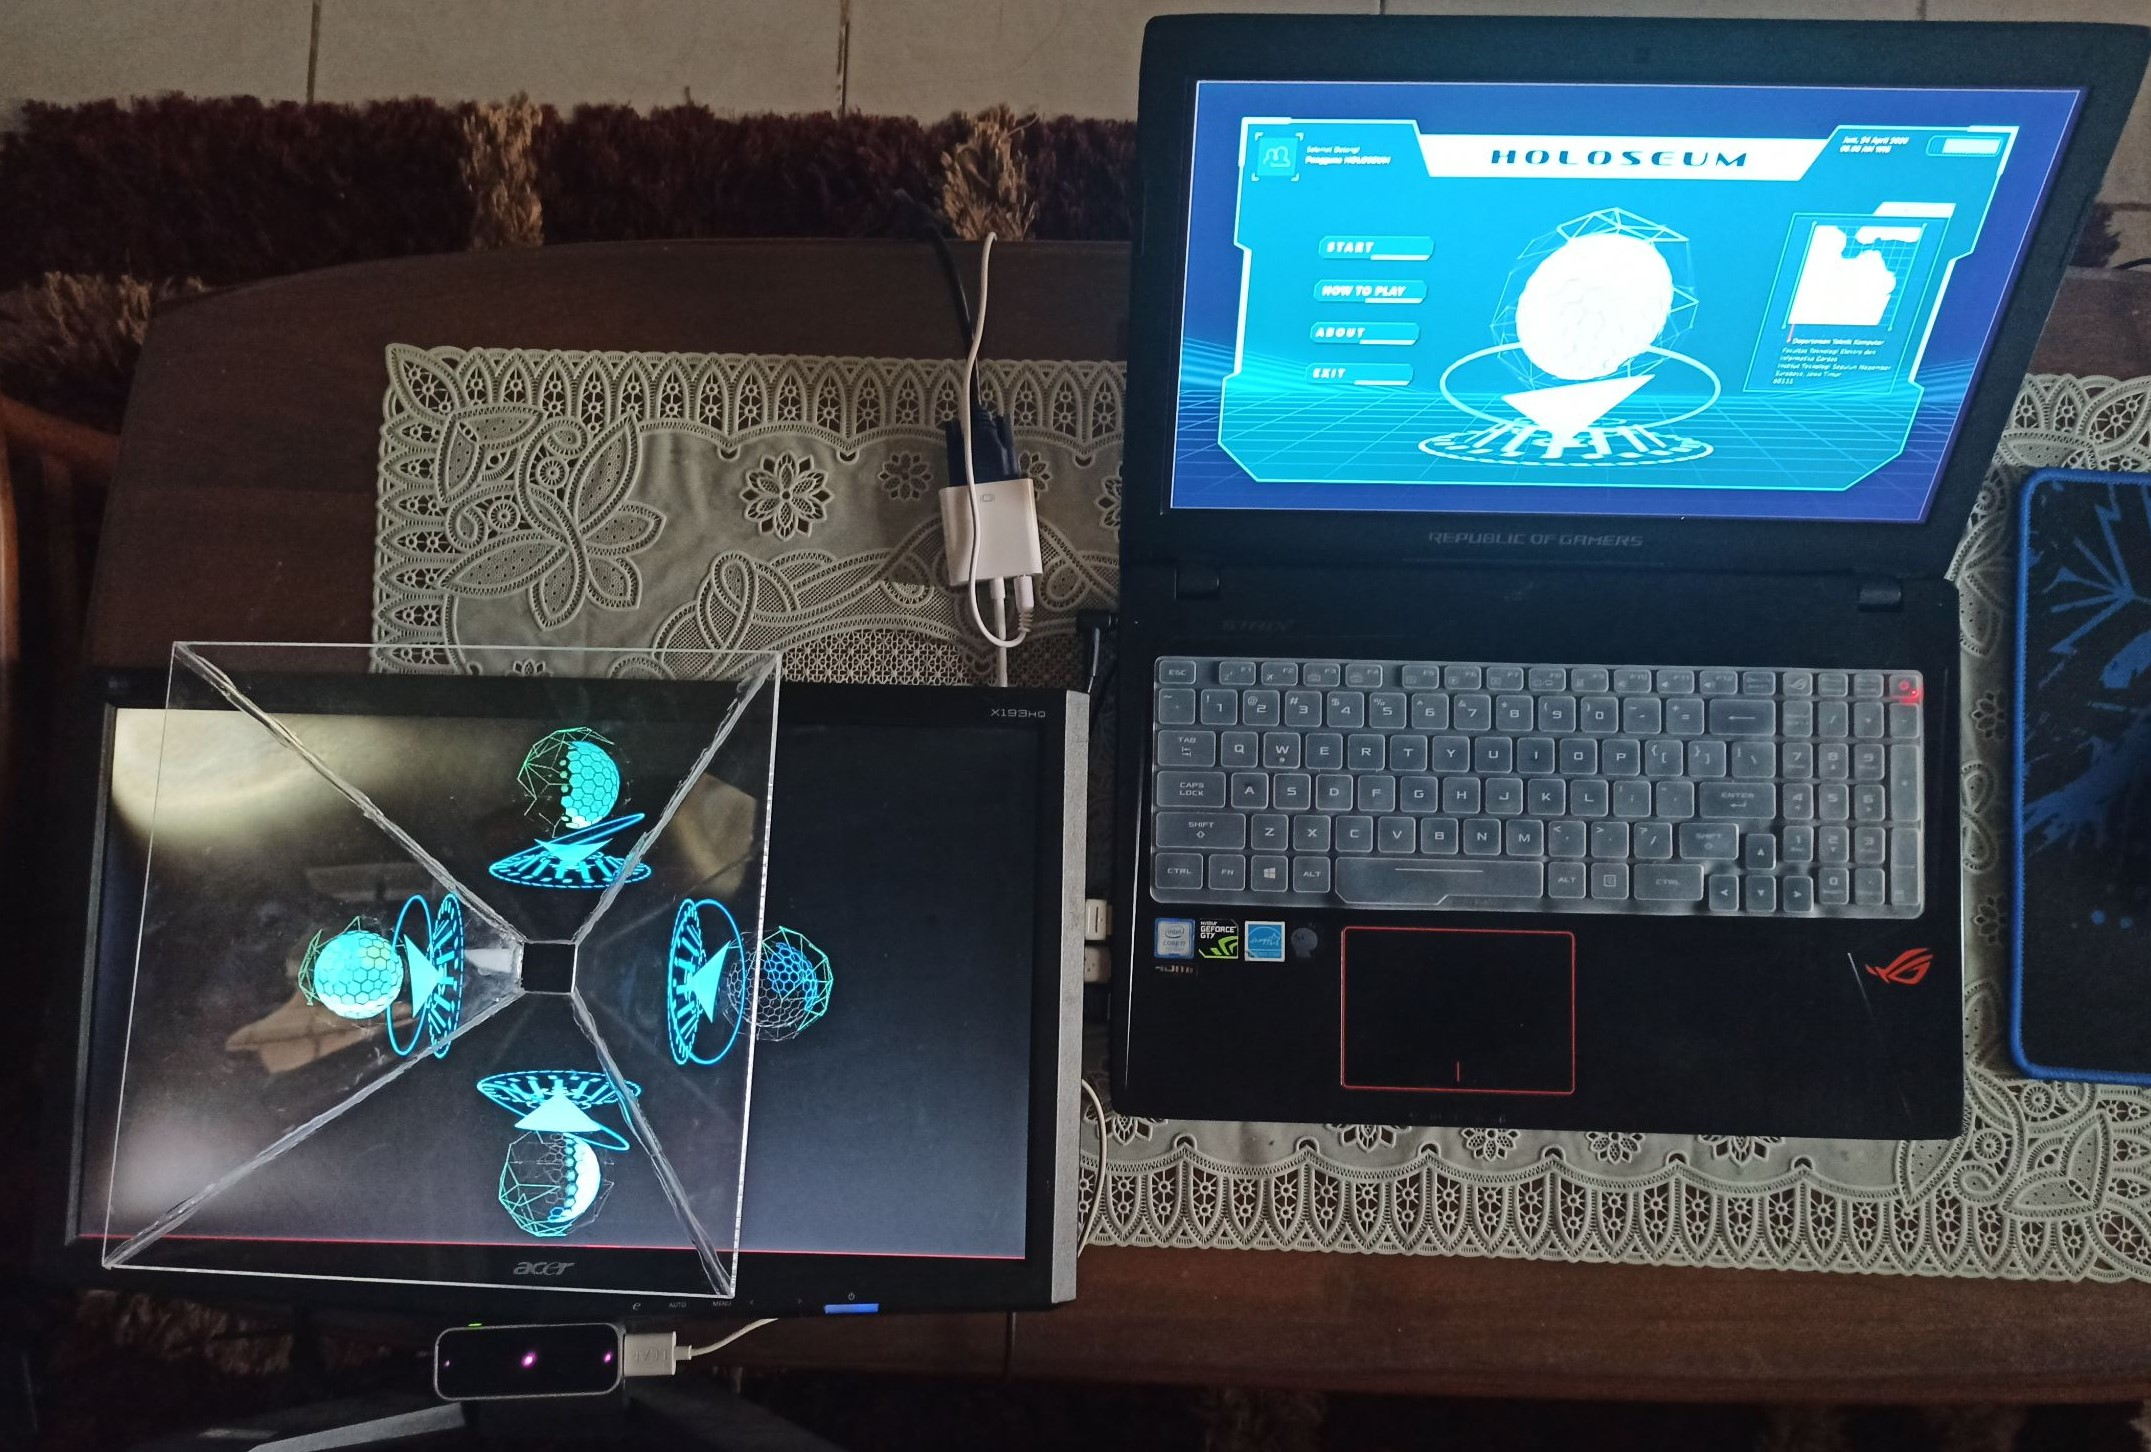
\includegraphics[width=0.33\textwidth]{img/foto_alat.jpg}}
			\caption{Setting perangkat yang dibangun.}
			\label{fig:foto_alat}
		\end{figure}
	
	\subsection{Sistem Visualisasi Hologram}
		Sistem visualisasi yang diterapkan pada penelitian ini berkaitan dengan penyajian program di \textit{display} dan komputer server. Alur dalam membangun sistem visualisasi ini ditunjukkan pada gambar \ref{fig:desain_visualisasi}.
		\vspace{-2ex}
		\begin{figure} [h]
			\centering{
\includegraphics[width=0.49\textwidth]{img/desain_visualisasi.png}}
			\caption{Alur kerja sistem visualisasi hologram.}
			\label{fig:desain_visualisasi}
		\end{figure}
		\vspace{-2ex}
		
		Penyesuaian objek 3D terjadi melalui beberapa proses. Proses pertama yaitu memodifikasi detail objek berdasarkan elemen penyusunnya, seperti menambah atau mengurangi elemen penyusun dan memindah titik tengahnya. Proses kedua bertujuan untuk mengatur objek dan membangun fitur pelengkap. Objek yang telah di-\textit{import} diposisikan pada tengah \textit{camera setting} dan diatur ukurannya melalui \textit{scale}. Kemudian mengatur nilai standard, menambahkan komponen \textit{rigidbody} dan \textit{collider} agar dapat berinteraksi dengan asset Leap Motion dan membangun fitur respons berdasarkan gesturnya. Penyesuaian terakhir dilakukan untuk memberikan efek hologram pada material objek 3D. 
		
		Objek 3D yang telah disesuaikan selanjutnya direkonstruksi menjadi \textit{hologram video} untuk menyesuaikan tampilan pada monitor dengan mengatur penempatan objek 3D tepat di setiap sisi \textit{pyramid hologram}. Untuk menampilkan 4 posisi objek pada 1 \textit{game view} seperti gambar \ref{fig:unity_12cam}, pengaturan yang diterapkan pada penelitian ini berupa sebuah objek 3D yang dikelilingi oleh 4 \textit{main camera} yang berbeda dan 7 \textit{hidden camera} untuk menampilkan \textit{background} hitam.
		\begin{figure} [h]
			\centering{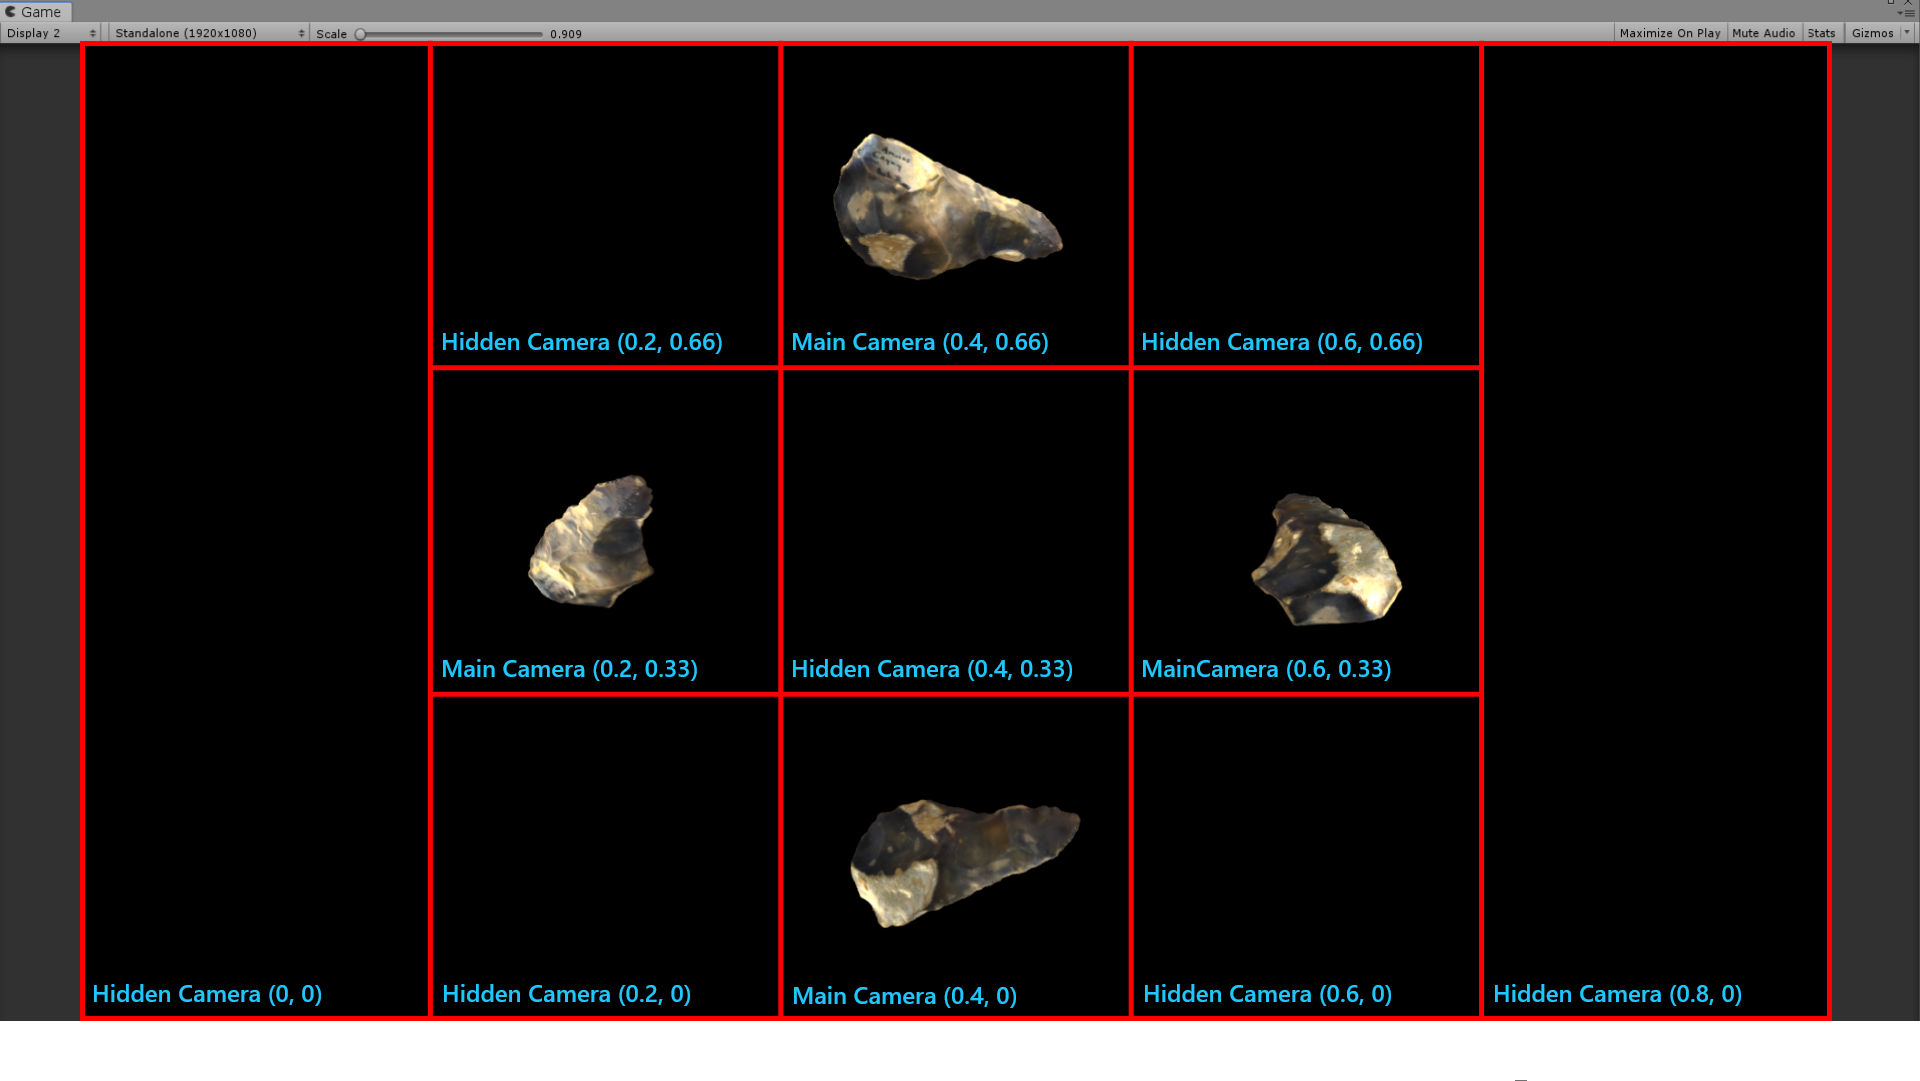
\includegraphics[width=0.4\textwidth]{img/unity_12cam.png}}
			\vspace{-1ex}
			\caption{Pengaturan \textit{viewport} untuk \textit{hologram video}.}
			\label{fig:unity_12cam}
		\end{figure}
		\vspace{-2ex}
	
		Objek yang ditampilkan pada \textit{display monitor} juga ditampilkan informasinya melalui \textit{information monitor}. Bagian pertama berupa \textit{Main Menu} atau Menu Utama merupakan tampilan awal saat aplikasi tersebut dijalankan. Terdiri dari tombol \textit{Start} untuk menuju \textit{Main Scene}, \textit{How to Play} untuk menunjukkan cara permainan, \textit{About} untuk menunjukkan informasi mengenai produk dan \textit{developer}, dan \textit{Exit} untuk keluar dari aplikasi yang ditunjukkan pada gambar \ref{fig:mainmenu}.
		
		Sedangkan \textit{Main Scene} adalah \textit{scene} utama atau \textit{gameplay} yang menampilkan objek hologram beserta informasi dan foto aslinya. Terdapat pula tombol \textit{Next} dan \textit{Previous} berfungsi untuk mengganti objek yang ditampilkan, baik pada \textit{display monitor} maupun \textit{information monitor}. Icon "animasi" menunjukkan apakah objek hologram tersebut memiliki animasi yang dapat diputar sesuai dengan gestur yang bersesuaian. 
		\begin{figure} [h]
			\begin{subfigure}[t]{0.23\textwidth}
				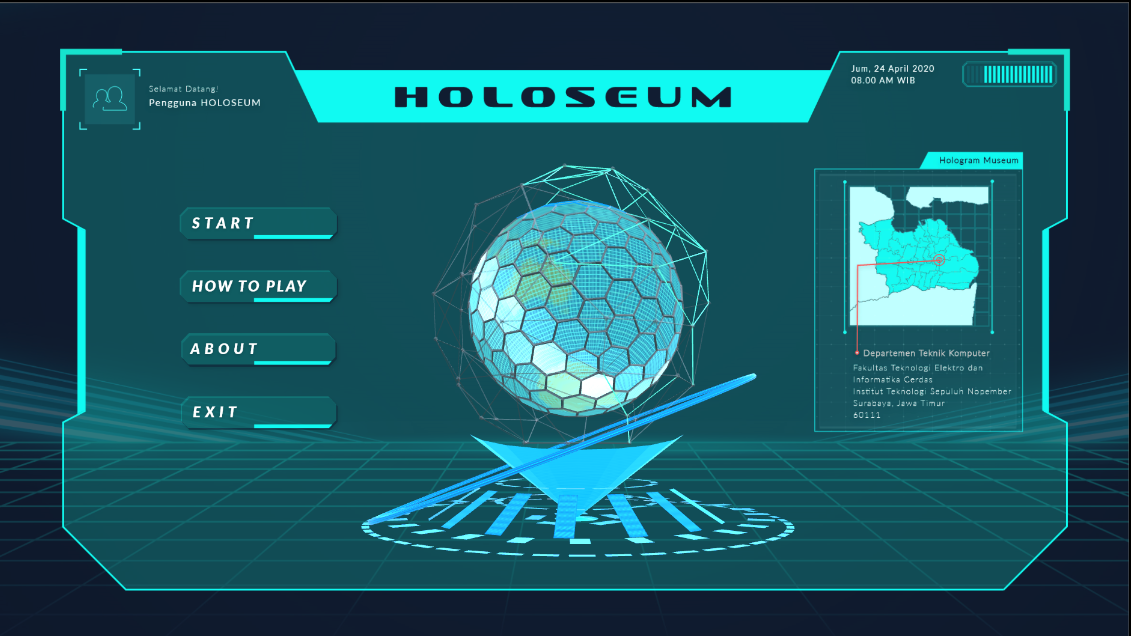
\includegraphics[width=\textwidth]{img/mainmenu.png}
				\caption{\textit{Main Menu}.\label{fig:mainmenu}}
			\end{subfigure}
			\hspace{0.1em}
			\begin{subfigure}[t]{0.23\textwidth}
				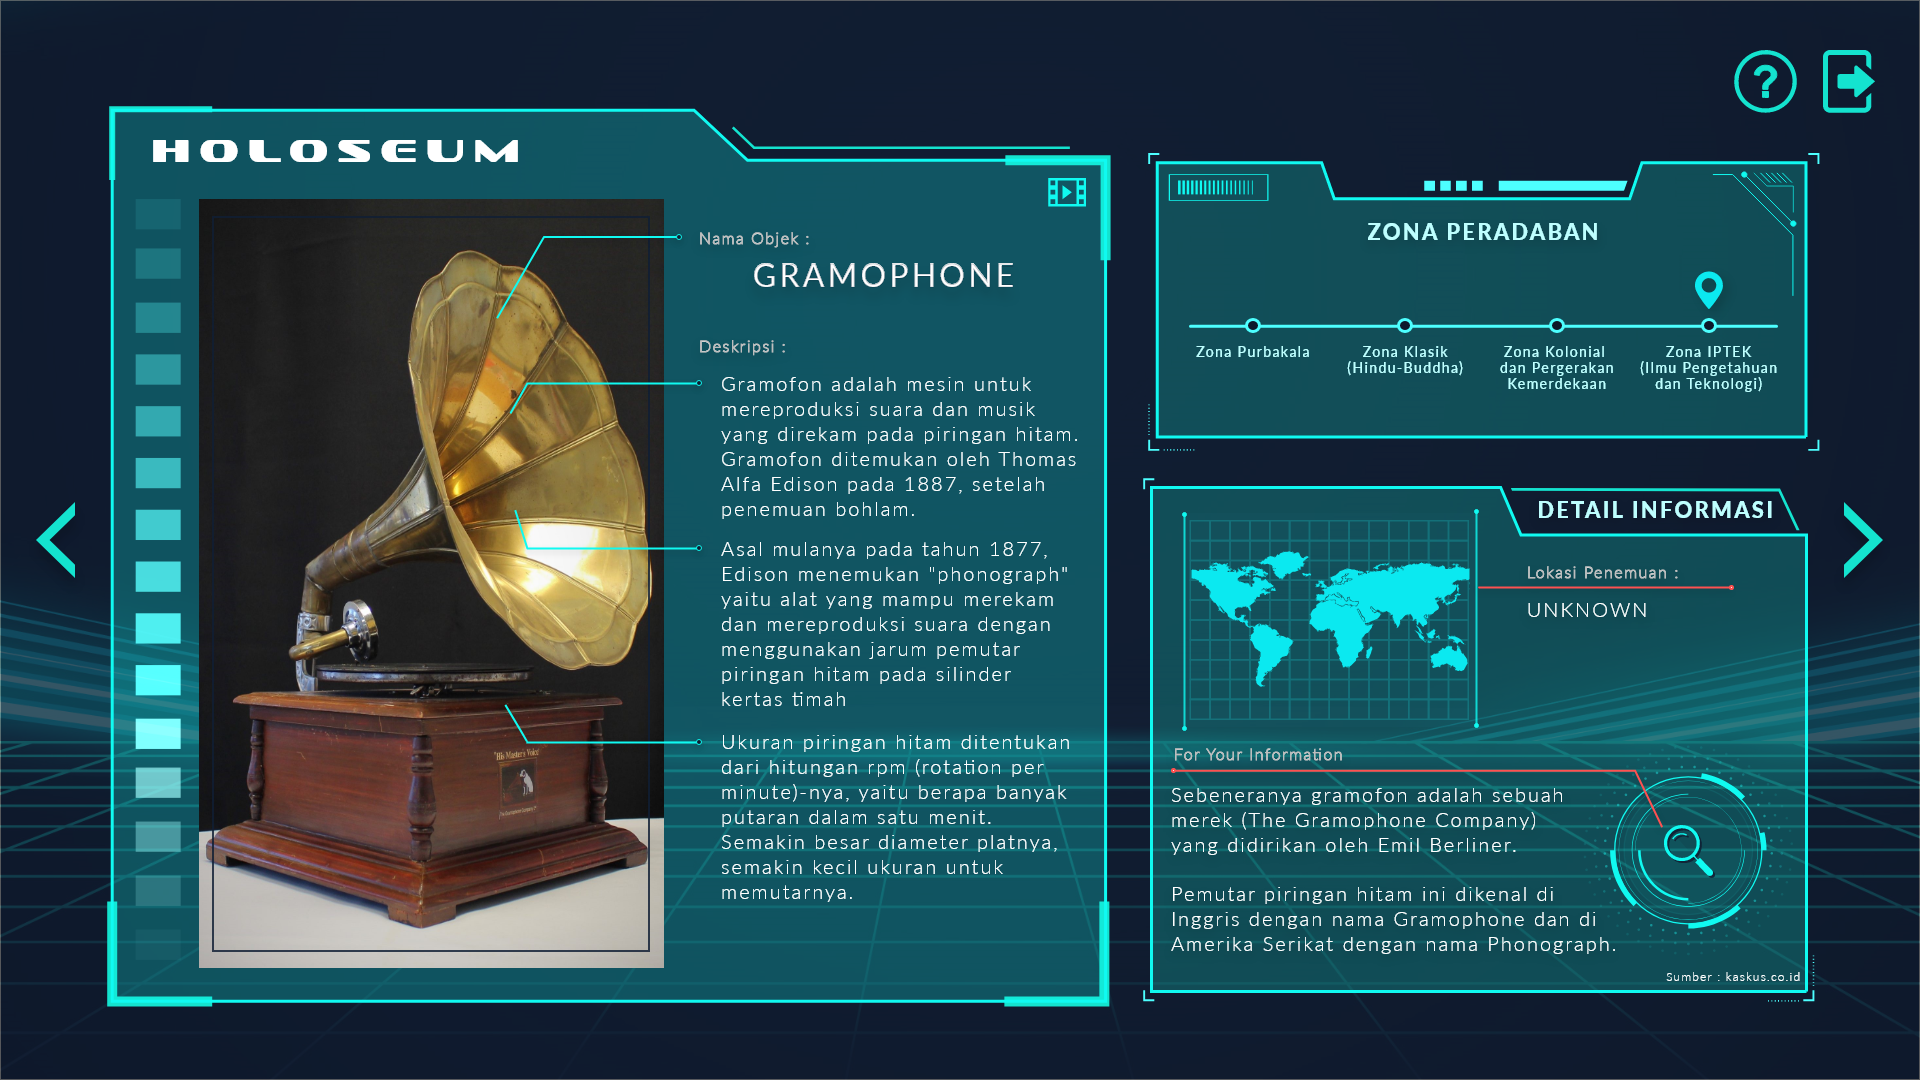
\includegraphics[width=\textwidth]{img/mainscene.png}
				\caption{\textit{Main Scene}.\label{fig:mainscene}}
			\end{subfigure}
			\vspace{-1ex}
			\caption{Tampilan aplikasi.}
		\end{figure}
		\vspace{-2ex}
	
	\subsection{Sistem Interaksi Pengindera Tangan}
		Sistem interaksi yang diterapkan pada penelitian ini berkaitan dengan proses deteksi pola tangan dan aktivasi fitur-respons yang dibangun. Alur kerja dari sistem interaksi yang diterapkan ditunjukkan pada gambar \ref{fig:desain_interaksi}.
		\vspace{-2ex}
		\begin{figure}[h]
			\centering{
\includegraphics[width=0.49\textwidth]{img/desain_interaksi.png}}
			\caption{Alur kerja sistem interaksi pengindera tangan.}
			\label{fig:desain_interaksi}
		\end{figure}
		\vspace{-2ex}
		
		Pola tangan dapat diketahui apabila kondisi setiap \textit{hand object elements} yang membangunnya dalam keadaan aktif. Setiap \textit{detector} hanya dapat mendeteksi satu jenis elemen, sehingga jika ingin mendeteksi beberapa elemen sekaligus membutuhkan \textit{detector logic gate} selayaknya \textit{logic gate} AND dan OR maupun negasinya. Gestur tangan yang dibangun pada penelitian ini ditunjukkan melalui gambar \ref{fig:gestur_interaksi}.
		
		\subsubsection{Algoritma Eksplorasi Objek}
			Eksplorasi objek yang dapat dilakukan oleh pengguna adalah dengan menggenggam objek untuk melihat objek hologram dari segala sisi menggunakan gestur \ref{fig:gs1a} dan \ref{fig:gs1b}. Objek hologram yang dieksplorasi akan merespon gestur secara berputar pada porosnya maupun bergerak pada area yang telah ditentukan berdasarkan perubahan posisi dan rotasi pada tangan yang didapatkan dari perpindahan (selisih) antar \textit{frame}. Persamaan \ref{eqn:position_target} digunakan untuk menghitung nilai posisi sedangkan persamaan \ref{eqn:rotation_target} untuk mendapatkan nilai rotasi.
			
			\vspace{-2ex}			
			\begin{equation}
			\begin{alignedat}{2}
			& \overrightarrow{V_{C}} &&= \overrightarrow{V_{B}} - \overrightarrow{V_{A}}\\
			%& 		&&= (V_{B}.x - V_{A}.x, V_{B}.y - V_{A}.y, V_{B}.z - V_{A}.z)\\
			& 		&&= (\overrightarrow{V_{B}}.x - \overrightarrow{V_{A}}.x, \overrightarrow{V_{B}}.y - \overrightarrow{V_{A}}.y, \overrightarrow{V_{B}}.z - \overrightarrow{V_{A}}.z)\\
			%& 		&&= ({V_{B}}_{x} \uvec{i} - {V_{A}}_{x} \uvec{i}, {V_{B}}_{y} \uvec{j} - {V_{A}}_{y} \uvec{j}, {V_{B}}_{z} \uvec{k} - {V_{A}}_{z} \uvec{k})
			%& 		&&= (x_{\overrightarrow{V_{B}}} - x_{\overrightarrow{V_{A}}}, y_{\overrightarrow{V_{B}}} - y_{\overrightarrow{V_{A}}}, z_{\overrightarrow{V_{B}}} - z_{\overrightarrow{V_{A}}})\\	
			\end{alignedat}
			\label{eqn:position_target}
			\end{equation}
			
			\begin{equation}
			\begin{alignedat}{3}
			\overrightarrow{Q_{A}} \cdot & \overrightarrow{Q_{C}} &&= \overrightarrow{Q_{B}}\\ 
			\overrightarrow{Q_{A}} \cdot \overrightarrow{\inv{Q_{A}}} \cdot& \overrightarrow{Q_{C}} &&= \overrightarrow{\inv{Q_{A}}} \cdot \overrightarrow{Q_{B}}\\
			\overrightarrow{I} \cdot & \overrightarrow{Q_{C}} &&= \overrightarrow{\inv{Q_{A}}} \cdot \overrightarrow{Q_{B}}\\
			&\overrightarrow{Q_{C}} &&= \overrightarrow{\inv{Q_{A}}} \cdot \overrightarrow{Q_{B}}\\
			\end{alignedat}
			\label{eqn:rotation_target}
			\end{equation}
		
		\subsubsection{Algoritma \textit{Zoom Object}}
			\textit{Zoom Object} adalah fitur yang dapat memperbesar dan memperkecil objek hologram hingga mencapai nilai maksimal yang telah ditentukan melalui gestur \ref{fig:gs2}. Fitur ini membantu pengguna untuk melihat detail objek dalam ukuran yang berbeda berdasarkan jarak antar kedua tangan yang diwakili jari telunjuk (\textit{index finger}). Jarak antara kedua tangan digunakan untuk menghitung rasio skala perbesaran sesuai persamaan \ref{eqn:zoom_scale}.
			\begin{equation}
			ScaleValue = \frac{distanceValue}{maxDistance} \cdot maxScale
			\label{eqn:zoom_scale}
			\end{equation}
			
		\subsubsection{Algoritma Aktivasi Animasi Objek}
			Fitur ini memungkinkan pengguna untuk mengaktivasi dan melihat pergerakan animasi dari objek yang bersesuain menggunakan salah satu gestur \ref{fig:gs3a}, \ref{fig:gs3b}, ataupun \ref{fig:gs3c}. Pada penelitian ini, objek yang dapat dilihat animasinya adalah \textit{primeval axe} dan \textit{gramophone} yang ditunjukkan melalui ikon "animated" pada \textit{information monitor}.
		
		\subsubsection{Algoritma \textit{Reset to Default}}
			\textit{Reset to default} adalah fitur yang mengembalikan objek pada posisi, rotasi, dan ukuran semula sesuai dengan \textit{defaultnya} dengan gestur \ref{fig:gs4}. Fitur ini memungkinkan pengguna untuk melihat objek secara keseluruhan secara otomatis tanpa harus menyesuaikannya satu persatu (tanpa memindah, memutar, maupun memperkecil secara manual).
		
		\subsubsection{Algoritma Pergantian Objek}
			Pengguna dapat memilih objek sebelum maupun objek setelah dari objek yang ditampilkan saat ini. Objek hologram dan informasi yang disampaikan dapat diubah melalui gestur \ref{fig:gs5a} dan \ref{fig:gs5b} tanpa memilih tombol pada  \textit{information monitor}.
			
		\subsubsection{Algoritma Menampilkan Menu \textit{Help}}
			Saat berada dalam \textit{Main Scene}, pengguna dapat menampilkan menu \textit{Help} untuk membuka cara penggunaan perangkat berupa melihat variasi gestur yang dimiliki dan keterangan \textit{layout} informasi objek pada \textit{information monitor}. Pengguna dapat mengakses fitur ini melalui gestur \ref{fig:gs6} tanpa memilih tombol pada  \textit{information monitor}.
			
		\subsubsection{Algoritma Menampilkan \textit{Main Menu}}
			Fitur ini serupa dengan Algoritma Menampilkan Menu \textit{Help}, hanya saja menu yang ditampilkan adalah \textit{Main Menu} atau dapat dikenal juga untuk keluar dari \textit{Main Scene}. Gestur pada algoritma ini serupa dengan gestur \textit{high five} pada Algoritma \textit{Reset to Default} (gambar \ref{fig:gs4}), yang membedakan adalah jarak \textit{thumb finger} dan \textit{index finger} menentukan aktivasi respons (gambar \ref{fig:gs7}). Jarak antar \textit{thumb finger} dan \textit{index finger} pada kedua tangan dengan persamaan \ref{eqn:position_target}.
			
		\subsubsection{Algoritma Membatalkan atau Menyetujui Pilihan}
			Ketika Main Scene dijalankan, pengguna dapat menampilkan menu \textit{Help} dan \textit{Main Menu} yang terdapat beberapa tombol. Pengguna juga dapat mengakses tombol tersebut menggunakan gestur yang bersesuaian. Tombol untuk membatalkan pilihan (\textit{back} dan \textit{cancel}) dapat diakses menggunakan gestur \ref{fig:gs8a} dan \ref{fig:gs8b}. Sedangkan tombol untuk menyetujui pilihan (OK) dapat diakses menggunakan gestur \ref{fig:gs8c} dan \ref{fig:gs8d}.
				
		\begin{figure} [h]
			\begin{center}
			\begin{subfigure}[t]{0.11\textwidth}
				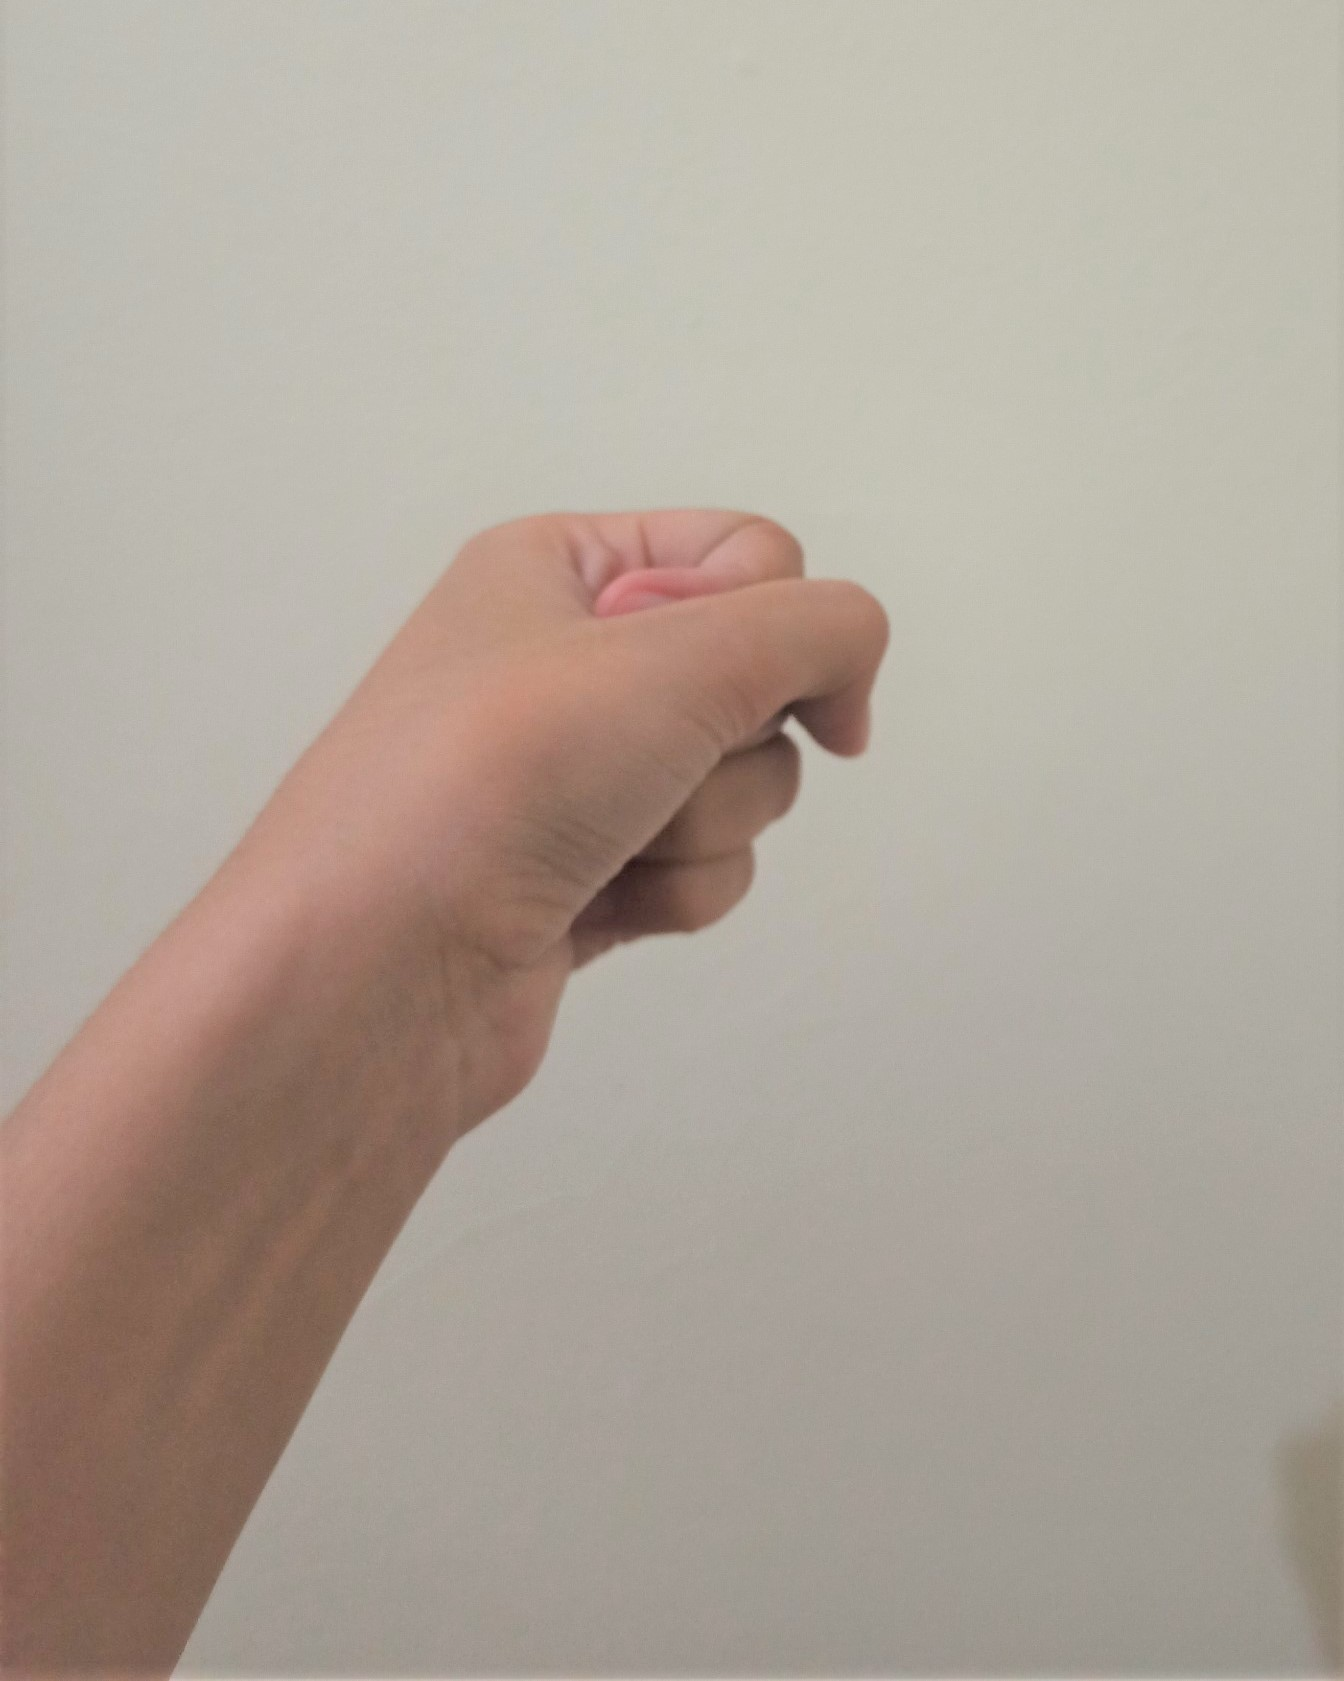
\includegraphics[width=\textwidth]{img/pola1a.jpg}
				\caption{\label{fig:gs1a}}
			\end{subfigure}
			\hspace{0.1em}
			\begin{subfigure}[t]{0.11\textwidth}
				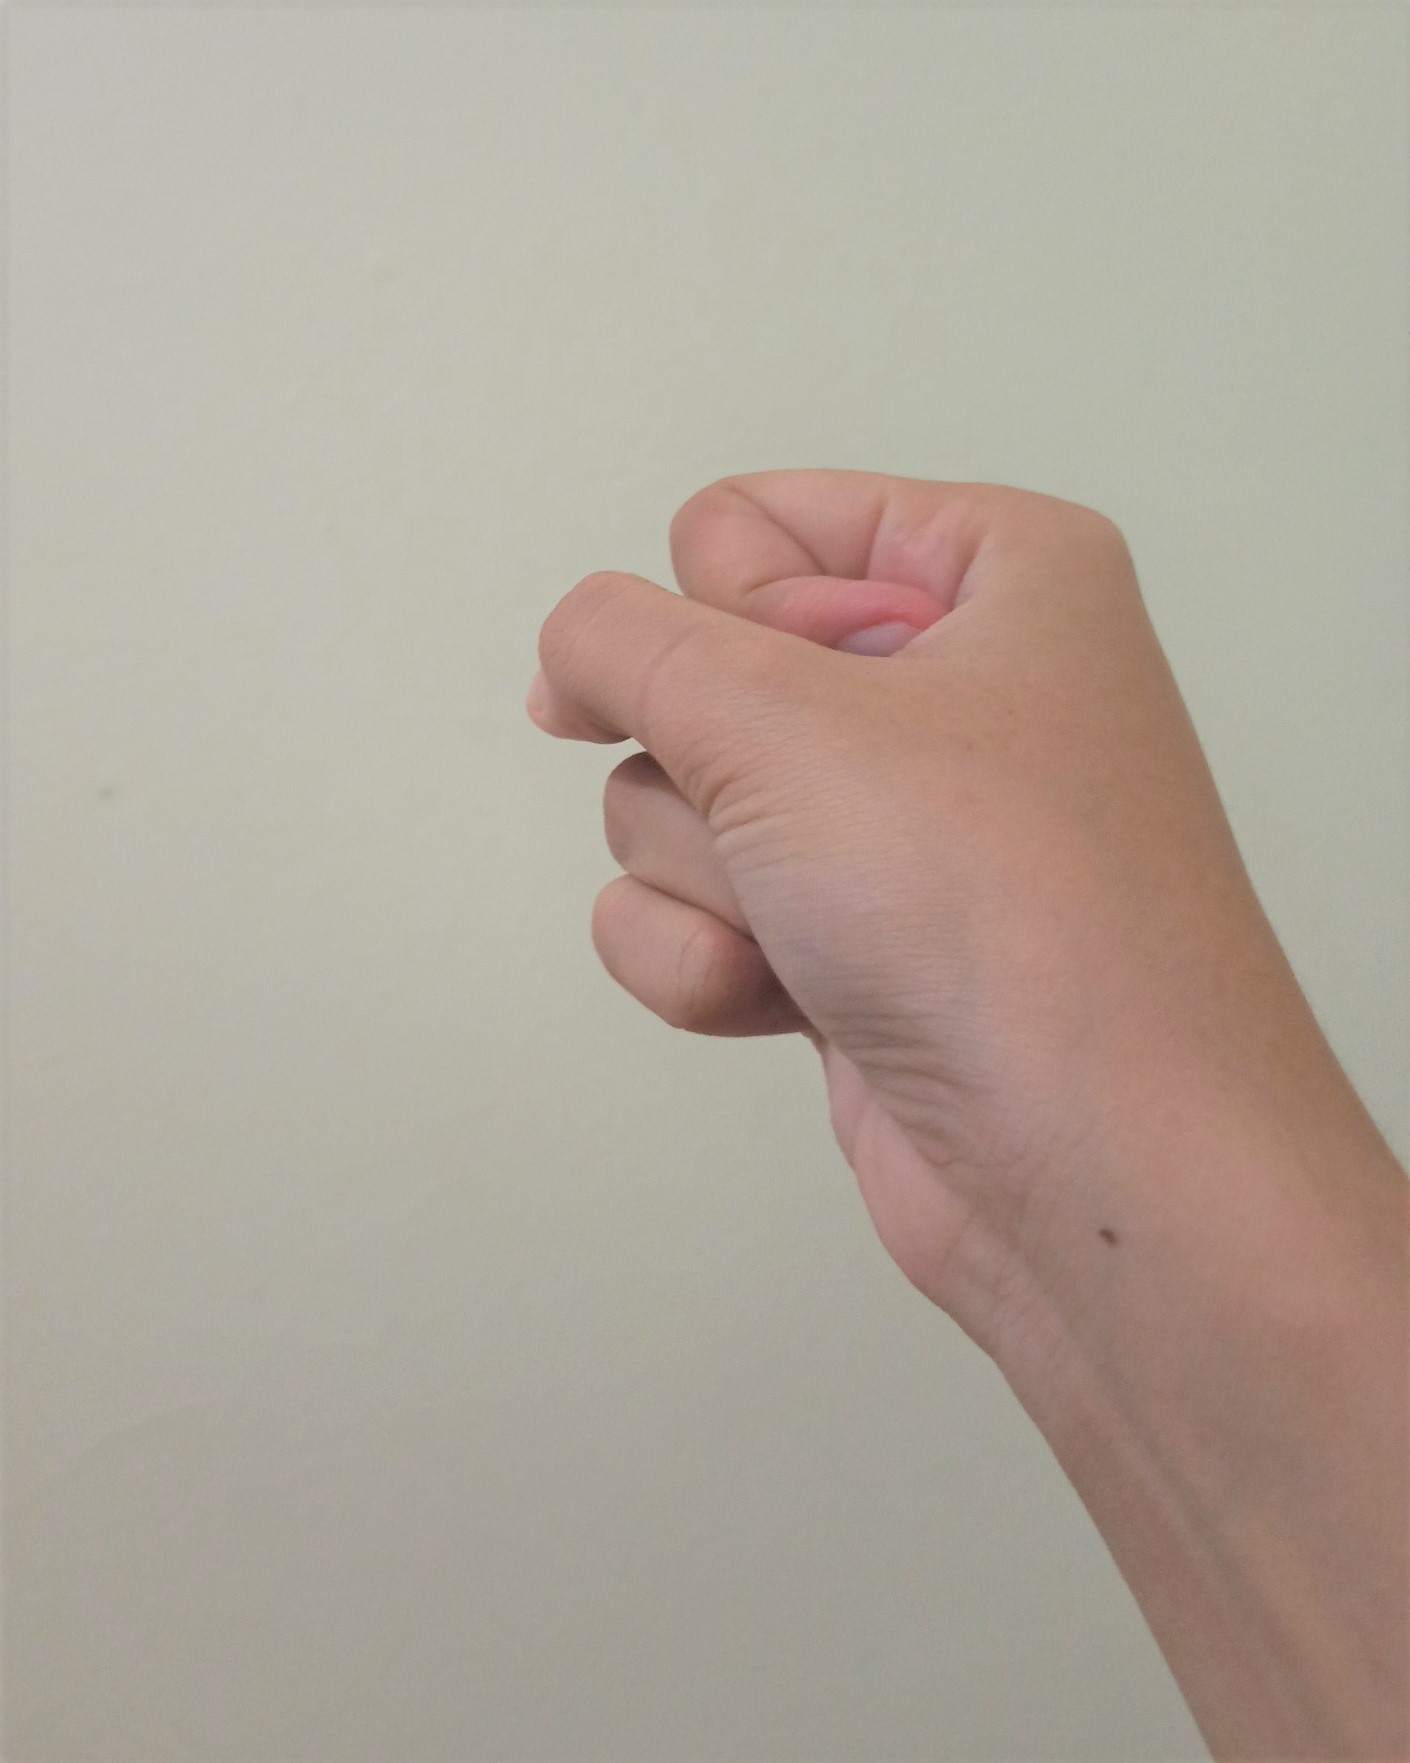
\includegraphics[width=\textwidth]{img/pola1b.jpg}
				\caption{\label{fig:gs1b}}
			\end{subfigure}
			\hspace{0.1em}
			\begin{subfigure}[t]{0.11\textwidth}
				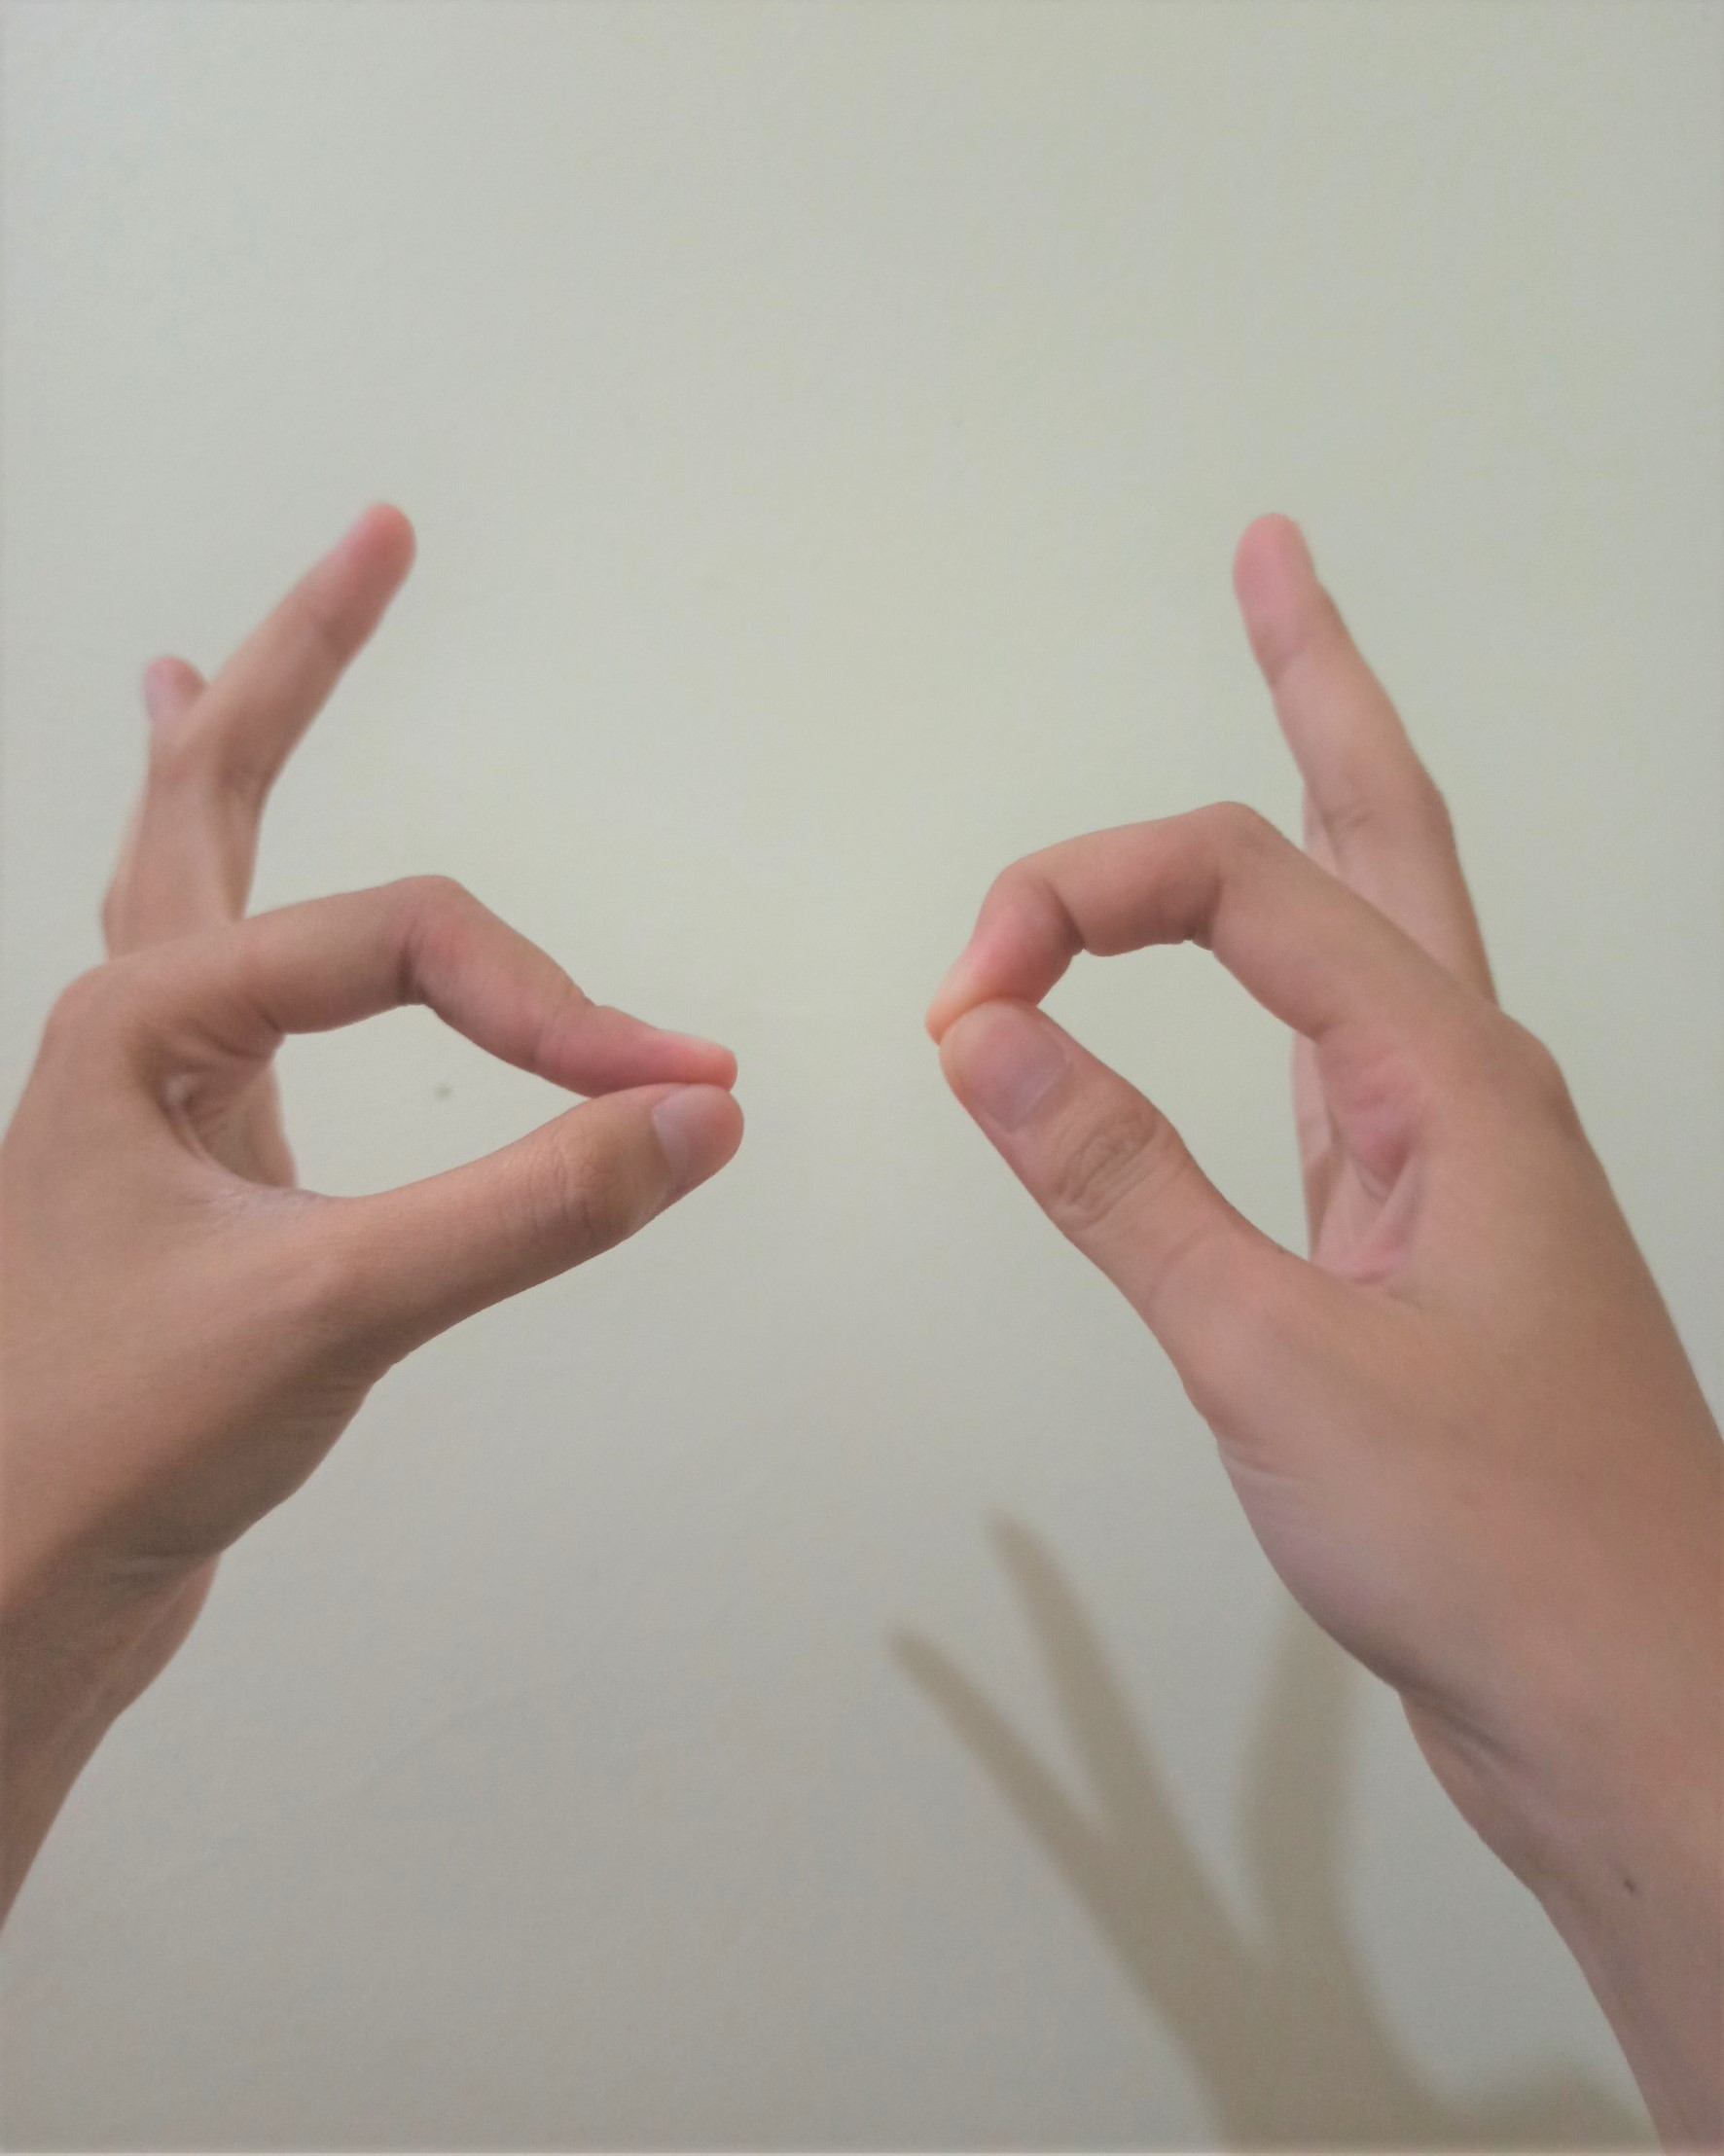
\includegraphics[width=\textwidth]{img/pola2.jpg}
				\caption{\label{fig:gs2}}
			\end{subfigure}
			\hspace{0.1em}
			\begin{subfigure}[t]{0.11\textwidth}
				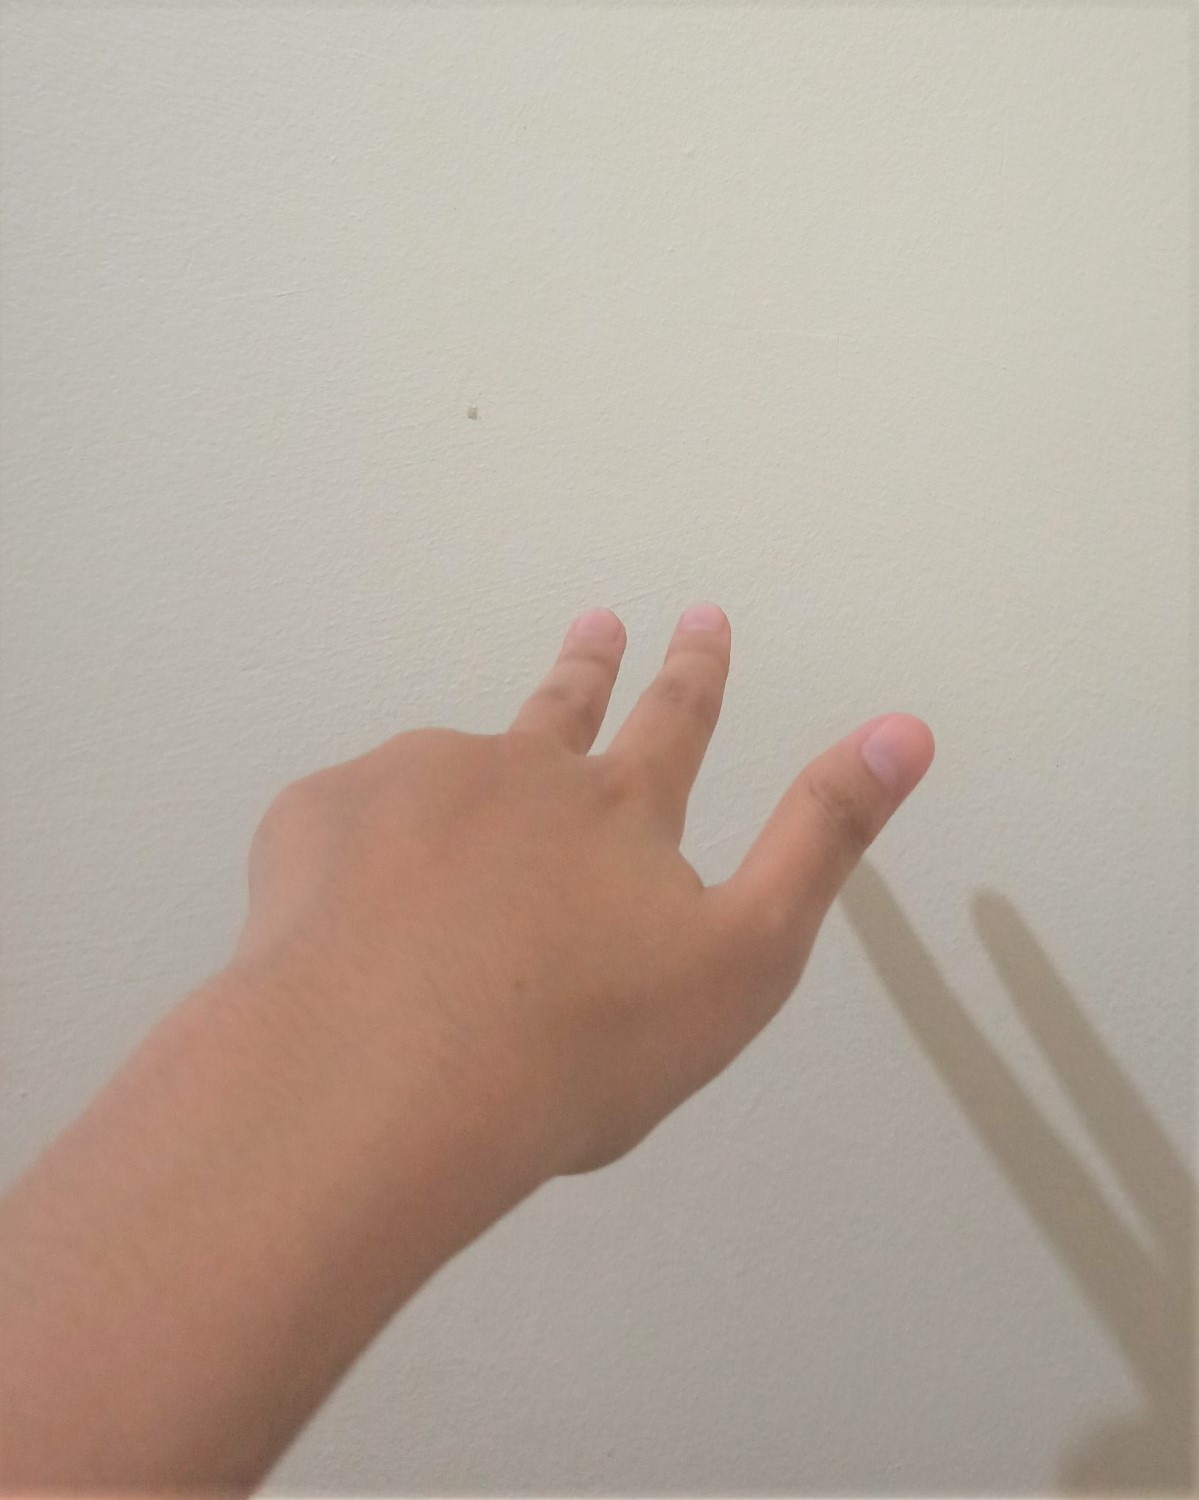
\includegraphics[width=\textwidth]{img/pola3a.jpg}
				\caption{\label{fig:gs3a}}
			\end{subfigure}
			\hspace{0.1em}
			\begin{subfigure}[t]{0.11\textwidth}
				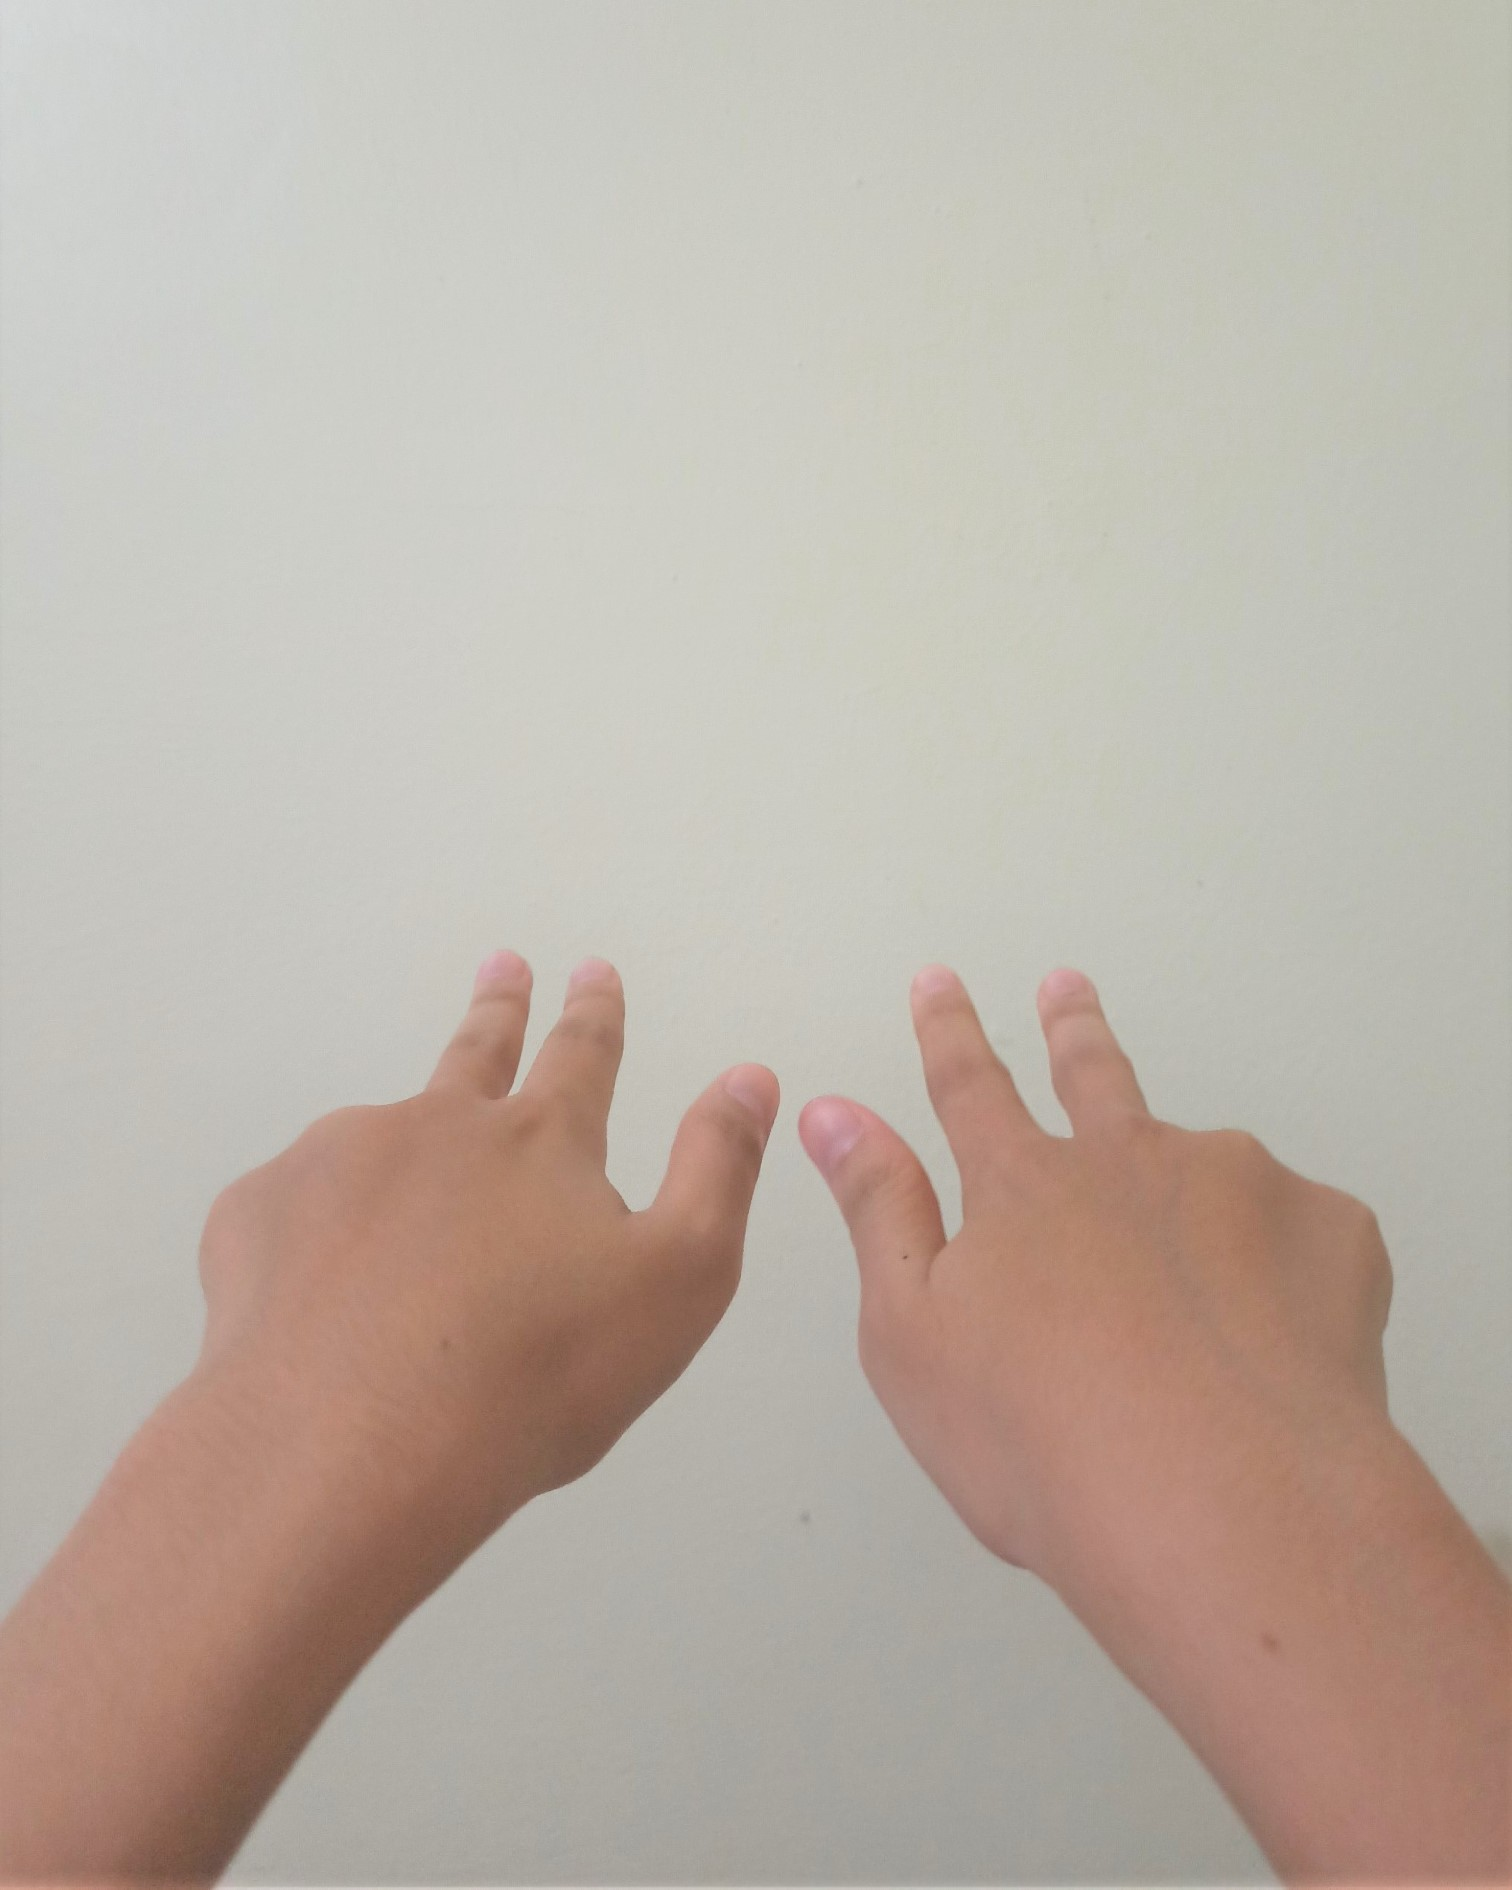
\includegraphics[width=\textwidth]{img/pola3b.jpg}
				\caption{\label{fig:gs3b}}
			\end{subfigure}
			\hspace{0.1em}
			\begin{subfigure}[t]{0.11\textwidth}
				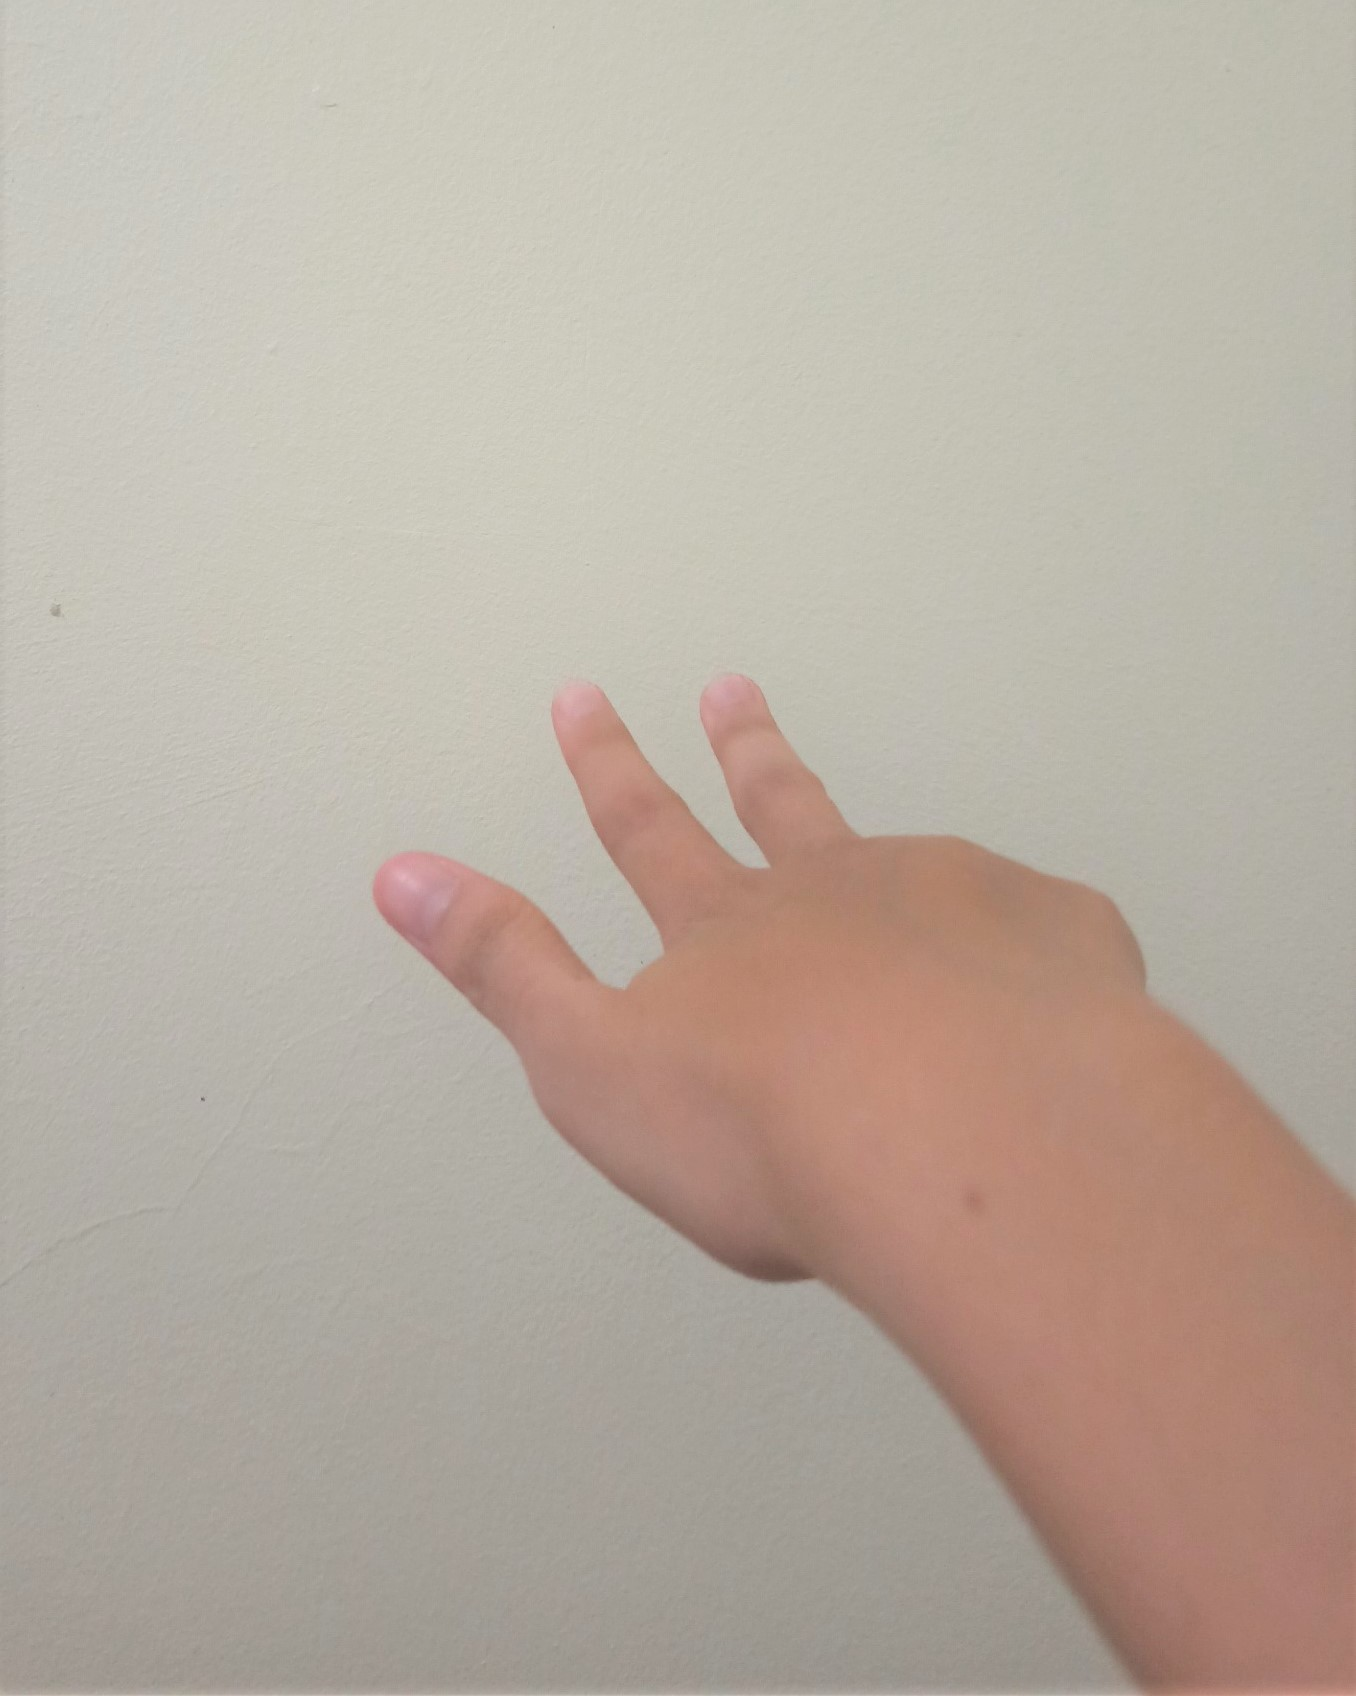
\includegraphics[width=\textwidth]{img/pola3c.jpg}
				\caption{\label{fig:gs3c}}
			\end{subfigure}
			\hspace{0.1em}
			\begin{subfigure}[t]{0.11\textwidth}
				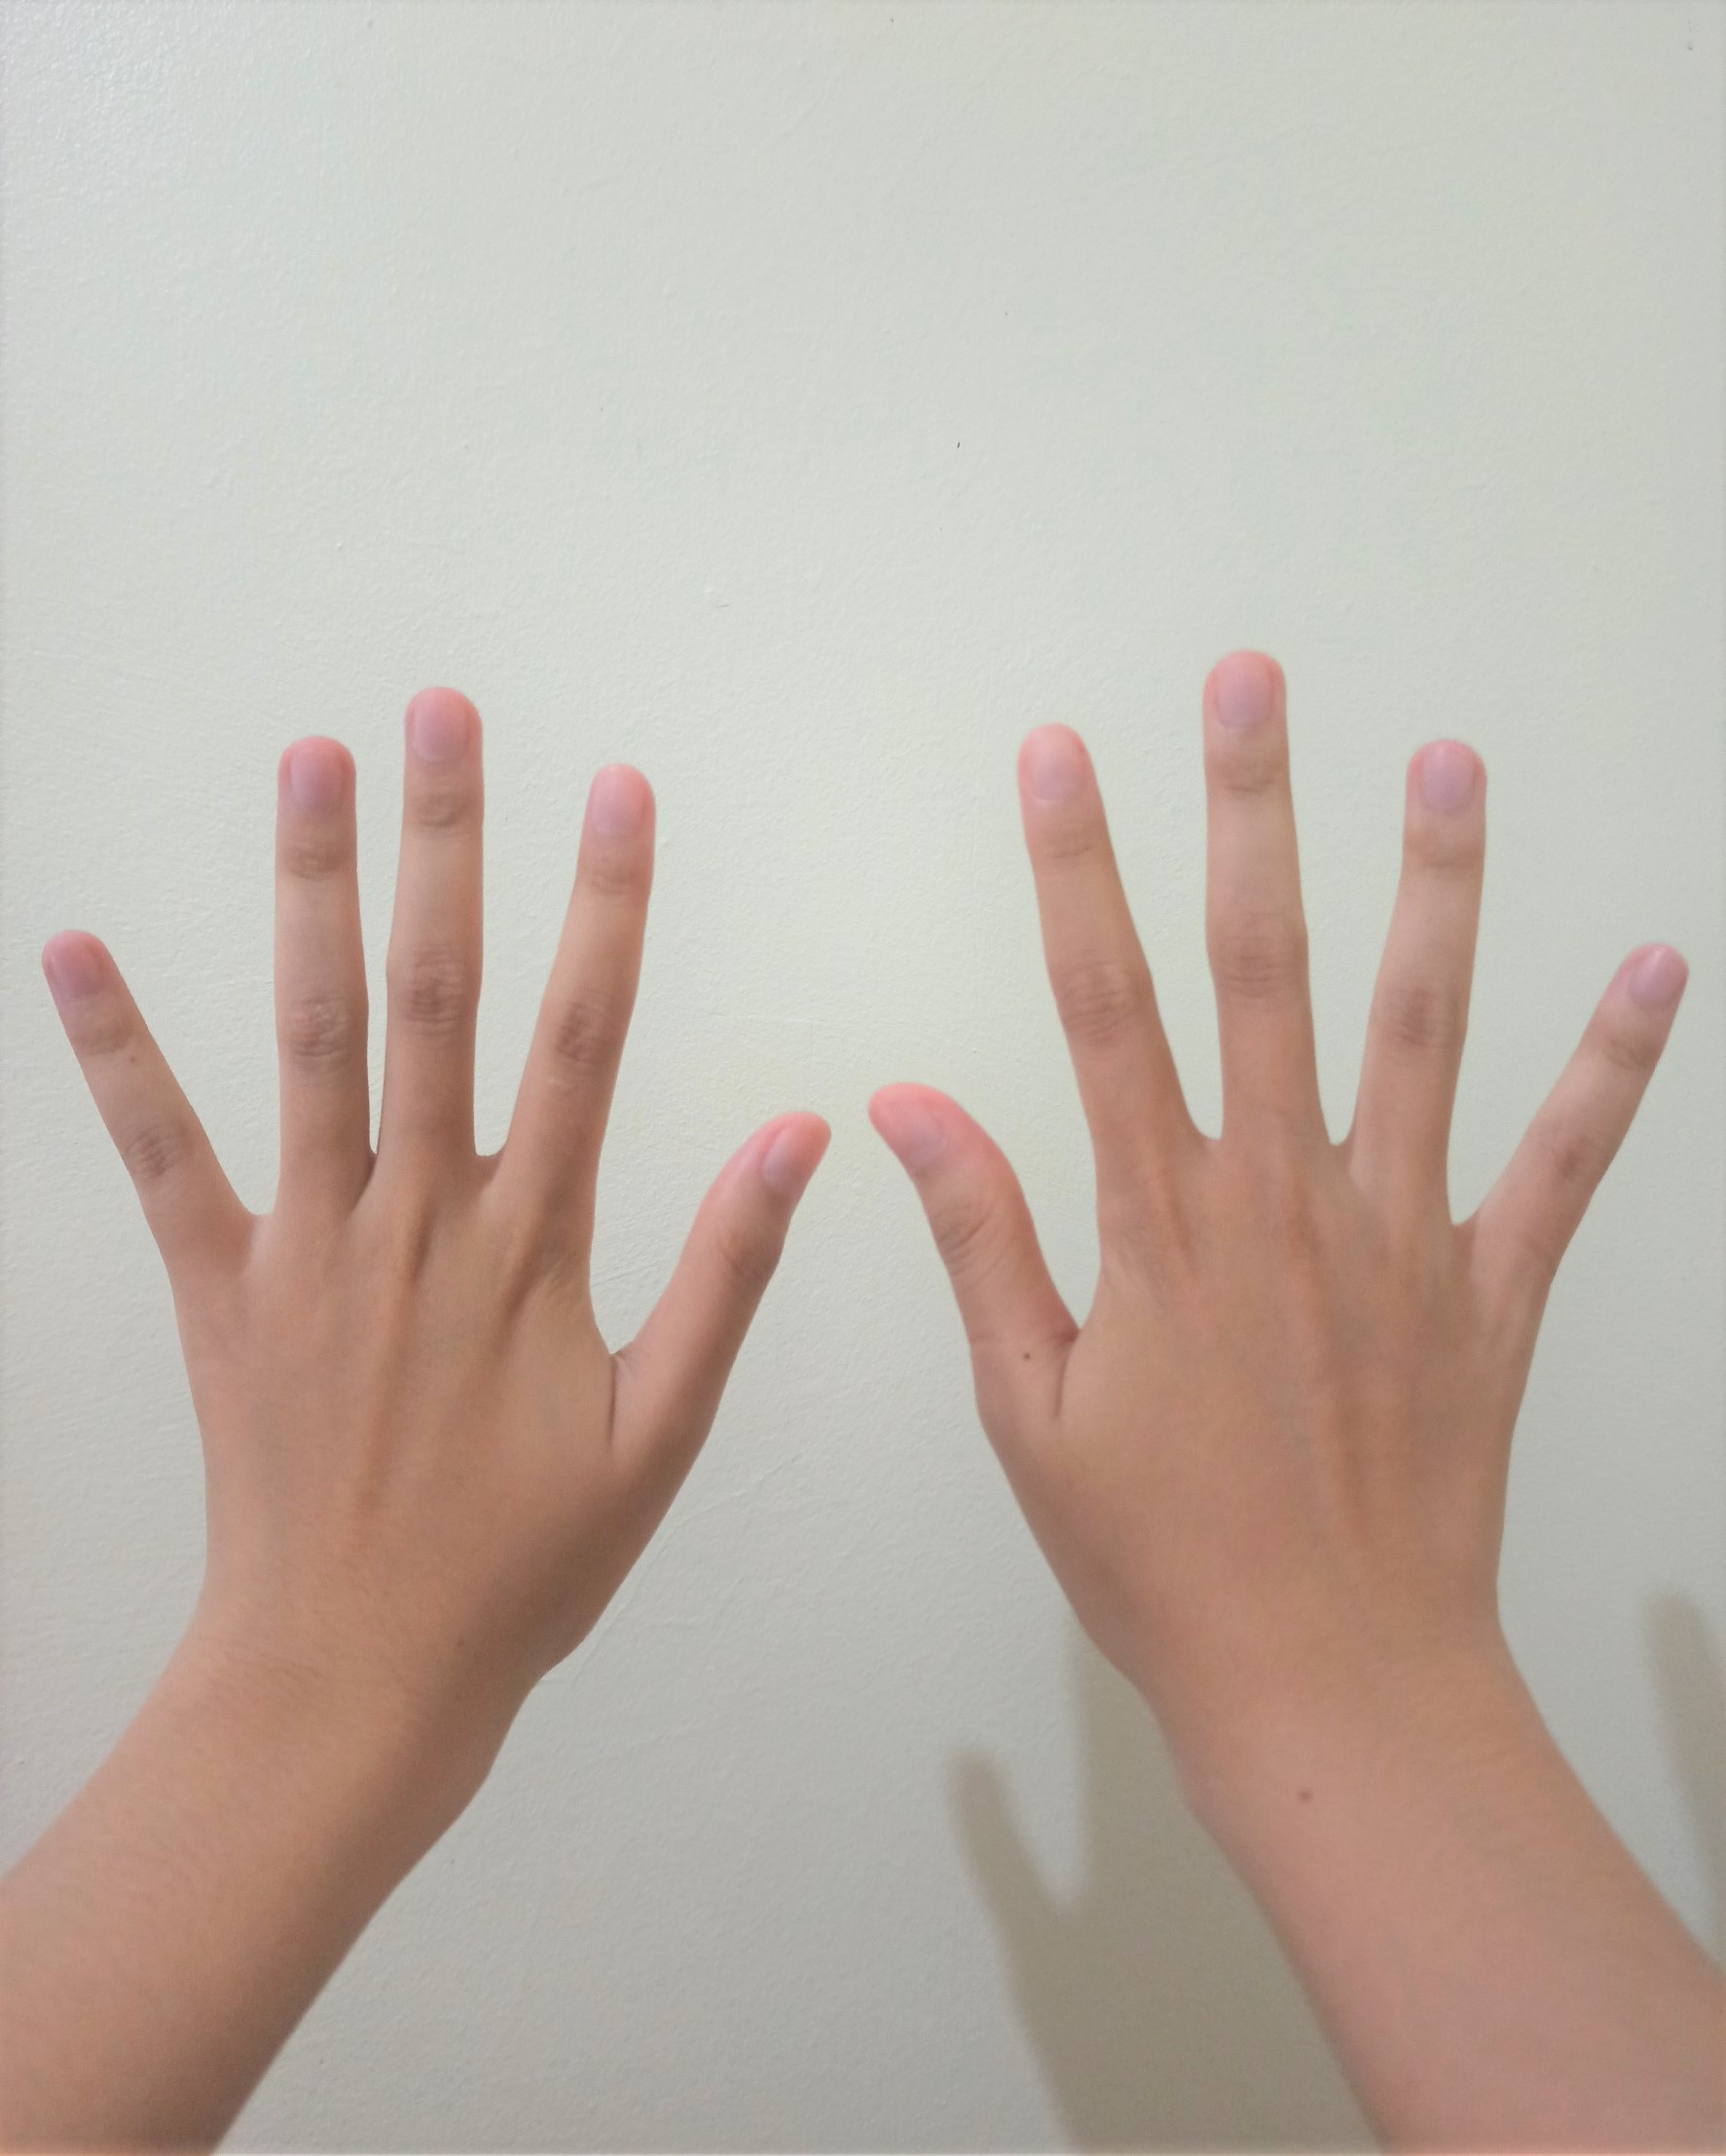
\includegraphics[width=\textwidth]{img/pola4.jpg}
				\caption{\label{fig:gs4}}
			\end{subfigure}
			\hspace{0.1em}
			\begin{subfigure}[t]{0.11\textwidth}
				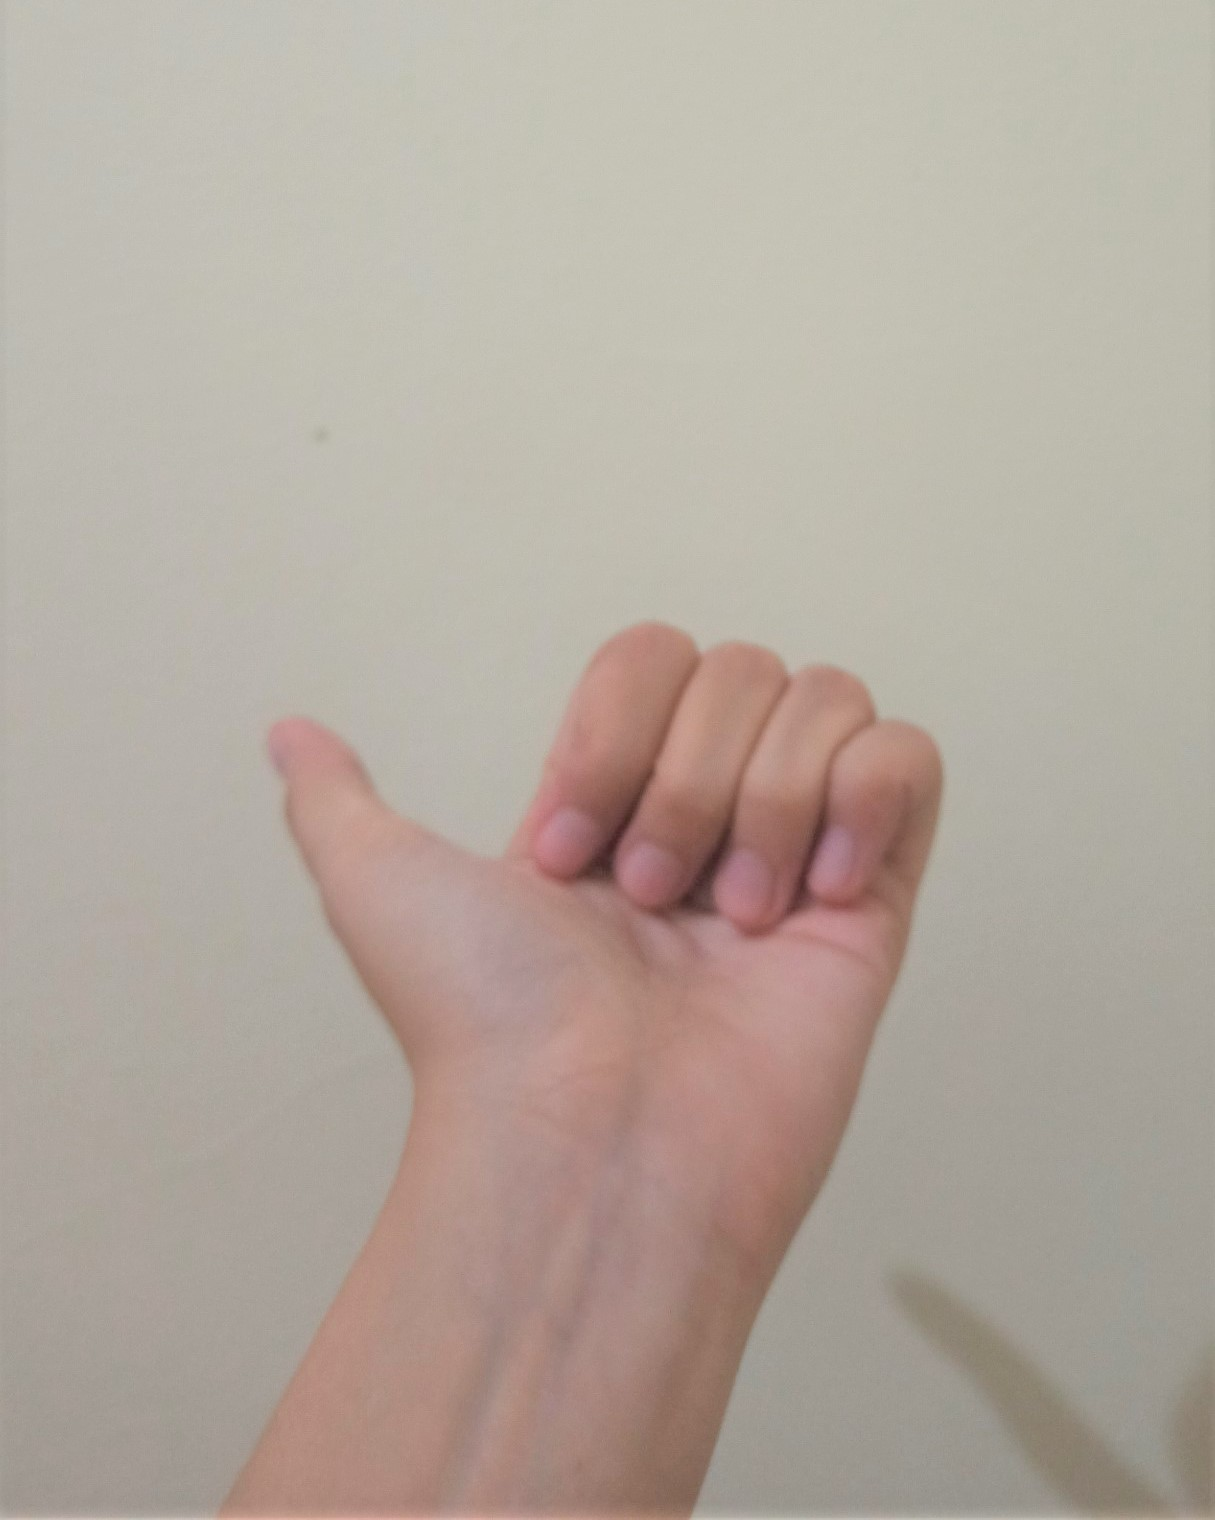
\includegraphics[width=\textwidth]{img/pola5a.jpg}
				\caption{\label{fig:gs5a}}
			\end{subfigure}
			\hspace{0.1em}
			\begin{subfigure}[t]{0.11\textwidth}
				\centering
				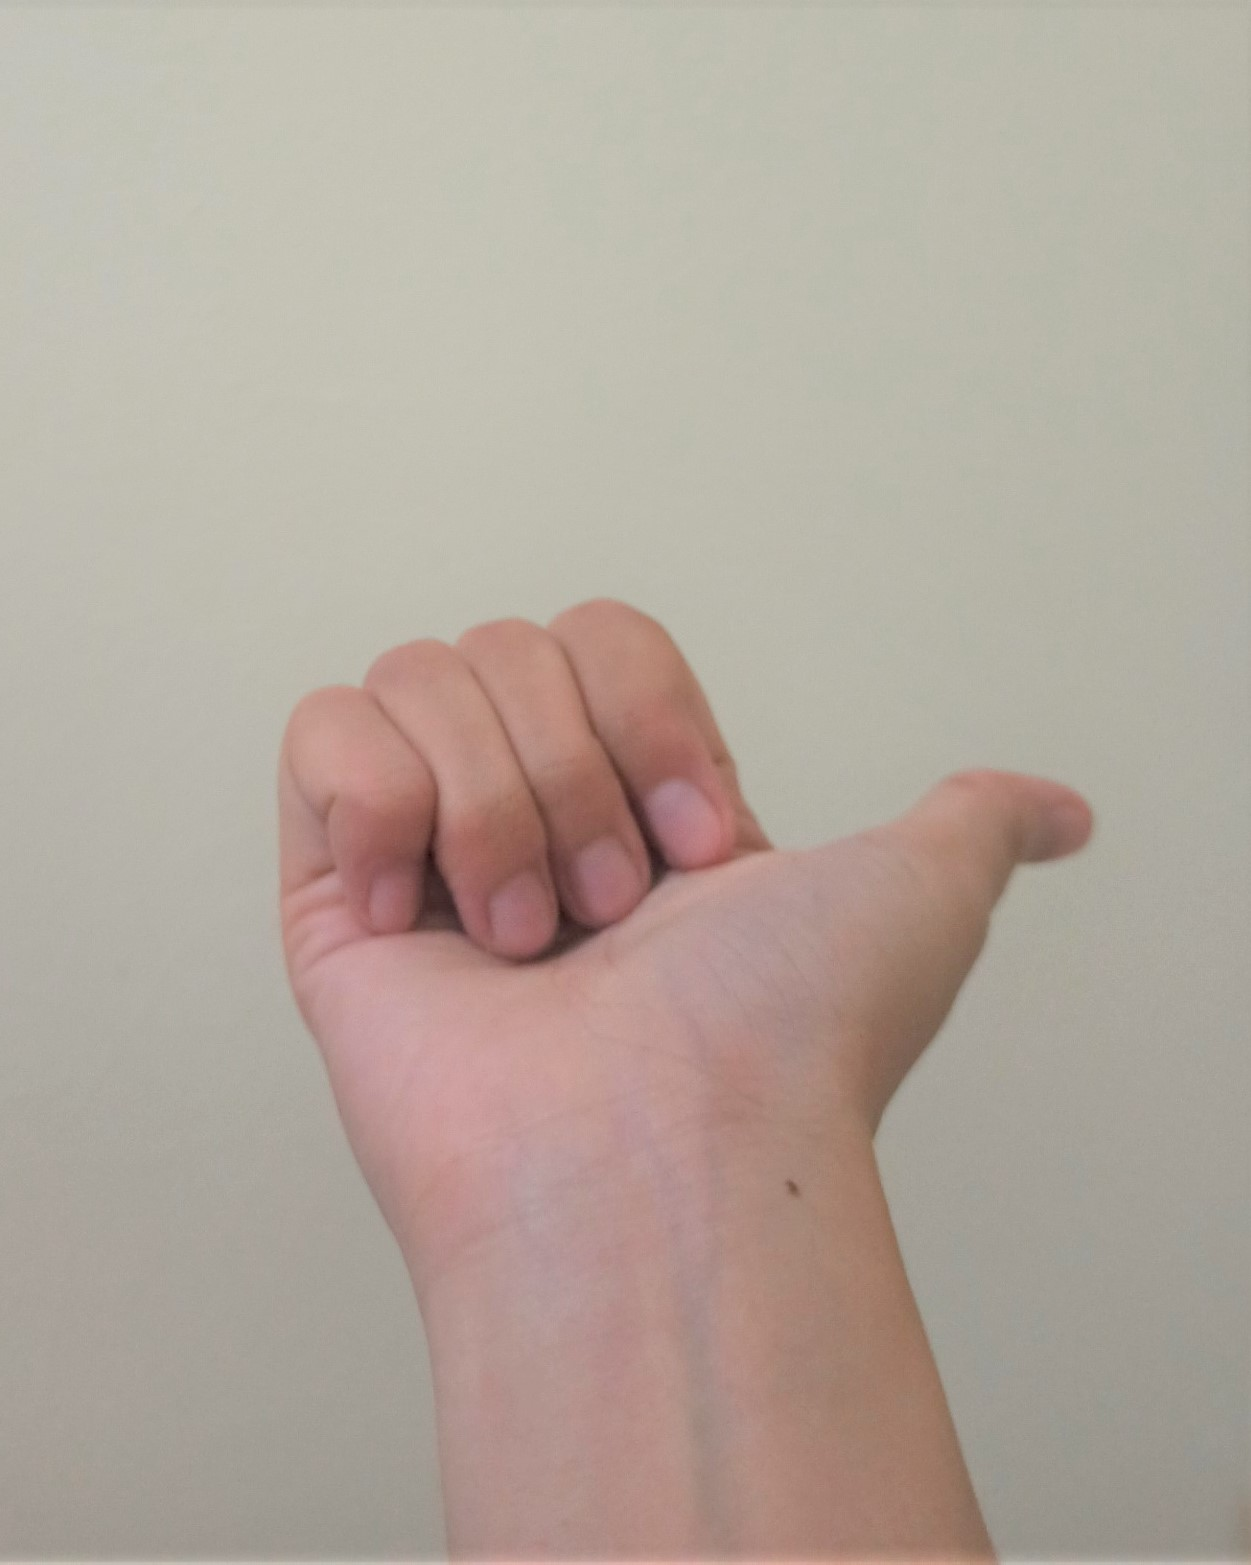
\includegraphics[width=\textwidth]{img/pola5b.jpg}
				\caption{\label{fig:gs5b}}
			\end{subfigure}
			\hspace{0.1em}
			\begin{subfigure}[t]{0.11\textwidth}
				\centering
				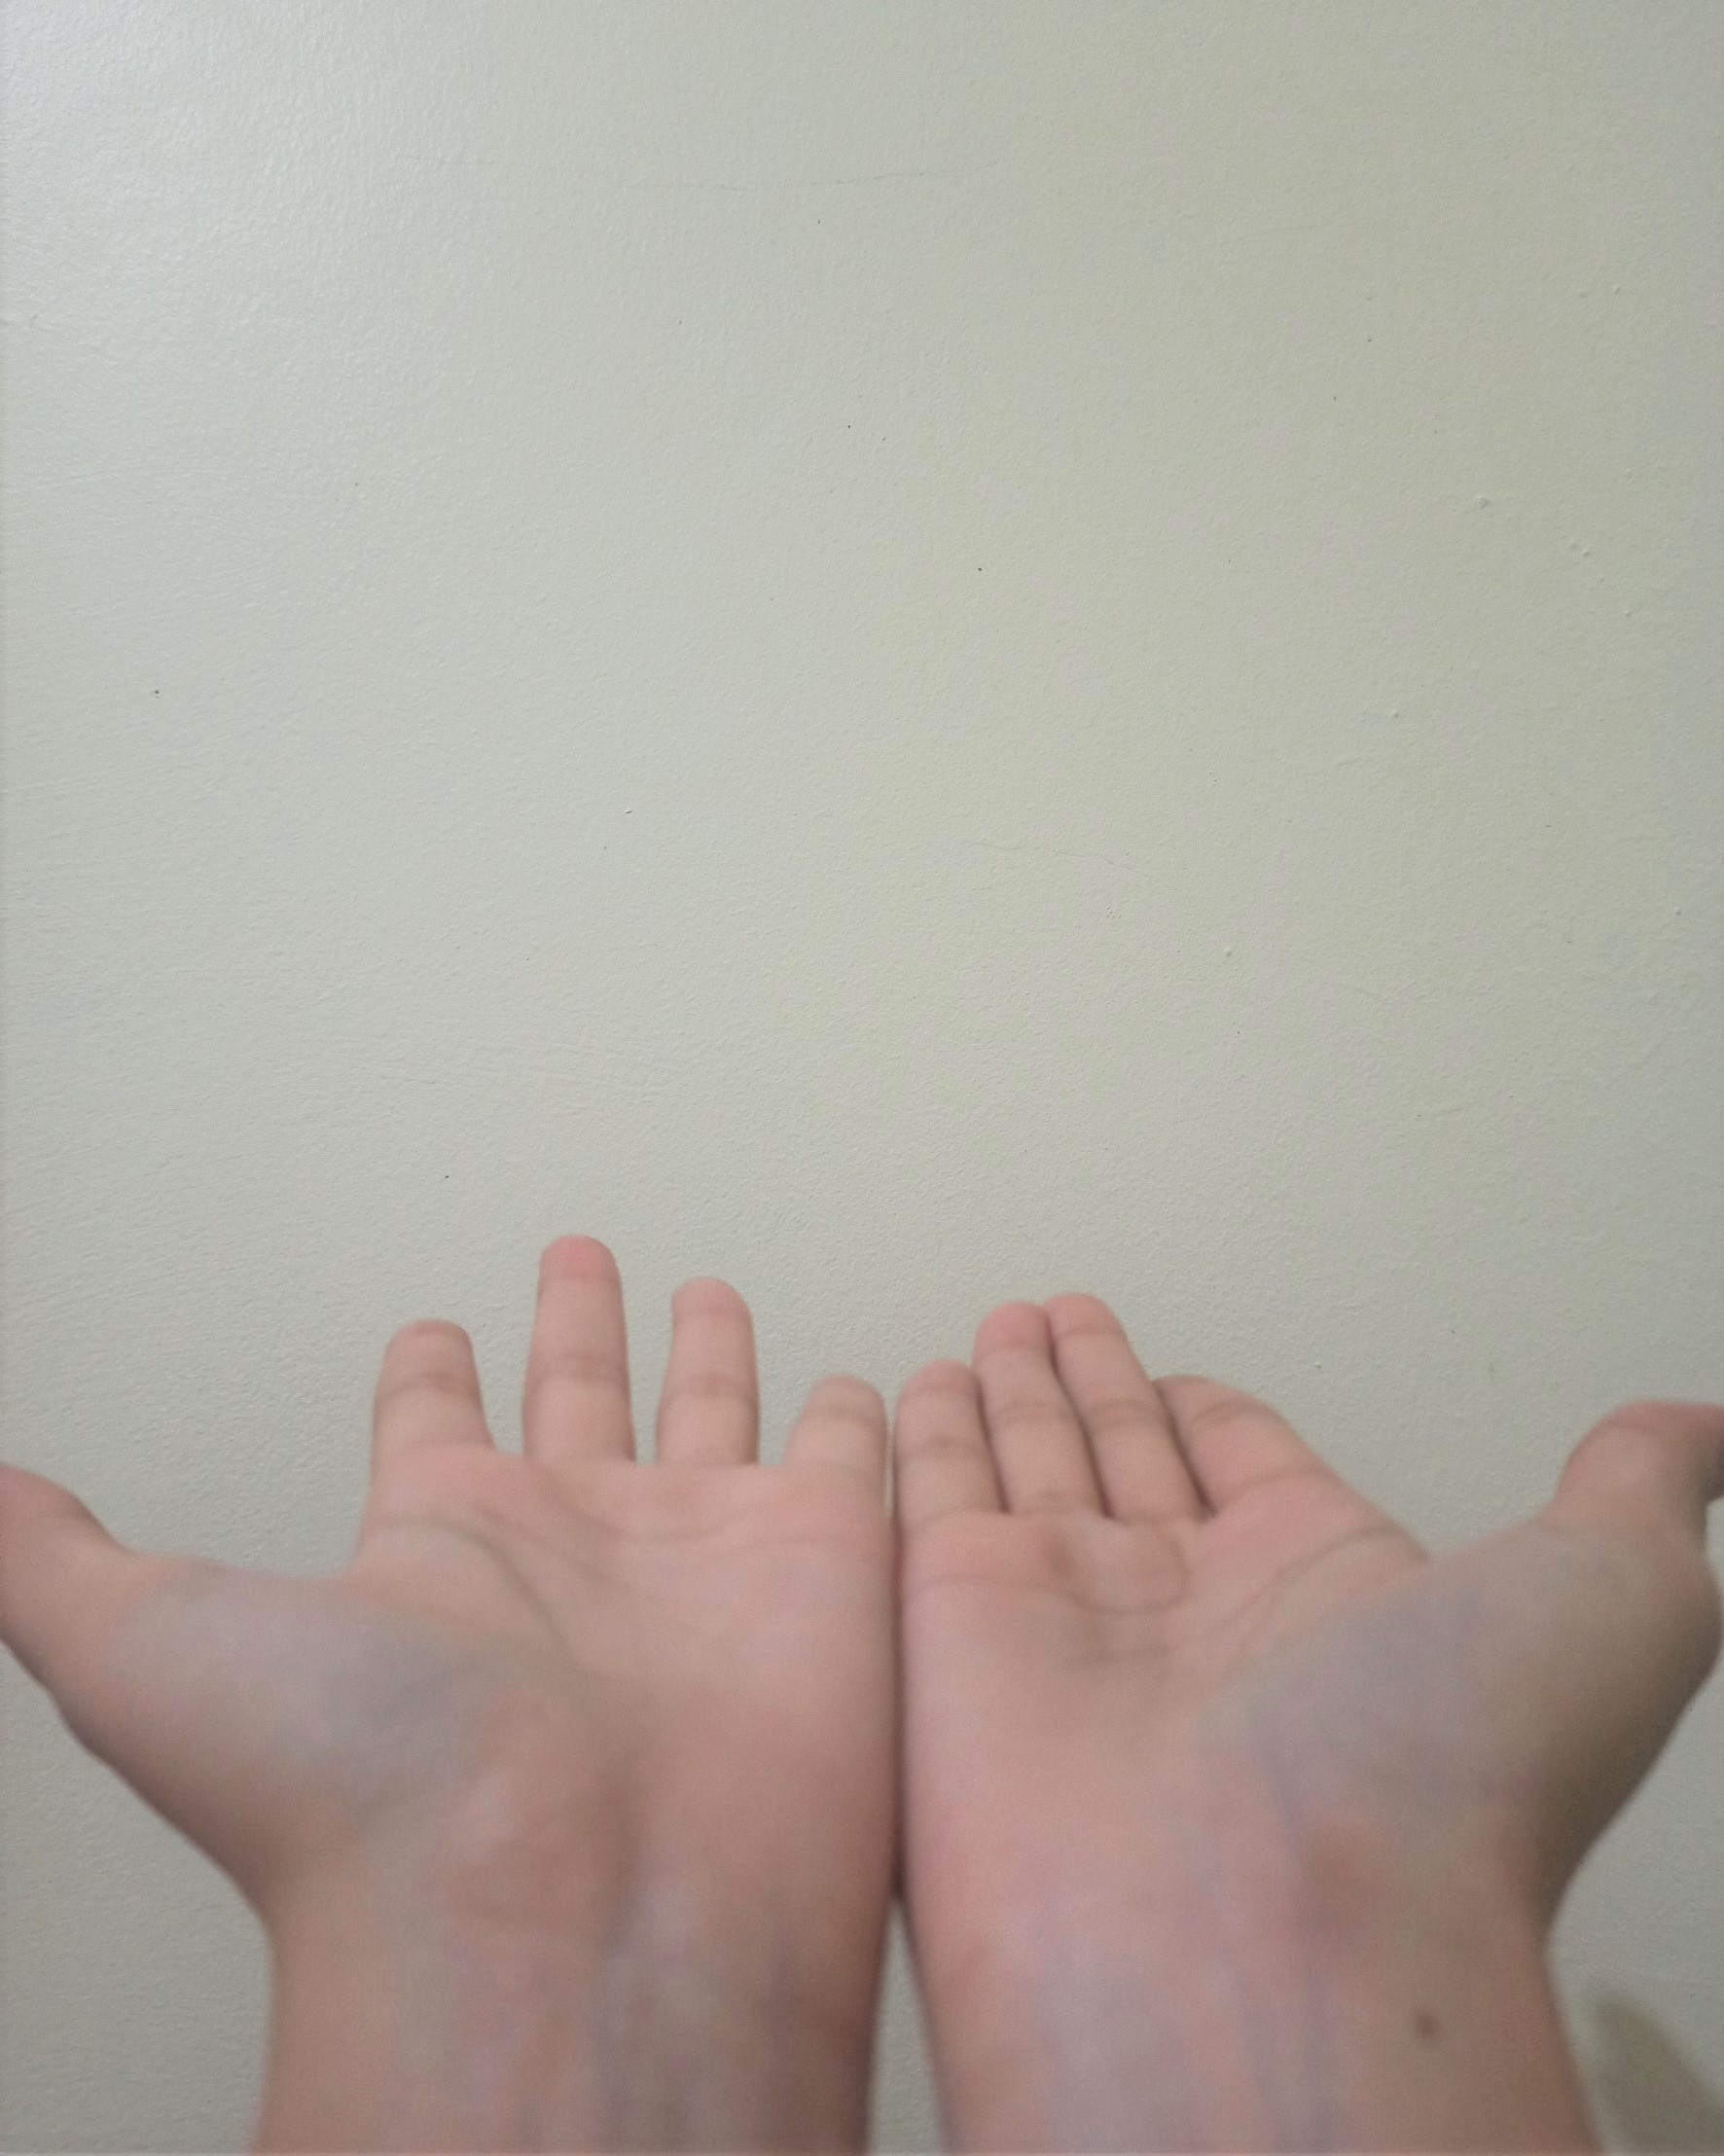
\includegraphics[width=\textwidth]{img/pola6.jpg}
				\caption{\label{fig:gs6}}
			\end{subfigure}
			\hspace{0.1em}
			\begin{subfigure}[t]{0.11\textwidth}
				\centering
				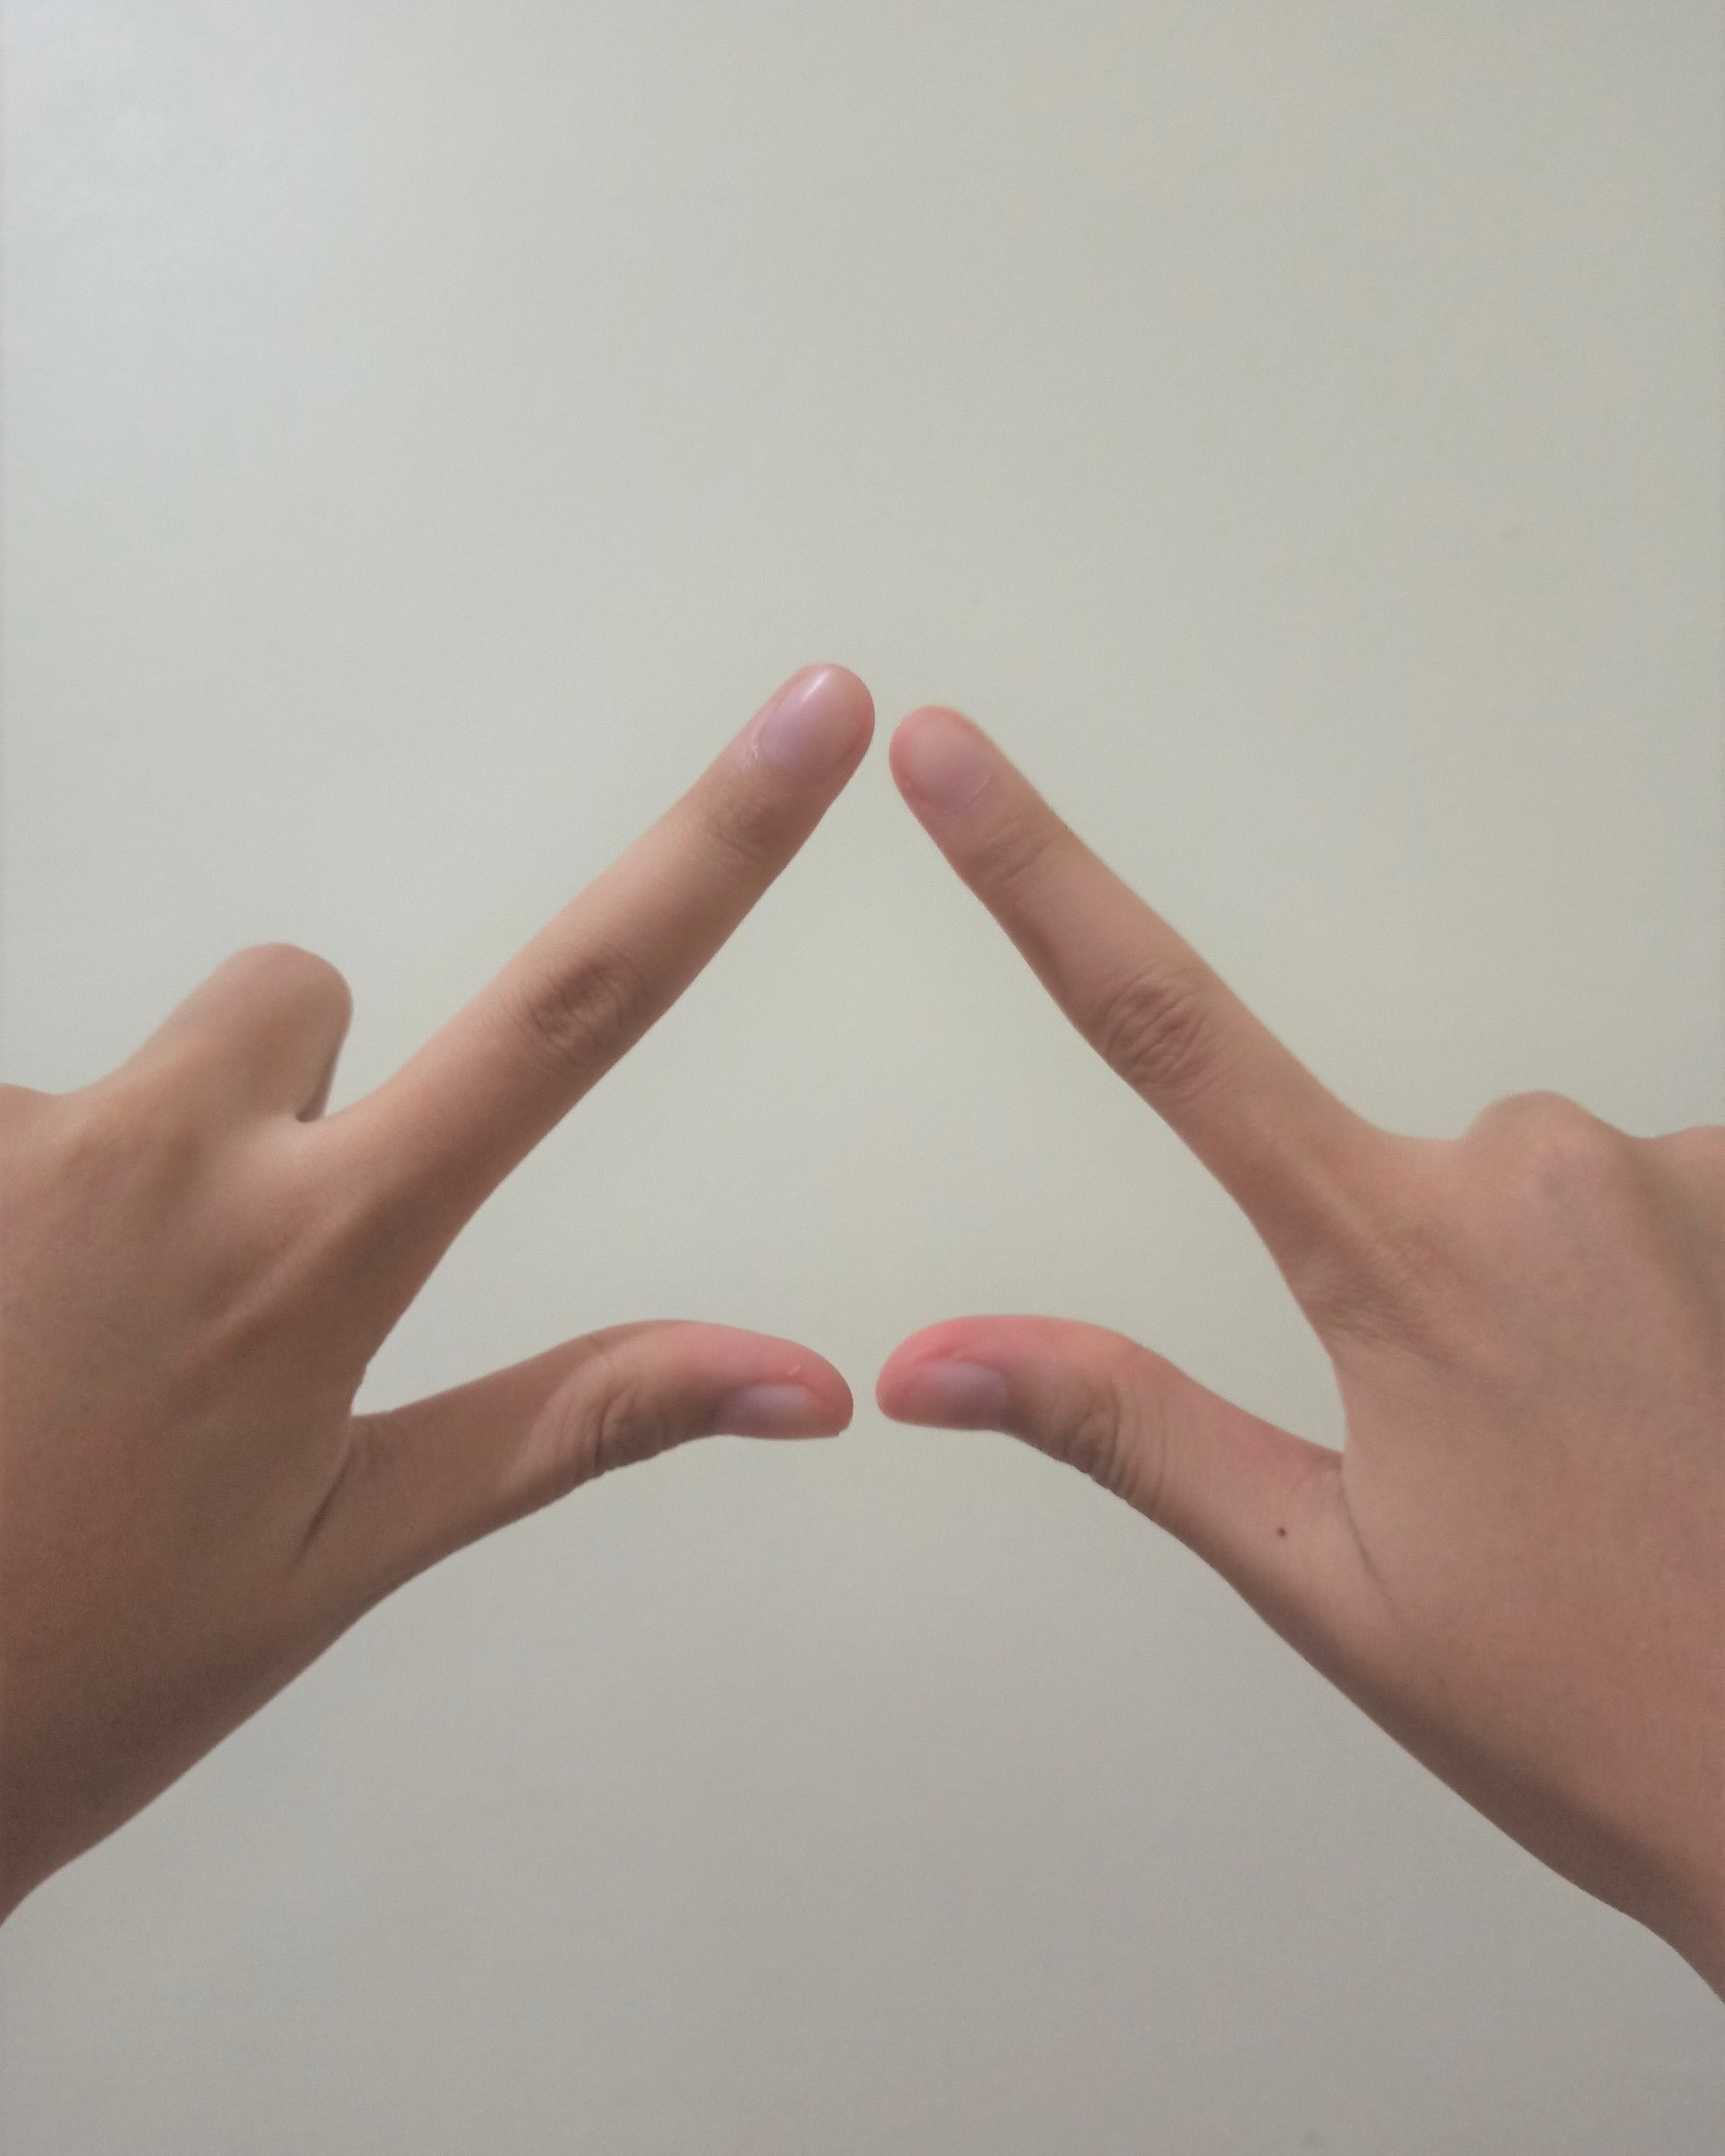
\includegraphics[width=\textwidth]{img/pola7.jpg}
				\caption{\label{fig:gs7}}
			\end{subfigure}
			\hspace{0.1em}
			\begin{subfigure}[t]{0.11\textwidth}
				\centering
				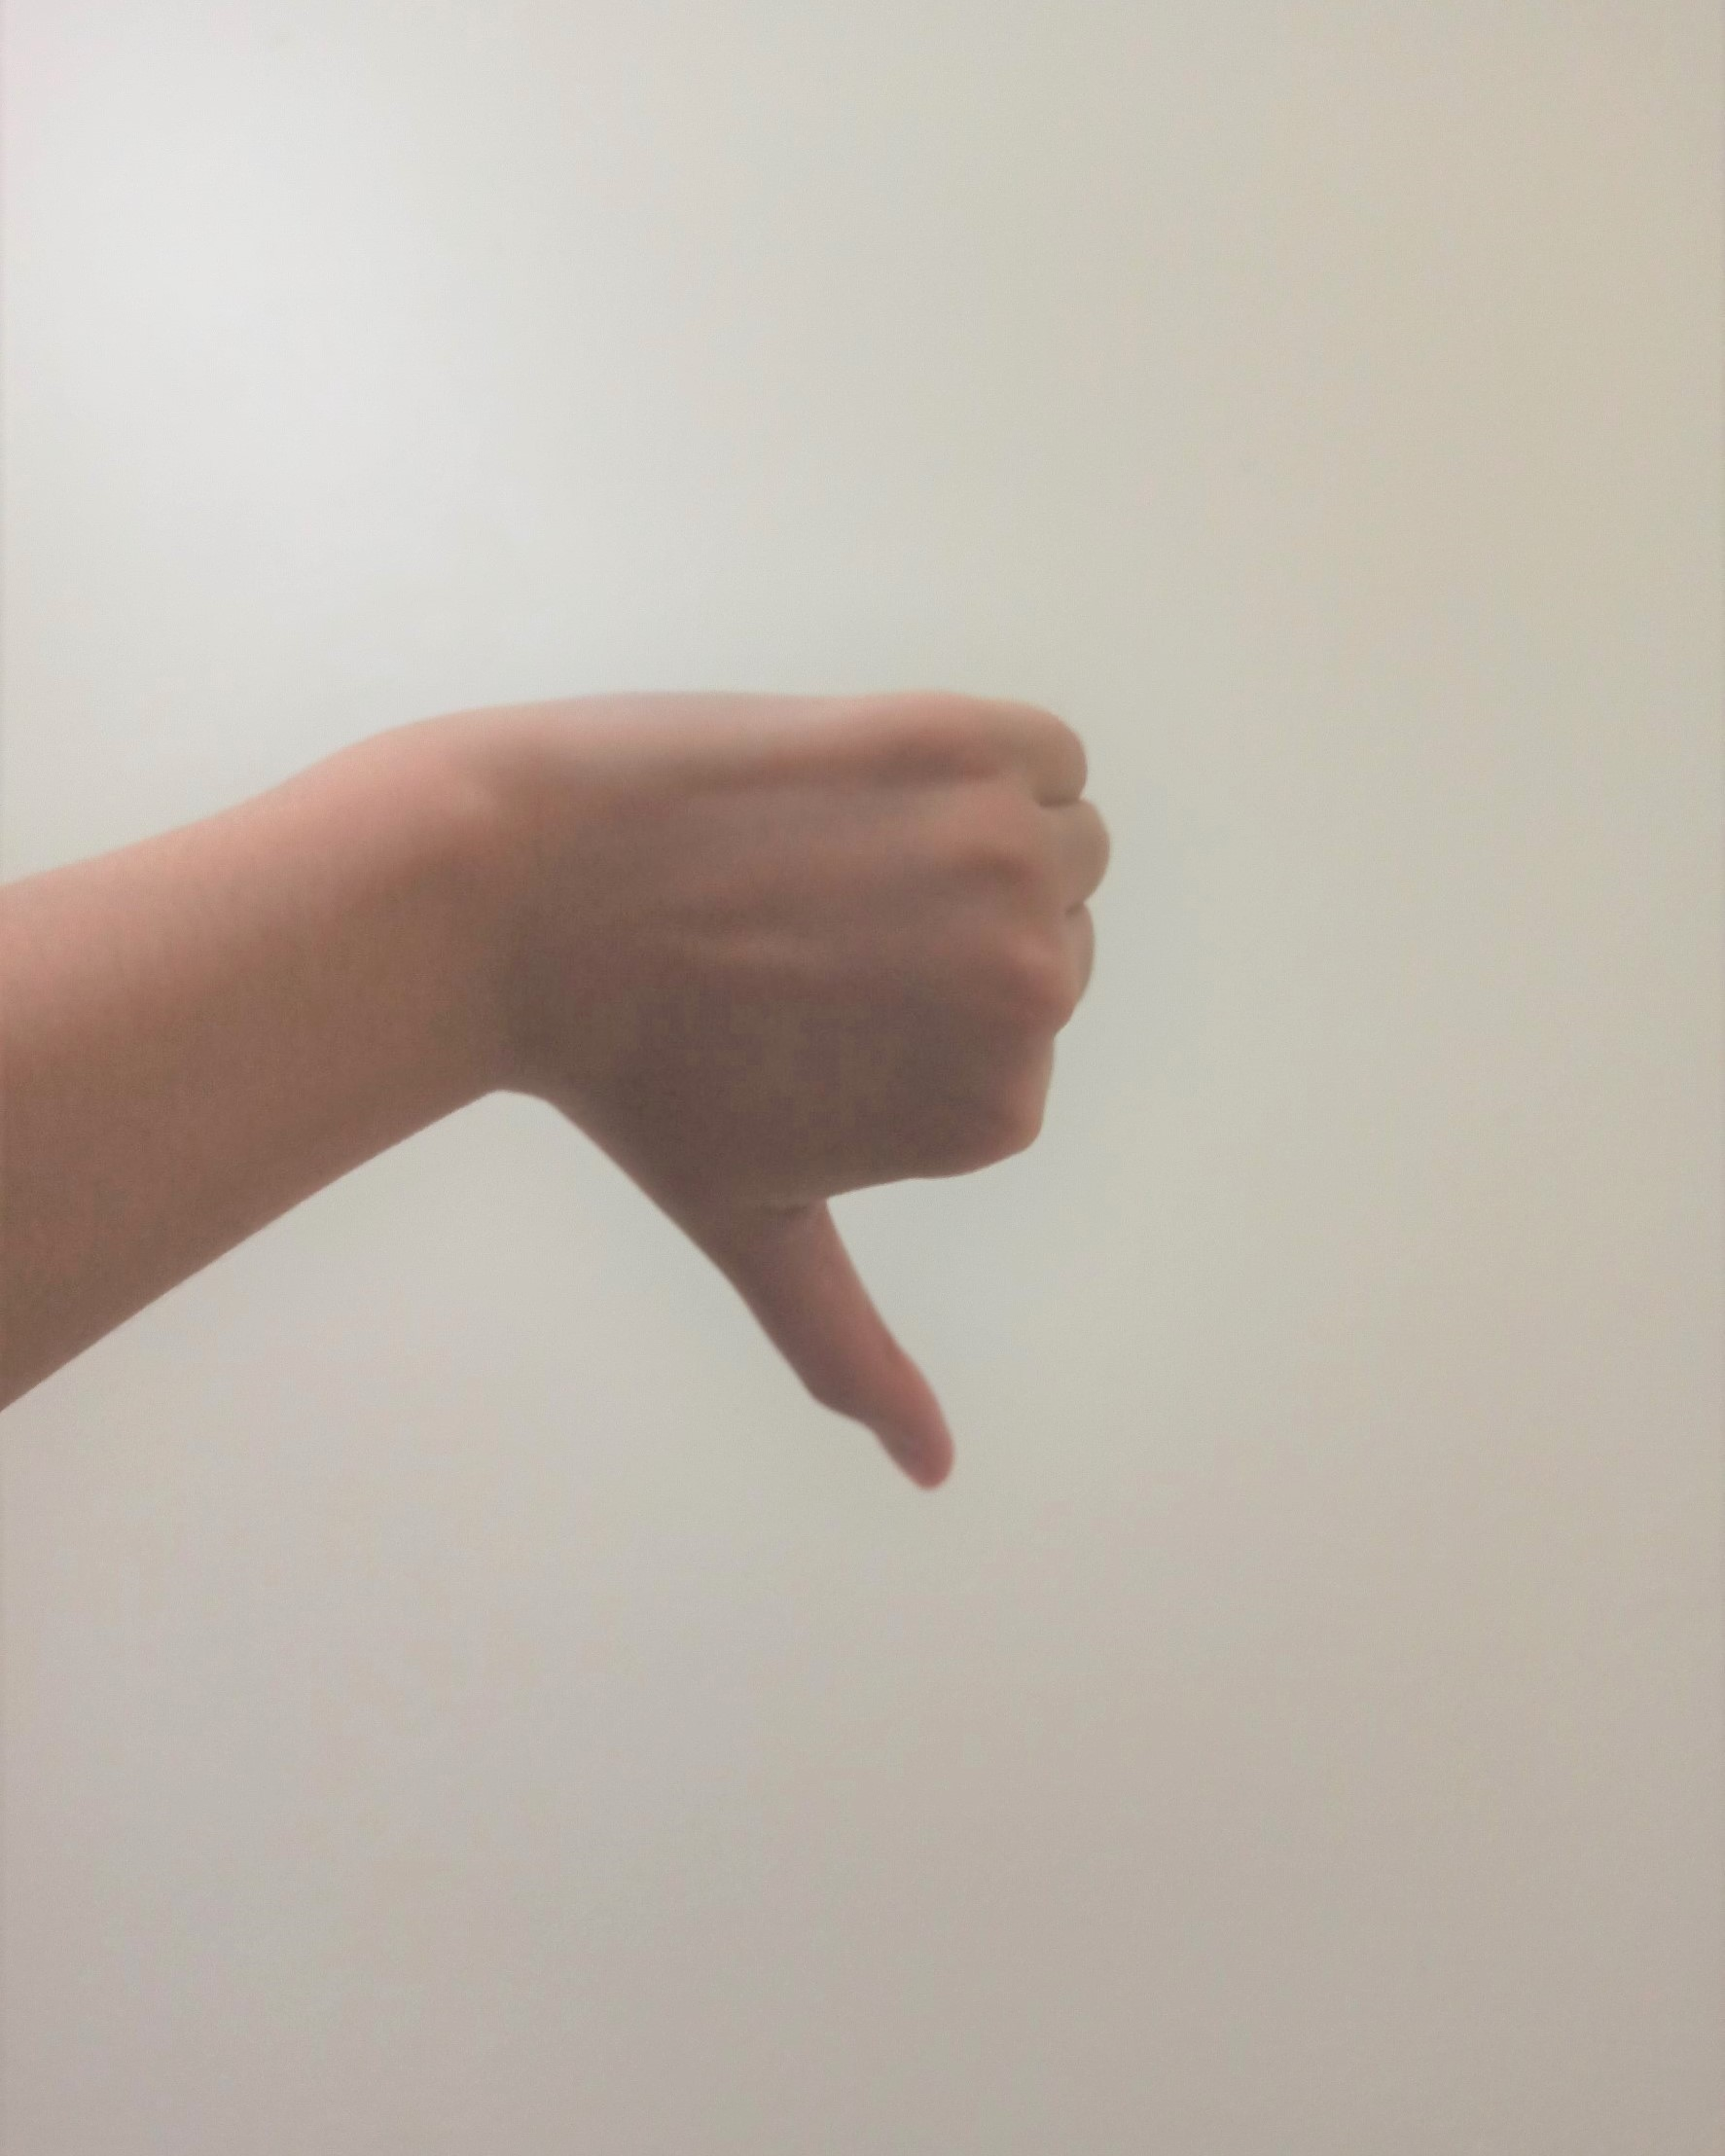
\includegraphics[width=\textwidth]{img/pola8a.jpg}
				\caption{\label{fig:gs8a}}
			\end{subfigure}
			\hspace{0.1em}
			\begin{subfigure}[t]{0.11\textwidth}
				\centering
				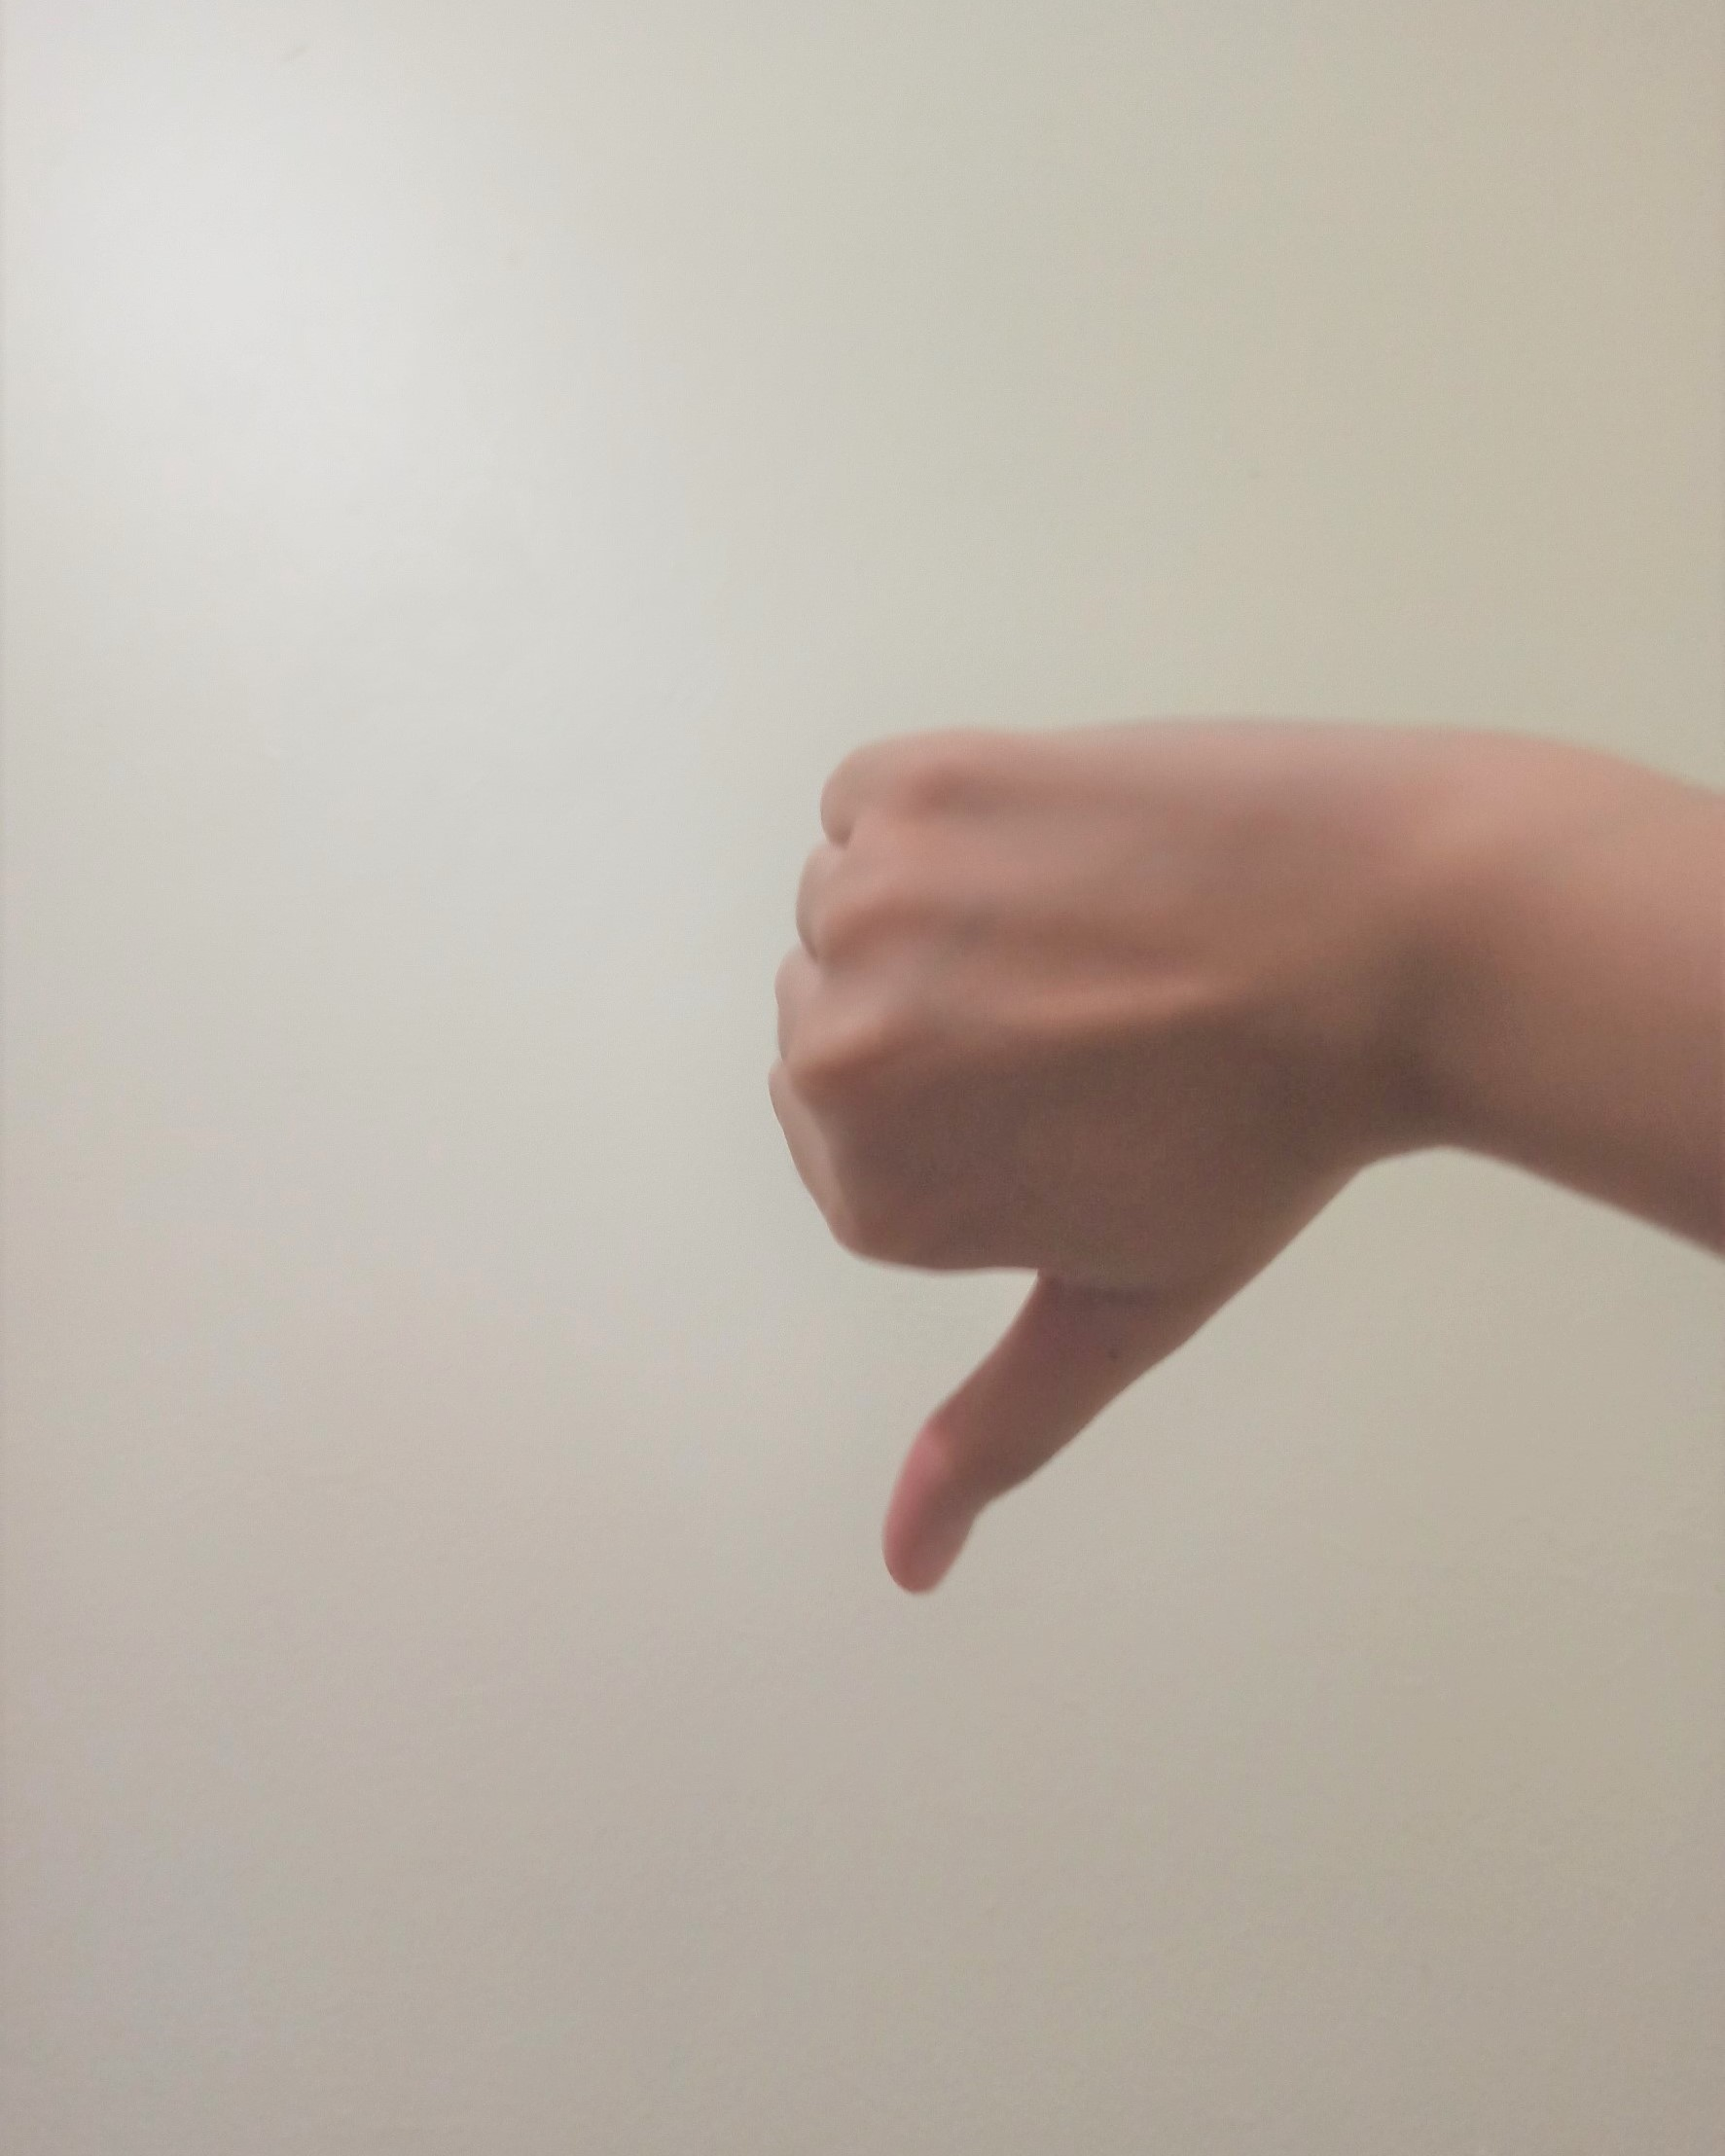
\includegraphics[width=\textwidth]{img/pola8b.jpg}
				\caption{\label{fig:gs8b}}
			\end{subfigure}
			\hspace{0.1em}
			\begin{subfigure}[t]{0.11\textwidth}
				\centering
				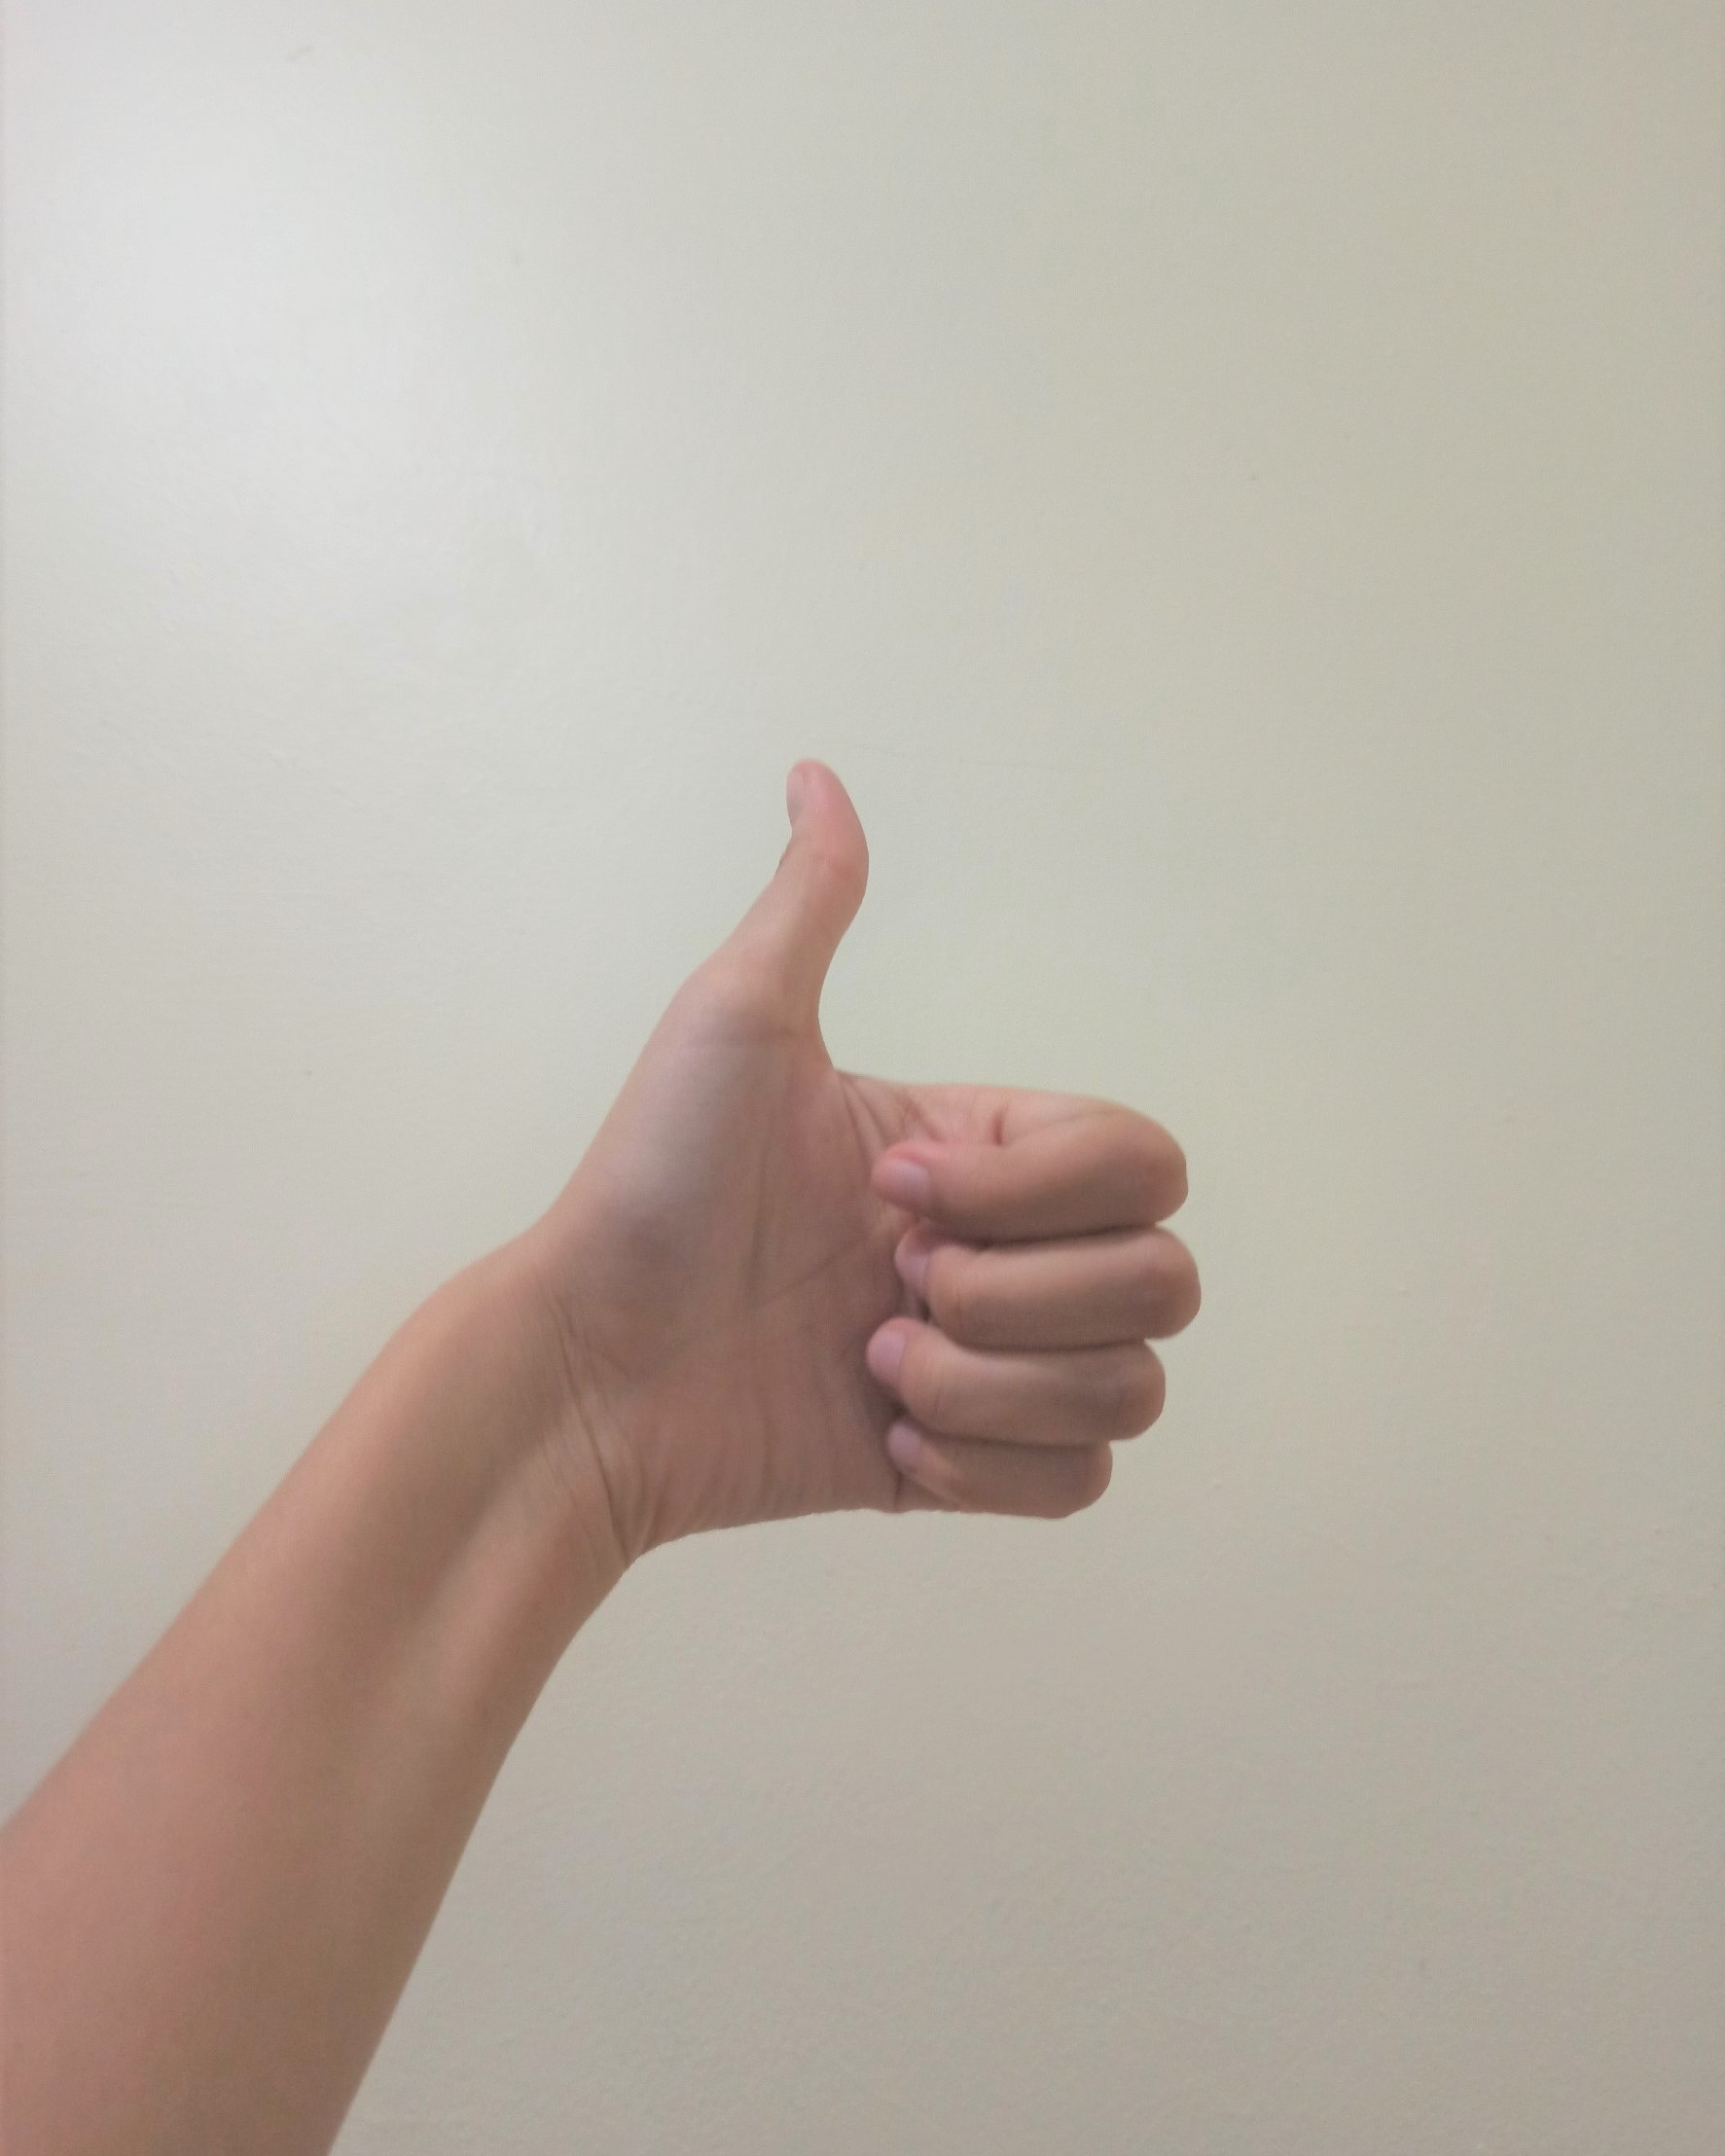
\includegraphics[width=\textwidth]{img/pola8c.jpg}
				\caption{\label{fig:gs8c}}
			\end{subfigure}
			\hspace{0.1em}
			\begin{subfigure}[t]{0.11\textwidth}
				\centering
				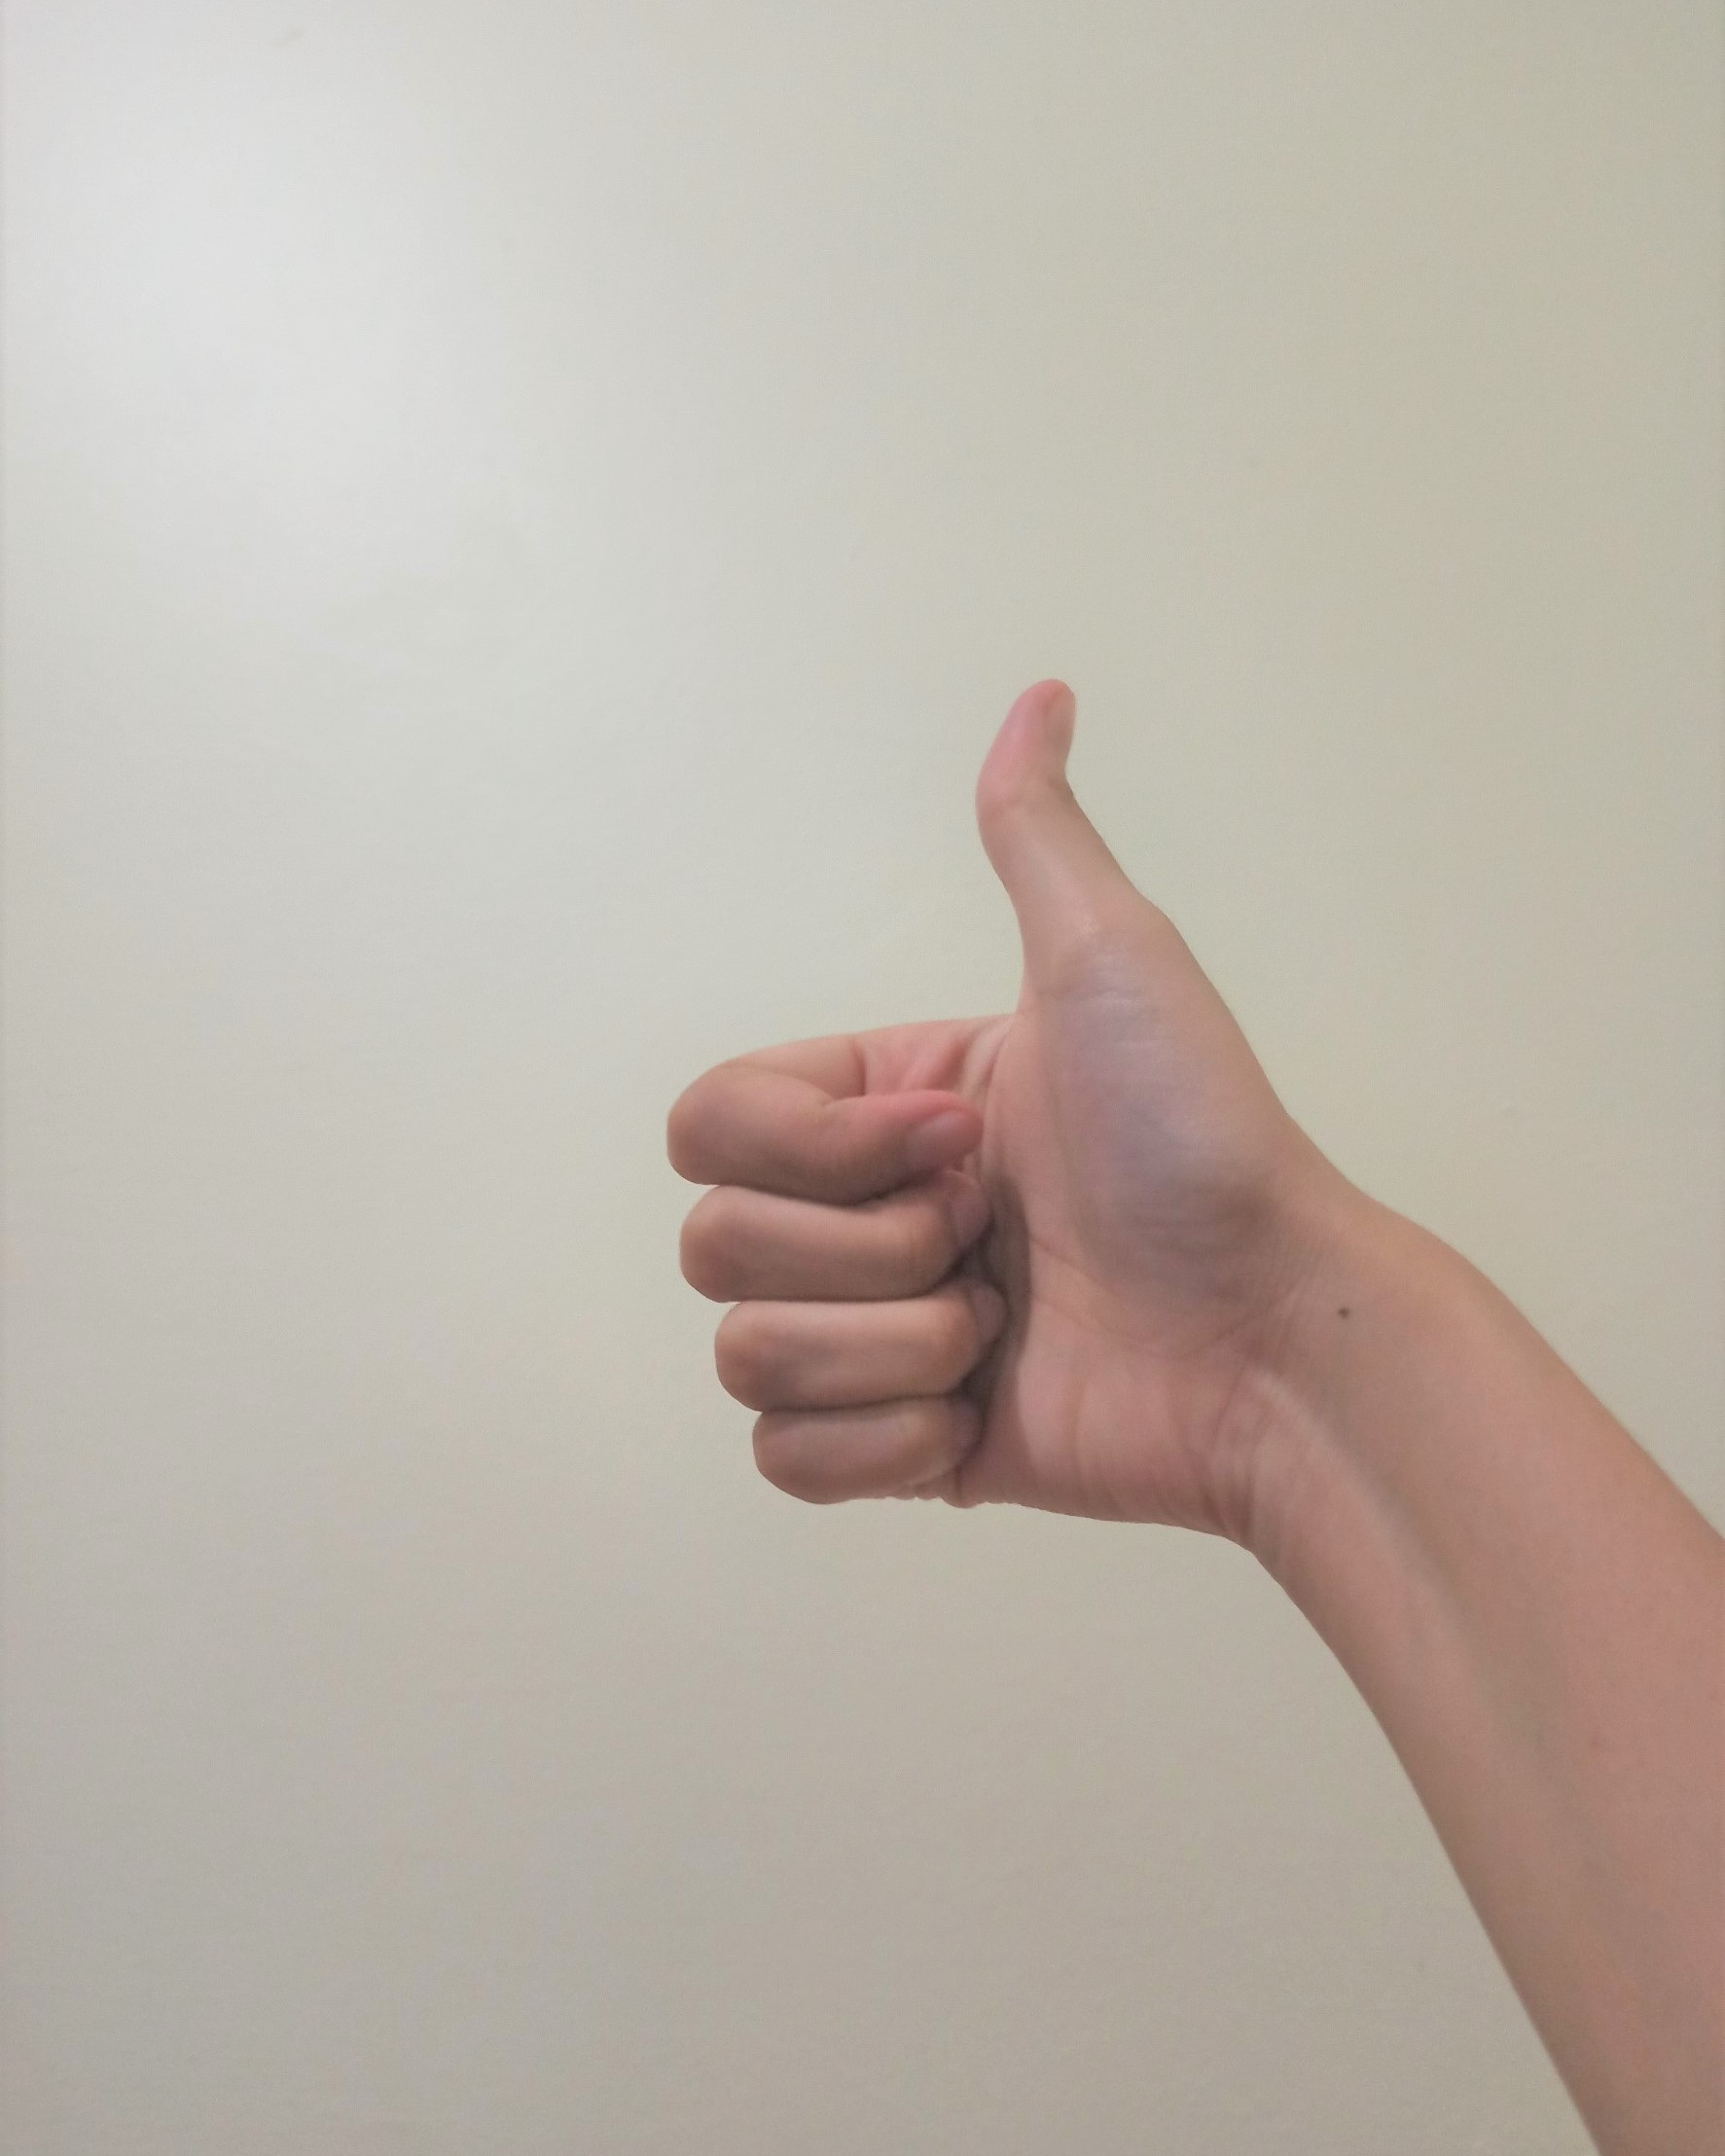
\includegraphics[width=\textwidth]{img/pola8d.jpg}
				\caption{\label{fig:gs8d}}
			\end{subfigure}
		\end{center}
			\vspace{-1ex}
			\caption{Gestur tangan yang pada sistem interaksi.}
			\label{fig:gestur_interaksi}
		\end{figure}

	
\section{PENGUJIAN DAN ANALISIS}
	\subsection{Pengujian Penyajian Objek Hologram} 
		\vspace{-2ex}
		\begin{figure} [h]
			\begin{center}
				\begin{subfigure}[t]{0.11\textwidth}
					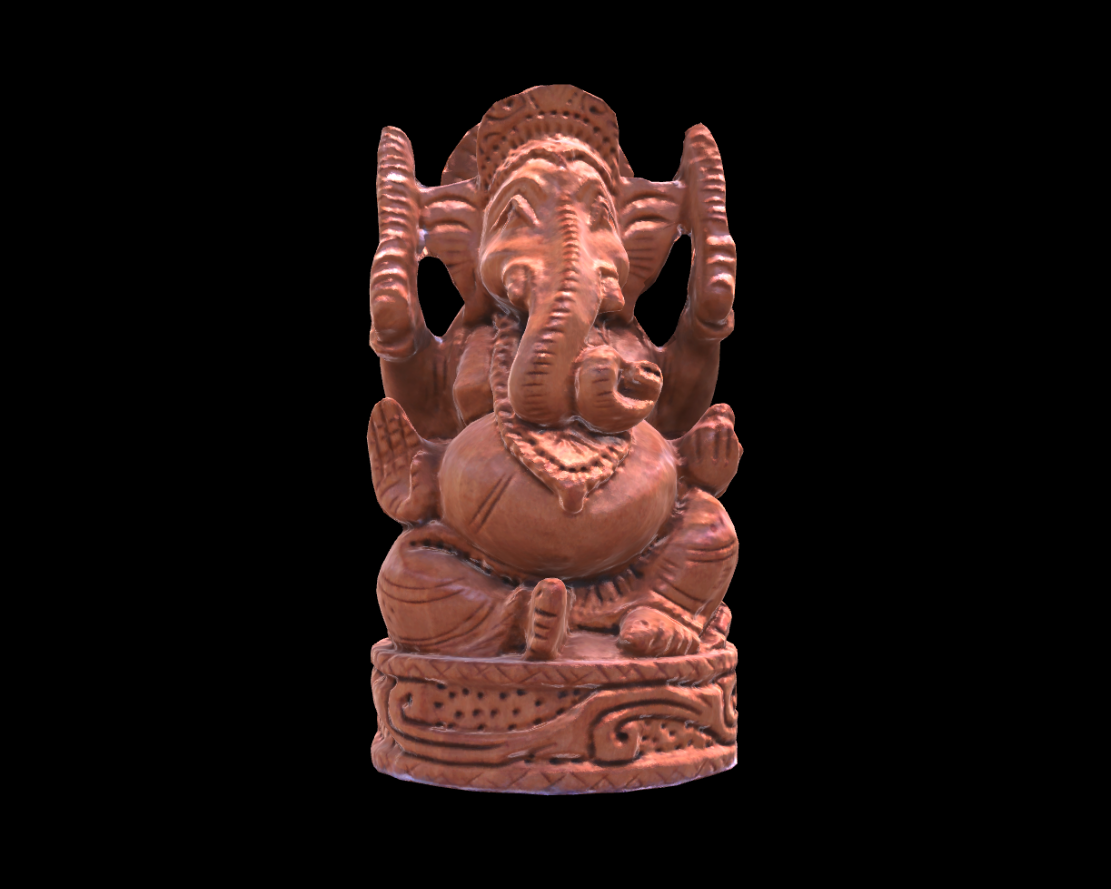
\includegraphics[width=\textwidth]{img/ilusi1.png}
					\caption{\label{fig:ilusi1}}
				\end{subfigure}
				\hspace{0.05em}
				\begin{subfigure}[t]{0.11\textwidth}
					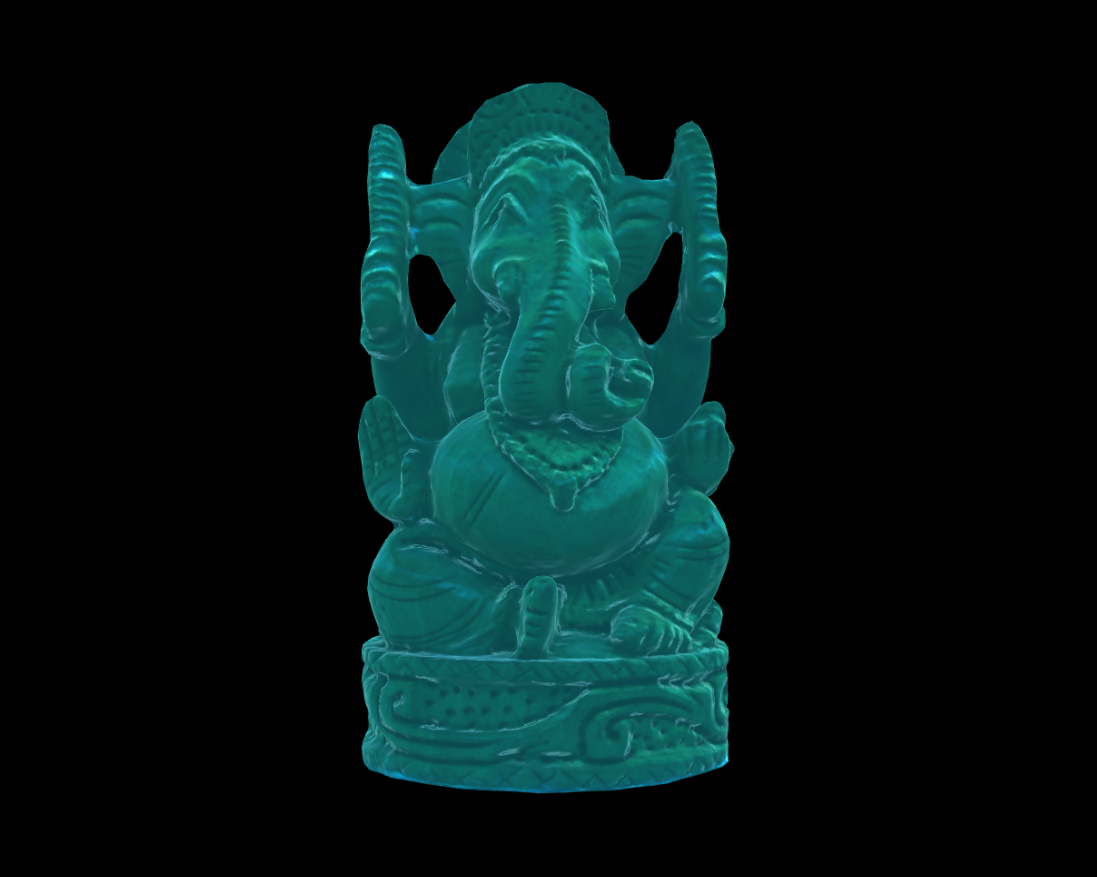
\includegraphics[width=\textwidth]{img/ilusi2.png}
					\caption{\label{fig:ilusi2}}
				\end{subfigure}
				\hspace{0.05em}
				\begin{subfigure}[t]{0.11\textwidth}
					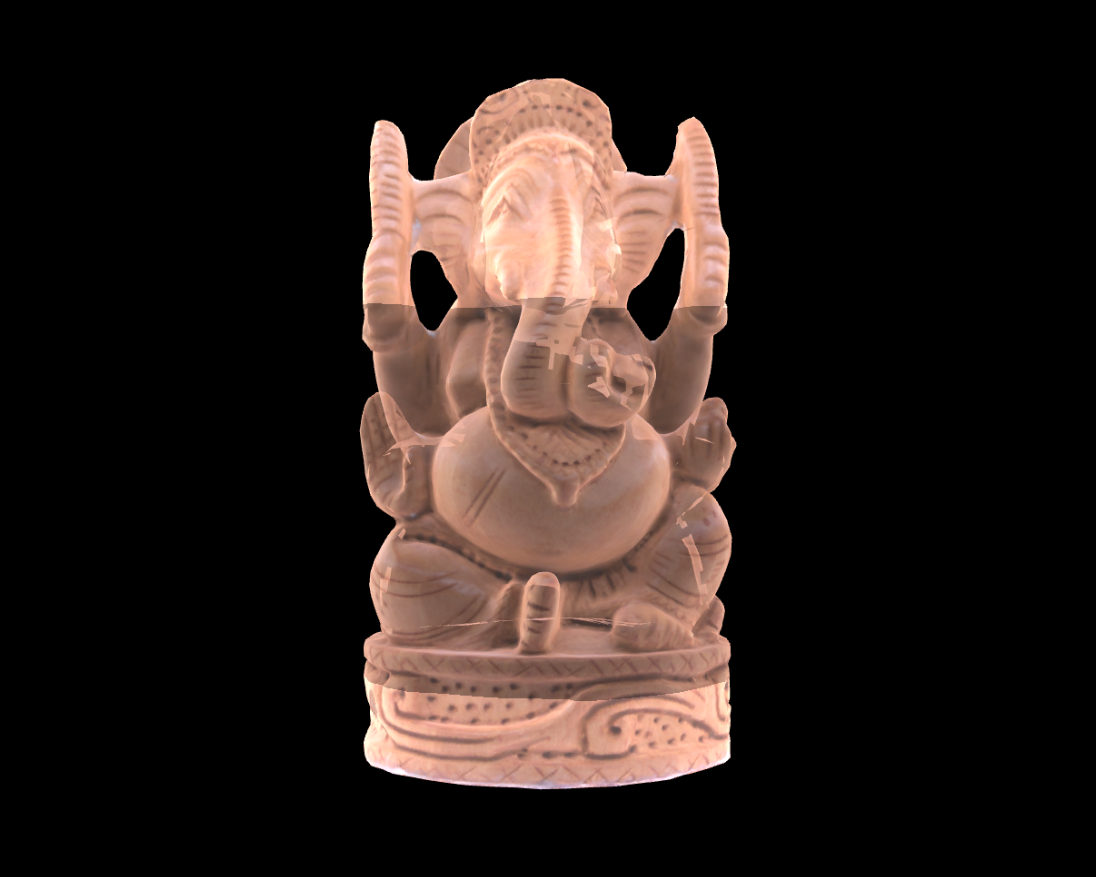
\includegraphics[width=\textwidth]{img/ilusi3.png}
					\caption{\label{fig:ilusi3}}
				\end{subfigure}
				\hspace{0.05em}
				\begin{subfigure}[t]{0.11\textwidth}
					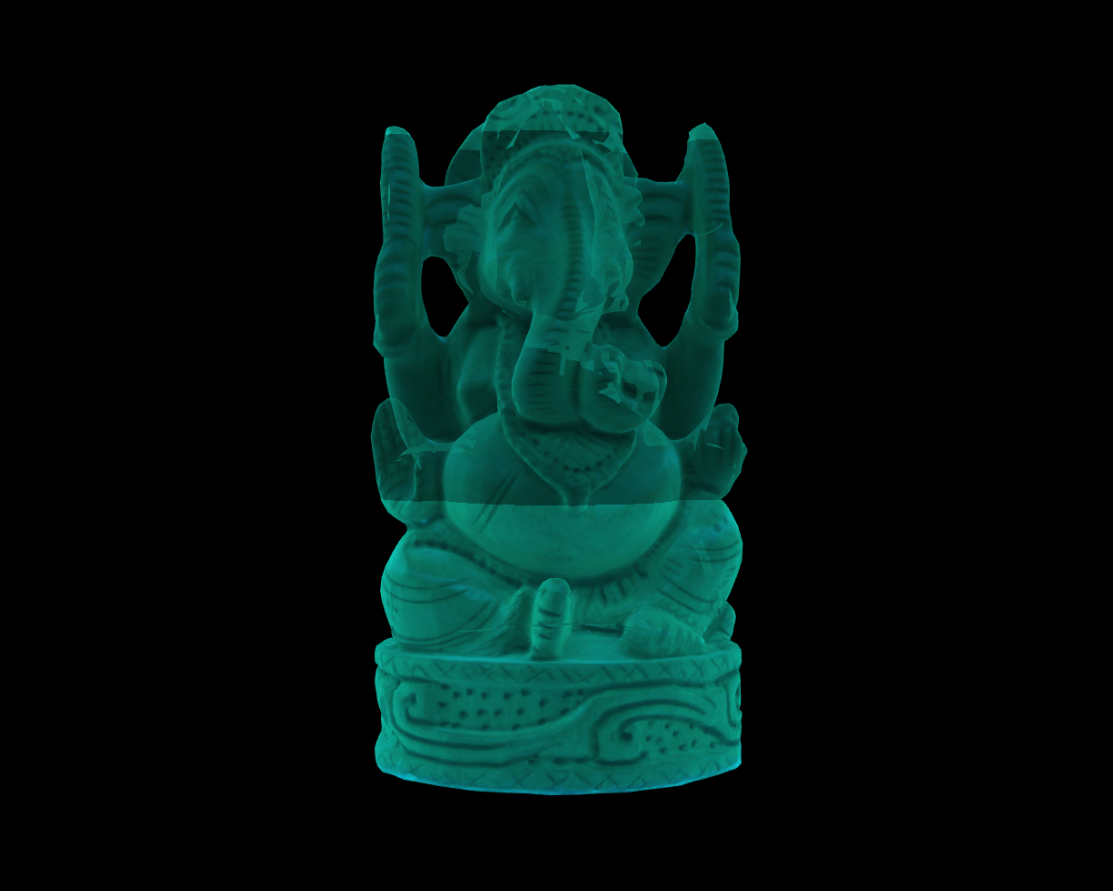
\includegraphics[width=\textwidth]{img/ilusi4.png}
					\caption{\label{fig:ilusi4}}
				\end{subfigure}
			\end{center}
			\vspace{-1ex}
			\caption{Perlakuan untuk efek hologram.}
			\label{fig:sb_p1}
		\end{figure}
		\vspace{-2ex}
	
		Pengujian ini bertujuan untuk mengetahui efek ilusi hologram manakah yang cocok diterapkan pada objek 3D yang akan diproyeksikan pada \textit{pyramid hologram}. Pengujian penyajian objek hologram dilakukan dengan memberikan 4 perlakuan yang berbeda pada setiap objek 3D dan menganalisa hasil proyeksinya sesuai pada gambar \ref{fig:sb_p1}. Pengujian dihitung dengan memberikan nilai untuk setiap perlakuan hologram terhadap masing-masing objek berdasarkan tingkat ketegasan objek hologram yang ditampilkan, dimana SB=3 poin, B=2 poin, KB=1 poin. Hasil pengujian dicantumkan pada tabel \ref{tab:hasil_penyajian}.
		
		\vspace{-1ex}
		\begin{table}[h]
			\caption{Hasil pengujian penyajian hologram.}
			\label{tab:hasil_penyajian}
			\vspace{-2ex}
			\begin{center}
			\begin{tabular}{|C{0.3cm}|L{2cm}|C{0.7cm}|C{0.7cm}|C{0.7cm}|C{0.7cm}|}
				\hline
				\multirow{2}{*}{\textbf{No}} & \multicolumn{1}{c|}{\multirow{2}{*}{\textbf{Objek}}} & \multicolumn{4}{c|}{\textbf{Efek Hologram (poin)}} \\ \cline{3-6}
				& \multicolumn{1}{c|}{}& \multicolumn{1}{c|}{\textbf{A}} & \multicolumn{1}{c|}{\textbf{B}} & \multicolumn{1}{c|}{\textbf{C}} & \multicolumn{1}{c|}{\textbf{D}} \\ \hline
				1.&\textit{Hand Axe}		& 3 & 1 & 2 & 1 \\ \hline
				2.&\textit{Primeval Axe}	& 2 & 1 & 3 & 1 \\ \hline
				3.&\textit{Buddha Statue}	& 2 & 1 & 3 & 2 \\ \hline
				4.&\textit{Ganesha Statue}	& 2 & 1 & 3 & 3 \\ \hline
				5.&\textit{Brass Lamp}		& 2 & 1 & 3 & 2 \\ \hline
				6.&\textit{Ceramic Pot}		& 3 & 1 & 3 & 1 \\ \hline
				7.&\textit{Typewriter}		& 3 & 1 & 3 & 1 \\ \hline
				8.&\textit{Gramophone}		& 2 & 1 & 2 & 1 \\ \hline
				\multicolumn{2}{|c|}{\textbf{Total}} & 19 & 8 & 22 & 12 \\ \hline
				\multicolumn{2}{|c|}{\textit{\textbf{Effectivity}}} & 79.16\% & 10.00\% & 91.67\% & 45.83\% \\ \hline
			\end{tabular}
			\end{center}
		\end{table}
		\vspace{-2ex}
		
		Dari hasil pengujian penyajian objek hologram didapatkan efek hologram dengan tingkat efektivitas tertinggi senilai 91.67\% pada efek hologram ketiga, yaitu kombinasi dari warna asli objek yang dapat memperlihatkan detail yang lebih baik dan cahaya semi-transparan yang memperlihatkan panjang, tinggi, dan lebar sebagai objek tiga dimensi yang bervolume.
		
	\subsection{Pengujian Deteksi Pengindera Tangan} 
		Pengujian deteksi pengindera tangan bertujuan untuk mengetahui kemampuan sistem dalam mengenali gestur tangan pengguna dan memberikan respons sesuai dengan fitur yang telah dirancang. Melalui pengujian ini, performansi pengindera tangan juga dapat diukur dengan memperhitungkan kemampuan baca bervariasi pola tangan. Berdasarkan 10 iterasi pengujian pada setiap gestur tangan sesuai gambar \ref{fig:gestur_interaksi}, didapatkan hasil sesuai tabel \ref{tab:hasil_deteksi}.
		
		\vspace{-1ex}
		\begin{table}[h]
			\caption{Hasil pengujian deteksi pengindera tangan.}
			\label{tab:hasil_deteksi}
			\begin{tabular}{|C{0.3cm}|m{2.8cm}|C{0.7cm}|C{0.7cm}|C{0.7cm}|C{0.7cm}|}
				\hline
				\multirow{2}{*}{\textbf{No}} & \multicolumn{1}{c|}{\multirow{2}{*}{\parbox{2.8cm}{\centering \textbf{Interaksi dan Pola Tangan}}}} & \multicolumn{3}{c|}{\textbf{Tangan (iterasi)}}&\multicolumn{1}{c|}{\textbf{Total}} \\ \cline{3-5}
				&& \textbf{Kiri} & \textbf{Kanan} & \textbf{Kedua} & \multicolumn{1}{c|}{}\\ \hline
				1.& Mengeksplorasi objek 		& 10 & 10 & -  & 20 \\ \hline
				2.& Memperbesar objek  			& -  & -  & 10 & 10	\\ \hline
				3.& Memperkecil objek  			& -  & -  & 10 & 10	\\ \hline
				4.& Mengaktifkan animasi 		& 9  & 9  & 10 & 28	\\ \hline
				5.& Mengembalikan objek 		& -  & -  & 9  & 9	\\ \hline
				6.& Menampilkan objek sebelumnya& 10 & -  & -  & 10 \\ \hline
				7.& Menampilkan objek setelahnya& -  & 10 & -  & 10	\\ \hline
				8.& Membuka Menu \textit{ Help}	& -  & -  & 8  & 8	\\ \hline
				9.& Membuka \textit{Main Menu}	& -  & -  & 8  & 8	\\ \hline
				10.& Membatalkan pilihan 		& 4  & 3  & -  & 7	\\ \hline
				11.& Menyetujui pilihan 		& 3  & 4  & -  & 7	\\ \hline			
				\multicolumn{2}{|c|}{\textbf{Total}}&36&36&55&127 \\ \hline
				\multicolumn{2}{|c|}{\textit{\textbf{Completion Rate}}}&72.00\%&72.00\%&97.50\% & 90.71\%\\ \hline
			\end{tabular}
		\end{table}
		\vspace{-2ex}
		
		Dari hasil pengujian deteksi pengindera tangan dengan total iterasi sebanyak 160 iterasi, didapatkan nilai sebesar 90.71\% gestur dapat dikenali oleh sistem dimana 72.00\% interaksi dapat dipicu oleh masing-masing tangan kiri dan tangan kanan serta sebesar 97.50\% keberhasilan oleh kedua tangan secara bersamaan (kanan dan kiri).
		
	\subsection{Pengujian Performansi Sistem}
		\label{section:p3}
		Pengujian performansi sistem bertujuan untuk mengetahui \textit{minumum requirement} yang dibutuhkan agar sistem dapat bekerja dengan cara \textit{server computer} dengan spesifikasi sesuai pada tabel \ref{tab:spesifikasi_pc}. Pengujian dilakukan sebanyak 5 kali iterasi pada tiap \textit{server computer} dengan skenario berupa mengeksplorasi masing-masing objek hologram yang ditampilkan, memutar objek, mengganti objek, dan menjalankan animasi. 
		\vspace{-1ex}
		\begin{table}[h]
			\caption{Spesifikasi \textit{server computer} pengujian performansi.}
			\label{tab:spesifikasi_pc}
			\vspace{-2ex}
			\begin{center}
				\begin{tabular}{|C{1.1cm}|C{2.25cm}|C{2.05cm}|C{1.7cm}|}
					\hline
					\textbf{Spesifikasi}  & \textbf{PC 1} 					& \textbf{PC 2}				& \textbf{PC 3} \\ \hline
					Nama Produk           & Asus ROG Strix G351GT			& Asus ROG Strix GL553VD	& Notebook Asus X450CP   \\ \hline
					\textit{Processor}    & Intel Core i7-9750H 			& Intel Core i7-7700HQ		& Intel Core i3-3217U     \\ \hline
					\textit{Graphic Card} & NVIDIA GeForce GTX 1650   		& NVIDIA GeForce GTX 1050	& AMD Radeon R5 M240    \\ \hline
					\textit{Storage Unit} & 512 GB SSD            			& 1TB HDD + 128 GB SSD		& 500 GB HDD     \\ \hline
					RAM                   & 16 GB							& 16 GB              		& 10 GB     \\ \hline
					Sistem Operasi        &	Windows 10 Home Edition 64-bit	& Windows 10 Education 64-bit & Windows 10 Pro 64-bit               \\ \hline
				\end{tabular}
			\end{center}
		\end{table}
		\vspace{-4ex}
		
		\begin{table}[h]
			\caption{Hasil pengujian performansi.}
			\vspace{-1ex}
			\begin{subtable}[t]{0.24\textwidth}
				\caption{\textit{Server computer} 1.}
				\label{tab:p3_pc1}
				\vspace{-2ex}
				\centering
				\begin{tabular}{|C{0.5cm}|C{0.5cm}|C{0.5cm}|C{0.5cm}|}
					\hline
					\multirow{2}{*}{\textbf{Itr.}} & \multicolumn{3}{c|}{\textit{\textbf{Frame Rate (fps)}}} \\ \cline{2-4} 
					& \textbf{Avg.}   & \textbf{Min.}  & \textbf{Max.}  \\ \hline
					1& 58.12 & 22.69 & 81.04 \\ \hline
					2& 55.81 & 24.65 & 76.98 \\ \hline
					3& 59.12 & 25.79 & 79.39 \\ \hline
					4& 54.84 & 24.64 & 81.64 \\ \hline
					5& 57.93 & 24.24 & 80.44 \\ \hline
				\end{tabular}
			\end{subtable}
			\begin{subtable}[t]{0.24\textwidth}
				\caption{\textit{Server computer} 2.}
				\label{tab:p3_pc2}
				\vspace{-2ex}
				\centering
				\begin{tabular}{|C{0.5cm}|C{0.5cm}|C{0.5cm}|C{0.5cm}|}
					\hline
					\multirow{2}{*}{\textbf{Itr.}} & \multicolumn{3}{c|}{\textit{\textbf{Frame Rate (fps)}}} \\ \cline{2-4} 
					& \textbf{Avg.}   & \textbf{Min.}  & \textbf{Max.}  \\ \hline
					1& 57.39 & 27.56 & 96.58 \\ \hline
					2& 57.87 & 30.48 & 88.19 \\ \hline
					3& 56.58 & 24.00 & 91.51 \\ \hline
					4& 57.57 & 21.64 & 88.89 \\ \hline
					5& 57.10 & 23.11 & 86.74 \\ \hline
				\end{tabular}
			\end{subtable}
			\begin{subtable}[t]{0.5\textwidth}
				\vspace{1ex}
				\caption{\textit{Server computer} 3.}
				\label{tab:p3_pc3}
				\vspace{-2ex}
				\centering
				\begin{tabular}{|C{0.5cm}|C{0.5cm}|C{0.5cm}|C{0.5cm}|}
					\hline
					\multirow{2}{*}{\textbf{Itr.}} & \multicolumn{3}{c|}{\textit{\textbf{Frame Rate (fps)}}} \\ \cline{2-4} 
					& \textbf{Avg.}   & \textbf{Min.}  & \textbf{Max.}  \\ \hline
					1& 45.73 & 11.71 & 66.95 \\ \hline
					2& 36.56 & 11.20 & 64.17 \\ \hline
					3& 43.82 & 11.54 & 65.86 \\ \hline
					4& 39.51 & 10.05 & 63.39 \\ \hline
					5& 38.27 & 10.29 & 61.50 \\ \hline
				\end{tabular}
			\end{subtable}
		\end{table}
		\vspace{-1ex}
		
		\subsubsection{Pengujian Performansi pada PC 1}
			 Hasil pengujian pada \textit{Server computer} 1 yang merupakan \textit{server} dengan spesifikasi tertinggi pada penelitian ini dicantumkan melalui tabel \ref{tab:p3_pc1}. Selisih antara nilai minimum dan maksimum setiap iterasi pun terhitung kecil dan stabil. Perubahan terbesar terjadi pada awal dan akhir sewaktu aplikasi dijalankan dikarenakan adanya peralihan \textit{game scene} ketika pengguna memasukin \textit{Main Scene} dan \textit{Main Menu}. Pada saat pengujian, perubahan \textit{frame} saat objek dieksplorasikan memperlihatkan pergerakan objek yang halus dan stabil.
		
		\subsubsection{Pengujian Performansi pada PC 2}
			Hasil pengujian pada \textit{server computer} 2 yang merupakan \textit{server} utama yang digunakan dalam pembuatan sistem \textit{interactive holographic projection} ditunjukkan melalui tabel \ref{tab:p3_pc2}. Di antara ketiga \textit{server computer} yang digunakan, PC 2 memiliki spesifikasi yang tidak jauh berbeda dengan PC 1. Hasil pengujian antara keduanya pun tidak jauh berbeda, secara umum pun pergerakan objek ketika dieksplorasikan terlihat cukup stabil meskipun tidak sebaik pada PC 1. Beberapa lonjakan \textit{frame rate} terjadi saat ada perubahan suatu gestur interaksi, seperti objek yang berhenti setelah aktivasi animasi objek selesai diputar. 
		
		\subsubsection{Pengujian Performansi pada PC 3}
			Hasil pengujian pada \textit{server computer} 3 yang merupakan \textit{server} dengan spesifikasi terendah pada penelitian ini ditunjukkan melalui tabel \ref{tab:p3_pc1}. Selisih antara nilai minimum dan maksimum antar iterasinya terhitung besar serta nilai rata-rata yang cenderung lebih rendah dibandingkan \textit{server computer} sebelumnya. Pergerakan objek terhadap gestur tangan yang diberikan terhitung kurang responsif dan terlihat loncatan pergerakan terhadap objek tersebut. Penggunaan PC 3 sebagai \textit{server computer} tidak dapat memaksimalkan kinerja sistem dengan baik dikarenakan daya komputasinya yang rendah.
			
		Dari hasil pengujian performansi sistem, sistem \textit{interactive holographic projection} dapat bekerja dengan baik seminimalnya pada \textit{computer server} dengan spesifikasi \textit{processor} Intel Core i7-7700HQ, \textit{graphic card} NVIDIA GeForce GTX 1050 dengan RAM sebesar 16 GB.
		
		
	\subsection{Pengujian Kebermanfaatan Sistem} 
		Pengujian kebermanfaatan sistem oleh pengguna bertujuan untuk mengevaluasi fungsi sistem secara keseluruhan (tanpa mengetaui detail sistem) dapat diterima oleh pengguna\cite{sawant2012software}.
	
		\subsubsection{Pengujian Efektivitas Sistem}
			\label{section:p4}
			Pengujian efektivitas sistem dilakukan dengan penggunaan sistem oleh 4 responden secara langsung. Responden diberikan 9 skenario yang terdiri dari 13 tugas mengenai keseluruhan sistem, dari penyajian hologram, interaksi gestur tangan, maupun \textit{interface} aplikasi, kemudian keberhasilannya tergantung dari banyaknya tugas yang sukses dilakukan. Hasil pengujian dicantumkan melalui tabel \ref{tab:hasil_efektivitas}.
			
			\vspace{-1ex}
			\begin{table}[h]
				\caption{Hasil pengujian efektivitas sistem.}
				\label{tab:hasil_efektivitas}
				\vspace{-2ex}
				\begin{center}
				\begin{tabular}{|C{0.4cm}|L{1.4cm}|C{0.7cm}|C{0.7cm}|C{0.7cm}|C{0.7cm}|C{0.7cm}|}
					\hline
					\multirow{2}{*}{\textbf{No}} & \multicolumn{1}{c|}{\multirow{2}{*}{\parbox{1.4cm}{\centering \textbf{Skenario Pengujian}}}} & \multicolumn{4}{c|}{\textbf{Responden (tugas)}}& \multicolumn{1}{c|}{\multirow{2}{*}{\textbf{Total}}} \\ \cline{3-6}
					& \multicolumn{1}{c|}{}& \multicolumn{1}{c|}{\textbf{A}} & \multicolumn{1}{c|}{\textbf{B}} & \multicolumn{1}{c|}{\textbf{C}} & \multicolumn{1}{c|}{\textbf{D}} & \multicolumn{1}{c|}{}\\ \hline
					1.&Skenario 1 & 1 & 1 & 1 & 1 & 4  \\ \hline
					2.&Skenario 2 & 1 & 1 & 1 & 1 & 4  \\ \hline
					3.&Skenario 3 & 8 & 8 & 8 & 8 & 32 \\ \hline
					4.&Skenario 4 & 2 & 2 & 2 & 2 & 8 \\ \hline
					5.&Skenario 5 & 2 & 2 & 2 & 2 & 8 \\ \hline
					6.&Skenario 6 & 2 & 2 & 2 & 2 & 8 \\ \hline
					7.&Skenario 7 & 2 & 1 & 2 & 2 & 7 \\ \hline
					8.&Skenario 8 & 1 & 1 & 1 & 1 & 4 \\ \hline
					9.&Skenario 9 & 1 & 0 & 1 & 1 & 3 \\ \hline
					10.&Skenario 10 & 0 & 0 & 1 & 1 & 2 \\ \hline
					11.&Skenario 11 & 1 & 0 & 2 & 0 & 3 \\ \hline
					12.&Skenario 12 & 0 & 0 & 1 & 0 & 1 \\ \hline
					13.&Skenario 13 & 1 & 0 & 1 & 1 & 3 \\ \hline
					\multicolumn{2}{|c|}{\textbf{Total}} & 22 & 18 & 25 & 22 & 87 \\ \hline
					\multicolumn{2}{|c|}{\textit{\textbf{Completion Rate}}} & 88.0\% & 72.0\% & 100\% & 88.0\% & 87.0\% \\ \hline
				\end{tabular}
				\end{center}
			\end{table}
			\vspace{-2ex}
			
			Dari hasil pengujian efektivitas sistem dengan \textit{completion rate} sebesar 87.0\%, 87 tugas yang dilakukan responden dapat direspons balik oleh sistem sesuai dengan fitur yang dibangun. Sedangkan 12 tugas lainnya tidak dapat memberikan respons yang bersesuaian dikarenakan detektor gestur harus mengenali posisi \textit{hand object} dengan tepat (terlalu sensitif). 

		\subsubsection{Pengujian Kepuasan Pengguna} 		
			Pengujian kepuasan pengguna dilakukan dengan cara menyebarkan kuesioner daring yang dilengkapi dengan video skenario. Pada pengujian kuesioner ini, 61 responden diberikan 30 pernyataan untuk mengetahui tingkat persetujuannya sesuai dengan opsi sangat setuju (SS), setuju (S), netral (N), tidak setuju (ST), dan sangat tidak setuju (STS). Hasil pengujian dicantumkan pada tabel \ref{tab:hasil_kepuasan}.
			
			\vspace{-1ex}
			\begin{table}[h]
				\caption{Hasil pengujian kepuasan pengguna.}
				\label{tab:hasil_kepuasan}
				\vspace{-2ex}
				\begin{center}
				\begin{tabular}{|l|C{0.7cm}|C{0.7cm}|C{0.7cm}|C{0.7cm}|C{0.7cm}|}
				\hline
				\multicolumn{1}{|c|}{\multirow{2}{*}{\textbf{Pernyataan}}} & \multicolumn{5}{c|}{\textbf{Jawaban}} \\ \cline{2-6} 
				\multicolumn{1}{|c|}{}	& \textbf{STS} 	 & \textbf{TS}	  & \textbf{N}	  & \textbf{S}		& \textbf{SS}     \\ \hline
				Pernyataan 1 & 37.7\% & 0\%    & 0\%    & 0\%  	& 62.3\% \\ \hline
				Pernyataan 2 & 32.8\% & 0\%    & 0\%    & 0\%  	& 67.2\% \\ \hline
				Pernyataan 3 & 39.3\% & 0\%    & 0\%    & 0\% 	& 60.7\% \\ \hline
				Pernyataan 4 & 0\%	 & 4.9\%  & 29.5\% & 55.7\%	& 9.8\%  \\ \hline
				Pernyataan 5 & 0\%	 & 1.6\%  & 23\%   & 45.9\% & 29.5\% \\ \hline
				Pernyataan 6 & 0\%	 & 6.6\%  & 21.3\% & 44.3\%	& 27.9\% \\ \hline
				Pernyataan 7 & 1.6\%  & 19.7\% & 32.8\% & 37.7\% & 8.2\%  \\ \hline
				Pernyataan 8 & 1.6\%  & 9.8\%  & 34.4\% & 31.1\% & 23\%   \\ \hline
				Pernyataan 9 & 0\%	 & 6.6\%  & 18\%   & 54.1\% & 21.3\% \\ \hline
				Pernyataan 10 & 1.6\%  & 13.1\% & 34.4\% & 39.3\% & 11.5\% \\ \hline
				Pernyataan 11 & 0\%	 & 0\% 	  & 9.8\%  & 41\%   & 49.2\% \\ \hline
				Pernyataan 12 & 0\%	 & 0\%	  & 6.6\%  & 42.6\% & 50.8\% \\ \hline
				Pernyataan 13 & 0\%	 & 4.9\%  & 16.4\% & 44.3\% & 34.4\% \\ \hline
				Pernyataan 14 & 0\%	 & 0\% 	  & 8.2\%  & 41\%	& 50.8\% \\ \hline
				Pernyataan 15 & 0\%	 & 0\%    & 11.5\% & 45.9\% & 42.6\% \\ \hline
				Pernyataan 16 & 0\%	 & 1.6\%  & 14.8\% & 41\%	& 42.6\% \\ \hline
				Pernyataan 17 & 0\%	 & 1.6\%  & 11.5\% & 37.7\% & 49.2\% \\ \hline
				Pernyataan 18 & 0\%	 & 3.3\%  & 16.4\% & 55.7\% & 24.6\% \\ \hline
				Pernyataan 19 & 0\%    & 3.3\%  & 9.8\%  & 32.8\% & 54.1\% \\ \hline
				Pernyataan 20 & 0\%    & 0\% 	  & 13.1\% & 31.1\% & 55.7\% \\ \hline
				Pernyataan 21 & 0\%    & 1.6\%  & 8.2\%  & 31.1\% & 59\%   \\ \hline
				Pernyataan 22 & 1.6\%  & 0\%    & 13.1\% & 44.3\% & 41\%   \\ \hline
				Pernyataan 23 & 0\%    & 0\%	  & 8.2\%  &  23\%  & 68.9\% \\ \hline
				Pernyataan 24 & 0\%    & 0\%    & 8.2\%  & 49.2\% & 42.6\% \\ \hline
				Pernyataan 25 & 0\%    & 1.6\%  & 9.8\%  & 42.6\% & 45.9\% \\ \hline
				Pernyataan 26 & 0\%	 & 0\%    & 9.8\%  & 42.6\% & 47.5\% \\ \hline
				Pernyataan 27 & 0\%    & 0\%    & 18\%   & 47.5\% & 34.4\% \\ \hline
				Pernyataan 28 & 0\%    & 8.2\%  & 16.4\% & 39.3\% & 36.1\% \\ \hline
				Pernyataan 29 & 0\% 	 & 0\%    & 8.2\%  & 37.7\% & 54.1\% \\ \hline
				Pernyataan 30 & 0\%	 & 0\%    & 3.3\%  & 27.9\% & 68.9\% \\ \hline
				\end{tabular}
				\end{center}
			\end{table}
			\vspace{-2ex}
			
			Pada pernyataan 1-3 dengan jawaban sangat setuju (SS) sebesar 37.7\%, 32.8\%, dan 39.3\% menyatakan bahwa proyeksi hologram dengan piramida, sensor pengindera tangan Leap Motion, maupun \textit{interactive holographic projection} telah umum diketahui oleh masyarakat.
			
			Pernyataan 4-15 dengan dominasi jawaban setuju (S) menandakan bahwa implementasi sistem visualisasi pada perangkat ini cukup memuaskan. Hasil positif juga didapati pada pernyataan 16-25 dengan dominasi jawaban sangat setuju (SS) yang menandakan bahwa implementasi sistem interaksi pada perangkat ini cukup memuaskan.
			
			Pernyataan 26-28 mengenai tingkat respons balik responden setelah menjawab pernyataan sebelumnya dominasi jawaban setuju (S) dengan nilai 42.6\%, 47.542.6\%, dan 39.342.6\% yang menandakan bahwa sistem yang dikembangkan pada penelitian ini dapat membantu pembelajaran perkembangan peradaban manusia secara lebih menarik dan mengesankan. Sedangkan pernyataan 29-30 mengenai potensi penerapan \textit{interactive holographic projection} dapat membantu pendidikan di Indonesia didominasi jawaban sangat setuju 54.1\% dan 68.9\%.
			
		\subsubsection{Pengujian \textit{Real Time Response} Sistem}
			Pengujian \textit{real time response} sistem bertujuan untuk mengetahui tingkat kecepatan respons yang diberikan sistem sesuai dengan gestur yang diaktifkan secara kualitatif. Penilaiannya bersifat subyektif berdasarkan hasil pemikiran dan perasaan dari responden yang mencoba langsung perangkat pada \nameref{section:p3} dan \nameref{section:p4}.
			
			Pada \nameref{section:p3} dengan \textit{server computer} 1, perubahan \textit{frame} saat gestur diberikan memperlihatkan pergerakan objek yang halus dan stabil. Sistem dapat menanggapi gestur secara instan dan terhitung cepat karena tidak dirasakan \textit{delay} akibat adanya komputasi sistem. 
			
			Pada \nameref{section:p3} dengan \textit{server computer} 2, perubahan \textit{frame} saat gestur diberikan memperlihatkan pergerakan objek yang cukup stabil meskipun tidak sebaik pada \textit{server computer} 1. Meskipun ditemukan beberapa loncatan objek, hal ini masih dalam batas yang wajar dan lebih baik dibandingkan pada \textit{server computer} 3. 
			
			Hasil ini juga didapatkan pada \nameref{section:p4}. Responden menyatakan bahwa sistem ini dapat menanggapi gestur dan memberikan respons yang baik serta dapat memaklumi beberapa ketidakstabilan.
			
			Pada \nameref{section:p3} dengan \textit{server computer} 3, perubahan \textit{frame} saat gestur diberikan memperlihatkan adanya loncatan pergerakan terhadap objek yang diinteraksikan. Sistem menanggapi gestur yang diberikan terhitung kurang responsif yang mengakibatkan adanya rentang waktu antara pemberian gestur dan pergerakan objek tersebut. Hal ini mengurangi kesan \textit{real time} terhadap gestur yang dilakukan dan dapat mengurangi pengalaman pengguna dalam menggunakan sistem ini. 
			
			Dari hasil pengujian \textit{real time response} sistem disimpulkan bahwa respons yang ditampilkan sistem berlangsung lumayan cepat dan dalam batas wajar. Hal ini dapat memaksimalkan pengalaman pengguna karena sistem dapat menanggapi gestur dan memberikan respons dengan baik dan stabil.
			
\section{KESIMPULAN}
	Berdasarkan pengujian yang telah dilakukan terhadap implementasi sistem yang dibuat pada penelitian ini, maka dapat disimpulkan beberapa hal sebagai berikut :
	\begin{enumerate}
		\item Efek hologram yang efektif diterapkan berupa kombinasi dari warna asli objek dengan ilusi cahaya semi-transparan dengan nilai efektivitas sebesar 91.67\%.
		\item Gestur dapat dikenali dan memberikan respons yang sesuai dengan nilai rata-rata 90.71\%.
		\item Gestur yang melibatkan satu tangan, baik kiri atau kanan, dapat memicu respons dengan nilai rata-rata 72.00\%. Sedangkan gestur yang melibatkan kedua tangan sekaligus memiliki tingkat efisiensi sebesar 97.50\%.
		\item Agar sistem dapat berjalan dengan efektif, seminimalnya spesifikasi \textit{server computer} yang digunakan adalah CPU Intel Core i7-7700HQ, GPU NVIDIA GeForce GTX 1050 dan RAM 16 GB.
		\item Sebanyak 87.0\% skenario yang dilakukan responden dapat direspons balik oleh sistem sesuai dengan fitur yang dibangun. 
		\item Teknologi \textit{interactive holographic projection} dapat membantu pembelajaran perkembangan peradaban manusia di Indonesia secara lebih menarik dan mengesankan berdasarkan pendapat responden :
		\begin{enumerate}
			\item Sebanyak 42.6\% setuju dan 47.5\% sangat setuju bahwa sistem ini dapat membantu pembelajaran perkembangan peradaban manusia.
			\item Sebanyak 47.5\% setuju dan 34.4\% sangat setuju bahwa sistem ini dapat meningkatkan ketertarikan dalam mempelajari perkembangan peradaban manusia.
			\item Sebanyak 39.3\% setuju dan 36.1\% sangat setuju bahwa sistem ini lebih mengesankan daripada melihat koleksi museum secara langsung.
			\item Sebanyak 37.7\% setuju dan 54.1\% sangat setuju bahwa sistem ini dapat diimplementasikan di museum di Indonesia.
			\item Sebanyak 27.9\% setuju dan 68.9\% sangat setuju bahwa sistem in idapat mendukung perkembangan museum dan pendidikan di Indonesia.
		\end{enumerate}
	\end{enumerate}
		
\def\refname{DAFTAR PUSTAKA}
\bibliographystyle{ieeetran}
\bibliography{paper}
\vspace{12pt}	
\end{document}
